%%%%%%%%%%%%%%%%%%%%%%%%%%%%%%%%%%%%%%%%%
% Masters/Doctoral Thesis 
% LaTeX Template
% Version 2.5 (27/8/17)
%
% This template was downloaded from:
% http://www.LaTeXTemplates.com
%
% Version 2.x major modifications by:
% Vel (vel@latextemplates.com)
%
% This template is based on a template by:
% Steve Gunn (http://users.ecs.soton.ac.uk/srg/softwaretools/document/templates/)
% Sunil Patel (http://www.sunilpatel.co.uk/thesis-template/)
%
% Template license:
% CC BY-NC-SA 3.0 (http://creativecommons.org/licenses/by-nc-sa/3.0/)
%
%%%%%%%%%%%%%%%%%%%%%%%%%%%%%%%%%%%%%%%%%

%----------------------------------------------------------------------------------------
%	PACKAGES AND OTHER DOCUMENT CONFIGURATIONS
%----------------------------------------------------------------------------------------

\documentclass[
11pt, % The default document font size, options: 10pt, 11pt, 12pt
%oneside, % Two side (alternating margins) for binding by default, uncomment to switch to one side
spanish, % ngerman for German
singlespacing, % Single line spacing, alternatives: onehalfspacing or doublespacing
%draft, % Uncomment to enable draft mode (no pictures, no links, overfull hboxes indicated)
%nolistspacing, % If the document is onehalfspacing or doublespacing, uncomment this to set spacing in lists to single
%liststotoc, % Uncomment to add the list of figures/tables/etc to the table of contents
%toctotoc, % Uncomment to add the main table of contents to the table of contents
%parskip, % Uncomment to add space between paragraphs
%nohyperref, % Uncomment to not load the hyperref package
headsepline, % Uncomment to get a line under the header
%chapterinoneline, % Uncomment to place the chapter title next to the number on one line
%consistentlayout, % Uncomment to change the layout of the declaration, abstract and acknowledgements pages to match the default layout
]{MastersDoctoralThesis} % The class file specifying the document structure

\usepackage[utf8]{inputenc} % Required for inputting international characters
\usepackage[T1]{fontenc} % Output font encoding for international characters

\usepackage{mathpazo} % Use the Palatino font by default

% \usepackage[backend=bibtex,style=authoryear,natbib=true]{biblatex} % Use the bibtex backend with the authoryear citation style (which resembles APA)
\usepackage[
backend=biber,
bibencoding=utf8,
style=apa,
citestyle=authoryear,
sorting=nyt,
doi=false,
eprint=false,
natbib=true, % agrego MP
uniquename=false,
language=spanish
]{biblatex}

\addbibresource{bibliography.bib} % The filename of the bibliography

\usepackage[autostyle=true]{csquotes} % Required to generate language-dependent quotes in the bibliography
\usepackage{amsmath}
\usepackage{mathtools}
\usepackage{empheq}
\usepackage{amsfonts}
\usepackage{enumitem}
\usepackage{nameref, hyperref}
\usepackage{tikz}
\usetikzlibrary{shapes,arrows,calc,positioning}
\usepackage[ruled]{algorithm2e}
\usepackage[font=footnotesize,labelfont=bf]{caption}
\usepackage{soul}

%----------------------------------------------------------------------------------------
%	MACROS
%----------------------------------------------------------------------------------------

% Commands
\renewcommand{\v}[1]{\ensuremath{\mathbf{#1}}}
\newcommand{\gv}[1]{\ensuremath{\mbox{\boldmath$ #1 $}}}
\DeclareMathOperator*{\argmax}{argmax}

% Revisions
\newcommand{\ma}[1]{\textcolor{red}{#1}}
\newcommand{\tjc}[1]{\textcolor{blue}{#1}}
\newcommand{\me}[1]{\st{#1}}

%----------------------------------------------------------------------------------------
%	MARGIN SETTINGS
%----------------------------------------------------------------------------------------

\geometry{
	paper=a4paper, % Change to letterpaper for US letter
	inner=2.5cm, % Inner margin
	outer=3.8cm, % Outer margin
	bindingoffset=.5cm, % Binding offset
	top=1.5cm, % Top margin
	bottom=1.5cm, % Bottom margin
	%showframe, % Uncomment to show how the type block is set on the page
}

%----------------------------------------------------------------------------------------
%	THESIS INFORMATION
%----------------------------------------------------------------------------------------

\thesistitle{Asimilación de datos y tratamiento de errores en modelos epidemiológicos} % Your thesis title, this is used in the title and abstract, print it elsewhere with \ttitle
\supervisor{Manuel \textsc{Pulido}} % Your supervisor's name, this is used in the title page, print it elsewhere with \supname
\examiner{} % Your examiner's name, this is not currently used anywhere in the template, print it elsewhere with \examname
\degree{} % Your degree name, this is used in the title page and abstract, print it elsewhere with \degreename
\author{Tadeo Javier \textsc{Cocucci}} % Your name, this is used in the title page and abstract, print it elsewhere with \authorname
\addresses{} % Your address, this is not currently used anywhere in the template, print it elsewhere with \addressname

\subject{Ciencias de la Computación} % Your subject area, this is not currently used anywhere in the template, print it elsewhere with \subjectname
\keywords{asimilación de datos, modelos basados en agentes, algoritmo EM, epidemiología} % Keywords for your thesis, this is not currently used anywhere in the template, print it elsewhere with \keywordnames
\university{\href{https://www.unc.edu.ar/}{Universidad Nacional de Córdoba}} % Your university's name and URL, this is used in the title page and abstract, print it elsewhere with \univname
\department{\href{https://cs.famaf.unc.edu.ar/}{Sección de Ciencias de la Computación}} % Your department's name and URL, this is used in the title page and abstract, print it elsewhere with \deptname
\group{} % Your research group's name and URL, this is used in the title page, print it elsewhere with \groupname
\faculty{\href{http://www.famaf.unc.edu.ar/}{Facultad de Matemática, Astronomía, Física y Computación}} % Your faculty's name and URL, this is used in the title page and abstract, print it elsewhere with \facname

\AtBeginDocument{
\hypersetup{pdftitle=\ttitle} % Set the PDF's title to your title
\hypersetup{pdfauthor=\authorname} % Set the PDF's author to your name
\hypersetup{pdfkeywords=\keywordnames} % Set the PDF's keywords to your keywords
}

%----------------------------------------------------------------------------------------
%	DOCUMENT
%----------------------------------------------------------------------------------------

\begin{document}

\frontmatter % Use roman page numbering style (i, ii, iii, iv...) for the pre-content pages

\pagestyle{plain} % Default to the plain heading style until the thesis style is called for the body content

%----------------------------------------------------------------------------------------
%	TITLE PAGE
%----------------------------------------------------------------------------------------

\begin{titlepage}
    \begin{center}
    
    \vspace*{.06\textheight}
    {\scshape\LARGE \univname\par}\vspace{1.5cm} % University name
    \textsc{\Large Tesis Doctoral}\\[0.5cm] % Thesis type
    
    \HRule \\[0.4cm] % Horizontal line
    {\huge \bfseries \ttitle\par}\vspace{0.4cm} % Thesis title
    \HRule \\[1.5cm] % Horizontal line
     
    \begin{minipage}[t]{0.4\textwidth}
    \begin{flushleft} \large
    \emph{Autor:}\\
    \authorname % Author name
    \end{flushleft}
    \end{minipage}
    \begin{minipage}[t]{0.4\textwidth}
    \begin{flushright} \large
    \emph{Director:} \\
    \supname
    \end{flushright}
    \end{minipage}\\[3cm]
     
    \vfill
    
    % \large \textit{A thesis submitted in fulfillment of the requirements\\ for the degree of \degreename}\\[0.3cm] % University requirement text
    % \textit{in the}\\[0.4cm]
    % \groupname\\\deptname\\[2cm] % Research group name and department name
     
    \vfill
    
    {\large \today}\\[4cm] % Date
    %\includegraphics{Logo} % University/department logo - uncomment to place it
     
    \vfill
    \end{center}
\end{titlepage}

%----------------------------------------------------------------------------------------
%	ABSTRACT PAGE
%----------------------------------------------------------------------------------------

\begin{abstract}
    \addchaptertocentry{\abstractname} % Add the abstract to the table of contents
    Un resumen del trabajo
\end{abstract}

%----------------------------------------------------------------------------------------
%	ACKNOWLEDGEMENTS
%----------------------------------------------------------------------------------------

\begin{acknowledgements}
    \addchaptertocentry{\acknowledgementname} % Add the acknowledgements to the table of contents

\end{acknowledgements}

%----------------------------------------------------------------------------------------
%	LIST OF CONTENTS/FIGURES/TABLES PAGES
%----------------------------------------------------------------------------------------

\tableofcontents % Prints the main table of contents

% \listoffigures % Prints the list of figures

% \listoftables % Prints the list of tables

%----------------------------------------------------------------------------------------
%	THESIS CONTENT - CHAPTERS
%----------------------------------------------------------------------------------------

\mainmatter % Begin numeric (1,2,3...) page numbering

\pagestyle{thesis} % Return the page headers back to the "thesis" style

% Include the chapters of the thesis as separate files from the Chapters folder
% Uncomment the lines as you write the chapters

\chapter{Introducción}
En esta tesis exploramos algunos de los desafíos asociados a la aplicación de técnicas de asimilación de datos basadas en ensambles sobre modelos epidemiológicos. Abordamos el problema de la especificación de la incerteza inherente al modelo y las observaciones tanto en un marco general de modelos parcialmente observados como para el caso específico de modelos epidemiológicos basados en ecuaciones diferenciales. Además estudiamos el potencial de utilizar técnicas de asimilación de datos en modelos basados en agentes.

La asimilación de datos comprende un conjunto de técnicas estadísticas que se utilizan para combinar dos fuentes de información distintas sobre el estado de un mismo sistema: pronósticos provenientes de modelos matemáticos y observaciones. La disciplina está fuertemente emparentada con la predicción numérica meteorológica pues gran parte de su desarrollo está orientada a esos fines \citep{Talagrand1987}. En esta área, se cuenta con modelos matemáticos y computacionales muy complejos y de alta dimensionalidad que informan sobre diversas variables de estado (por ejemplo, velocidad, temperatura o presión) en diferentes puntos de una grilla espacial potencialmente muy grande ($10^7 - 10^8$ dimensiones). Estos modelos se basan en leyes físicas (por ejemplo, las ecuaciones de Navier-Stokes que expresan la conservación del momento y de la masa en fluidos), y permiten obtener pronósticos. Por otro lado, se tiene otra fuente de información sobre el mismo sistema que consta de las observaciones de diversos instrumentos en estaciones meteorológicas o provenientes de satélites. Ambas fuentes de información son propensas a errores. El error de modelo que comprende nuestro conocimiento limitado de la dinámica del sistema, aproximaciones y errores numéricos. El error observacional incluye la incerteza propia de los instrumentos de medición y el error de representatividad que involucra como se relacionan las observaciones con el estado del sistema (más sobre esto en la Sección \ref{sec:model_obs_error}). La asimilación de datos apunta a encontrar una combinación ponderada entre estas fuentes de información, de manera que si sabemos que la incerteza del modelo es menor que la de los datos, la estimación resultante será más fiel al modelo y si por el contrario, las observaciones tienen menos error que el pronóstico la estimación será más próxima a los datos.

El filtro de Kalman \citep{Kalman1960, Kalman1961} ocupa un lugar central dentro de las técnicas de asimilación de datos pues es una metodología sencilla que ha sentado las bases para métodos más sofisticados. Este tipo de filtro lineal encontró aplicaciones relevantes en la determinación de órbitas satelitales, navegación de submarinos y aeronaves e incluso de misiones espaciales como la Apollo \citep{Jazwinski1970}. En este tipo de aplicaciones típicamente tenemos que con el fin de estimar la posición y velocidad se utiliza como modelo a las ecuaciones físicas de movimiento mientras que las observaciones provienen de los instrumentos de navegación. Una gran parte del desarrollo de técnicas de asimilación de datos proviene sin embargo del área de las geociencias donde se presentan otro tipo de desafíos como la alta dimensionalidad de los sistemas, observaciones menos precisas y modelos caóticos altamente no-lineales. Por ejemplo, el filtro de Kalman por ensambles \citep{Evensen1994} toma la idea original de Kalman incorpora la idea de representar distribuciones mediante muestras lo cual permite adaptar el problema a situaciones de no-linealidad. La familia de métodos por ensambles pudo competir con los más tradicionales métodos variacionales (3D-VAR y 4D-VAR) que formulan al problema como la minimización de una función de costo y que son utilizados en grandes centros meteorológicos \citep{Kalnay2007}. Otras técnicas más modernas han comenzado a ganar relevancia en el campo: notablemente los filtros de partículas que permiten la representación de distribuciones no Gaussianas han conformado otra gran familia de metodologías de creciente interés \citep{vanLeeuwen2019}. Muchas de las técnicas de asimilación de datos fueron desarrolladas inicialmente para resolver problemas asociados a la predicción numérica meteorológica pero el campo de aplicación es mucho más diverso. Se utilizan, por ejemplo, para navegación aeroespacial \cite{Grewal2010}, predicción sobre reservorios petrolíferos \cite{Aanonsen2009}, oceanografía, detección de incendios forestales \citep{Mandel2008}, epidemiología \citep{Shaman2012}, entre otras. En \cite{Carrassi2018} se puede encontrar un buen panorama del estado del arte en cuanto a metodologías de asimilación de datos.

Actualmente el creciente interés en machine learning y los grandes avances en el área en las últimas décadas motivó interés en el intercambio entre esta área y la asimilación de datos. Por ejemplo, en \cite{Abarbanel2018} se plantea una interpretación de las redes neuronales en el contexto de  problemas de asimilación de datos dando una equivalencia entre agregar capas a la red neuronal con la resolución temporal en el problema de asimilación. Además también se señala la utilidad de algunas herramientas de asimilación para su aplicación en machine learning. En esta dirección \cite{Kovachki2019} propone el uso técnicas basadas en filtros de Kalman por ensambles para asistir el entrenamiento de modelos supervisados y semi-supervisados de manera que se evita el uso de gradientes.

Como mencionamos anteriormente, la asimilación de datos tiene en cuenta la incerteza del modelo que genera los pronósticos del sistema tanto como la proveniente de las observaciones. Una especificación errónea de estas cantidades puede causar una performance subóptima de la inferencia pero es habitual que estos errores sean difíciles de identificar. Por lo tanto, existe una variedad de métodos para proveer estimaciones para el error observacional y de modelo \citep{Tandeo2020}. Estos incluyen metodologías basadas en momentos estadísticos y otras que apuntan a la maximización de la verosimilitud entre las cuales hacemos mención del algoritmo EM \citep{Dempster1977}, el cual puede ser implementado en el contexto de asimilación de datos con filtros de Kalman y en particular con filtros basados en ensambles \citep{Tandeo2015}. La implementación clásica del algoritmo EM toma un lote (\textit{batch}) de datos y los procesa a todos juntos para dar proveer estimaciones de los parámetros que codifican los errores. Esto trae una serie de inconvenientes a la hora de ser utilizado en sistemas de asimilación secuencial en los que los datos son producidos y procesados en tiempo real o casi real. El procesamiento por lotes (\textit{offline}) por un lado, fuerza a almacenar todo el conjunto de observaciones y por otro, cuando ingresa una observación no es en principio adaptable a incorporarla por lo que el proceso debe reiniciarse. Esta situación ha despertado interés en técnicas de inferencia \textit{online}, es decir que permitan actualizaciones con cada nueva observación y de manera que cada dato es procesado una única vez. En esta dirección se destaca la metodología desarrollada en \cite{Berry2013} la cual es basada en innovaciones (esto, a grandes rasgos significa que se basa en las diferencias entre pronósticos y observaciones) y que está específicamente diseñada para contextos de asimilación de datos. Por otro lado, luego del trabajo seminal de \cite{Neal1998} tenemos versiones \textit{online} del EM por \cite{Andrieu2003} y por Cappé \citep{Cappe2009,Cappe2011}.Estas sin embargo no están explícitamente diseñadas para ser acopladas a técnicas clásicas de asimilación de datos. Por el interés en metodologías de este tipo y su relevancia nos vimos motivados a desarrollar una versión \textit{online} del EM que se adapta a métodos de asimilación por ensambles, tanto filtros de partículas como el filtro de Kalman por ensambles. Además evaluamos experimentalmente la metodología en escenarios típicos de asimilación de datos.

El marco en el que se suele aplicar la asimilación de datos es el de un sistema que evoluciona temporalmente y es parcialmente observado. A pesar de no ser una de las áreas típicas de aplicación, los sistemas epidemiológicos tienen estas características y pueden servirse de las herramientas de la asimilación de datos. Desde comienzos del siglo pasado se han utilizado modelos matemáticos para estudiar las dinámicas de transmisión de enfermedades. Los populares modelos compartimentales basados en ecuaciones diferenciales (se suele señalar a \cite{Kermack1927} como el principal antecedente) han sido adaptados a una gran diversidad de escenarios epidemiológicos permitiendo predicción de picos epidémicos, simulación de medidas de prevención y mitigación, estimación de parámetros, etc. Estos se basan en considerar una subpoblación dividida en compartimentos de acuerdo a su estado epidemiológico. Por ejemplo, un modelo sencillo de este tipo podría considerar a las supoblaciones de susceptibles, infectados y recuperados. En general se utiliza una ecuación diferencial para representar la evolución temporal de cada uno de estos compartimentos. Los ejemplos de aplicación de asimilación de datos sobre estos modelos no son tan abundantes como en otras áreas. Los trabajos de \cite{Ionides2006} y \cite{Shaman2012} marcaron un precedente en este sentido: en el primero se utilizan filtros de partículas y en el segundo filtro de Kalman por ensambles para un modelo de cólera y otro de gripe respectivamente. Luego, con el advenimiento de la pandemia de COVID-19 este abordaje se hizo algo más popular (por ejemplo \cite{Evensen2020, Li2020}). A pesar de que la asimilación de datos en estos sistemas comenzó a ser más común, la estimación de errores observacionales y de modelo en estos trabajos es infrecuente. Esto motivó que tomemos un modelo epidemiológico compartimental sencillo para COVID-19 como ejemplo de aplicación de nuestro algoritmo EM \textit{online} y con la motivación de estudiar el efecto de estos errores en sistemas epidemiológicos.

Los modelos epidemiológicos compartimentales están típicamente representados mediante ecuaciones diferenciales y las técnicas de asimilación de datos son en general aplicadas a modelos dinámicos con esta característica. Sin embargo, se han popularizado, en parte a las posibilidades que abre el aumento del poder de cómputo, los modelos basados en agentes. Estos, en lugar de tomar las variables de interés y representar su comportamiento mediante ecuaciones, simulan una población de individuos a través de un conjunto de reglas de interacción. El comportamiento global del sistema es entonces el resultado del comportamiento colectivo de la totalidad de los agentes. Este paradigma provee gran adaptabilidad y expresividad a estos modelos ya que permiten representar, mediante reglas simples de interrelación entre individuos, situaciones que pueden ser muy difíciles de reproducir mediante ecuaciones diferenciales. Es común que los modelos basados en agentes requieran de una gran cantidad de parámetros y, con su creciente popularidad, ha cobrado relevancia el problema de estimarlos para lograr una calibración adecuada. Además, para mejorar las capacidades de estos modelos, es importante realizar tareas de inferencia estadística de manera de utilizar los datos de los fenómenos que se modelan y así mejorar la representación del modelo. La asimilación de datos ha encontrado en el modelado epidemiológico más tradicional un campo de aplicación con resultados favorables y por lo tanto resulta prometedora la idea de extender su aplicabilidad a modelos basados en agentes. Con la notable excepción del trabajo de \cite{Ward2016}, en el que trabaja con un modelo de movimiento de peatones, no existen en nuestro conocimiento ejemplos de la utilización de técnicas de asimilación de datos en modelos de agentes. Esto nos motivó a seguir esta línea de investigación para lo cual desarrollamos una metodología general para utilizar técnicas de asimilación por ensambles con modelos de agentes. Como aplicación diseñamos un modelo de COVID-19 para el cual evaluamos experimentalmente el método. El diseño de los experimentos busca dar cuenta de algunas de las dificultades comunes en la inferencia de sistemas de propagación de COVID-19, como la estimación de la cantidad de asintomáticos, así como desafíos típicos de asimilación de datos tales como dar cuenta del error proveniente de un modelo mal especificado.

Al momento de iniciar el trabajo de este doctorado planificábamos trabajar con modelos de Dengue. Esta a enfermedad tiene la particularidad de que la transmisión no es persona a persona sino que es transmitida por vectores (en este caso mosquitos) y esto da lugar a modelos compartimentales interesantes con infecciones cruzadas como el de \cite{Kenkre2005}. La motivación por estudiar la propagación del Dengue tiene que ver con el problema sanitario que significa en Argentina y continuaba el trabajo iniciado en mi tesis de Licenciatura en Matemática \citep{Cocucci2015} en el que utilicé un modelo para el West Nile Virus, una enfermedad transmitida por mosquitos. Sin embargo el surgimiento del COVID-19 dio lugar a que entendiblemente, el interés de la comunidad científica se concentre en esta enfermedad y que proliferen modelos y métodos de inferencia para intentar comprender mejor este fenómeno. Debido a esto y también por la gran disponibilidad de datos accesibles por el monitoreo de la pandemia, decidimos usar al COVID-19 como ejemplo de aplicación.

En el Capítulo \ref{chp:da} formulamos el problema de la asimilación de datos desde una perspectiva Bayesiana e introducimos las técnicas más relevantes para el desarrollo de nuestro trabajo. En el Capítulo \ref{chp:error_treatment} introducimos el problema de tratamiento de errores, discutimos algunas de las metodologías más conocidas y finalmente presentamos nuestro algoritmo EM \textit{online} con su deducción teórica y una evaluación experimental de su desempeño. En el Capítulo \ref{chp:epi_models} introducimos los elementos básicos del modelado epidemiológico y los antecedentes de inferencia estadística basada en asimilación de datos en este tipo de escenario. Luego mostramos los resultados de la aplicación del EM \textit{online} en un modelo epidemiológico compartimental. En el Capítulo \ref{chp:da_abms} damos un marco general de aplicación de asimilación de datos basada en ensambles para modelos basados en agentes y hacemos una evaluación experimental de la metodología sobre un modelo que desarrollamos en base a las características epidemiológicas del COVID-19.

\chapter{Asimilación de datos}

\section{Asimilación de datos como un problema de inferencia bayesiana}

La asimilación de datos busca hacer inferencia sobre variables de estado $\v x$ incorporando información observacional $\v y$. Si pensamos en la distribución de probabilidad de $\v x$, el objetivo será encontrar $p(\v x | \v y)$, la distribución \textit{a posteriori}. En este tipo de escenarios, es natural aplicar la regla de Bayes para obtener
\begin{align*}
    p(\v x | \v y) = \frac{p(\v y | \v x)p(\v x)}{p(\v y)}
\end{align*}
donde $p(\v y | \v x)$ es la verosimilitud, $p(\v x)$ es la distribución \textit{a priori} de las variables de estado y va a estar determinada por nuestro modelo de pronóstico, mientras que $p(\v y)$ puede ser vista como una constante de normalización. La verosimilitud se interpreta como una función de $\v x$ y nos informa cuán factible es que la observación $\v y$ haya sido producida por el estado $\v x$. La verosimilitud de $\v x$ habiéndose observado $\v y$ se suele denotar como $\mathcal{L}(\v x ; \v y)$ para enfatizar que no es una densidad de probabilidad y que es función de $\v x$. La verosimilitud va a estar determinada por el modelo observacional, que es la representación de cómo se obtiene un dato desde las variables de estado.

\subsection{State-space model}

Si consideramos que tenemos un proceso en el que las variables de estado evolucionan temporalmente, podemos denotar a un conjunto de realizaciones del proceso como $\v x_{0:t} = \v x_0, ..., \v x_t$ y, de manera similar, a las observaciones sobre ese proceso como $\v y_{1:t} = \v y_1, ..., \v y_t$. Las variables de estado evolucionan del tiempo $t$ al $t+1$ a través de un modelo $\mathcal{M}_t$ y a su vez, el modelo observacional $\mathcal{H}_t$ es el que representa como se obtiene la observación $\v y_t$ del estado $\v x_t$: 
\begin{align}
    \v x_t &= \mathcal M_{t} (\v x_{t-1}, \gv\eta_t), \label{eq:transition} \\
    \v y_t &= \mathcal H_{t} (\v x_t, \gv\nu_t). \label{eq:observation}
\end{align}
En estas ecuaciones introducimos $\gv\eta_t$ y $\gv\nu_t$ como las componentes estocásticas que dan cuenta del error de modelo y observacional respectivamente.

Notemos además que la ecuación \ref{eq:transition} determina una probabilidad de transición $p(\v x_t | \v x_{t-1})$ y la ecuación \ref{eq:observation} define una verosimilitud observacional $\mathcal{L}_t(\v x_t ; \v y_t) = p(\v y_t | \v x_t)$. Es una convención en asimilación de datos considerar a las variables de estado idexadas desde el $0$ y a las observaciones desde el $1$. De esta manera se asume que $\v x_0$ no es observado. Si además suponemos que el estado inicial responde a una distribución, i.e.,  $\v x_0 \sim p(\v x_0)$, podemos plantear al problema de la siguiente manera:
\begin{align}
    \v x_0 &\sim p(\v x_0) \\
    \v x_t | \v x_{t-1} &\sim p(\v x_t | \v x_{t-1}) \\
    \v y_t | \v x_t &\sim p(\v y_t | \v x_t)
\end{align}

Si no hacemos suposiciones sobre el modelo $\mathcal{M}$ es difícil saber cual será el efecto de la propagación hacia adelante, incluso si la distribución inicial de $\v x_0$ es sencilla. Modelos no lineales de baja dimensionalidad pueden llevar a que una distribución inicial gaussiana resulte multimodal al ser evolucionada hacia adelante. 

\paragraph{Ejemplo Lorenz 63}

Si tomamos el modelo Lorenz-63 de 3 dimensiones \citep{Lorenz1963}, determinado por las ecuaciones, 
\begin{empheq}[left = \empheqlbrace]{align}
    \frac{\partial x}{\partial t} &= \sigma (x - y)\\
    \frac{\partial y}{\partial t} &= x (\rho - x) - y\\
    \frac{\partial z}{\partial t} &= xy- \beta z
\end{empheq}
y consideremos que $\mathcal{M}_t$ consiste en la integración temporal de este modelo. Las no-linealidades que tiene son suficientes para causar que se pierda la Gaussianidad de manera muy evidente. Integramos 100 puntos muestreados de una distribucuón normal durante 100 pasos de tiempo de longitud 0.01 y en la figura \ref{fig:lor63_non_gauss} se pueden ver las trayectorias proyectadas sobre el plano $xy$. Se puede ver que la distribución de los puntos luego de la aplicación del modelo es claramente bimodal. Este ejemplo exagera el efecto puesto que permite una integración muy larga del modelo sin hacer ninguna restricción, pero si observamos la manera en que se separan las trayectorias se hace evidente que la Gaussianidad se puede perder rápidamente en situaciones de no linealidad.
\begin{figure}[h]
    \centering
    \includegraphics[width=0.75\textwidth]{example_codes/lor63_non_gauss.pdf}
    \caption{Trayectorias del modelo Lorenz-63. Los puntos iniciales (rojos) y finales (azules) están representados con un mayor tamaño que los intermedios.}
    \label{fig:lor63_non_gauss}
\end{figure}

\subsection{Modelo de Markov escondido}

El modelo propuesto por las ecuaciones \ref{eq:transition} y \ref{eq:observation} constituye un modelo de Markov escondido. En este tipo de representaciones, se tiene que las variables de estado $\{\v x_t\}_{t \ge 0}$ son una cadena de Markov la cual no es directamente observable. A las variables $\v x_t$ se las llama variables escondidas o latentes. A su vez, la información sobre esta cadena proviene de un proceso que sí es observable $\{\v y_t\}_{t \ge 1}$. La figura \ref{dia:hmm} representa este tipo de configuración. En este esquema, buscamos inferir sobre el estado escondido utilizando la información del proceso observable. Más formalmente, las propiedades que definen a un proceso de Markov escondido son: 
\begin{enumerate}
    \item \textbf{El proceso $\{\v x_t\}_{t \ge 0}$ es una cadena de Markov} lo que significa que el proceso ``no tiene memoria'', es decir que $p(\v x_t | \v x_{0:t-1}) = p(\v x_t | \v x_{t-1})$: si el estado a tiempo $t-1$ está determinado, $x_t$ depende sólo de este y no de estados anteriores. Esto permite escribir:
    \begin{align*}
        p(\v x_{0:t}) = p(\v x_0) \prod_{k=1}^{t} p(\v x_k | \v x_{k-1})
    \end{align*}
    \item \textbf{Las observaciones son condicionalmente independientes}  lo cual implica que $p(\v y_t | \v x_{0:t}) = p(\v y_t | \v x_t)$, es decir que la observación a tiempo $t$ sólo depende del estado a tiempo $t$ (y no de otros). Esto además resulta en que:
    \begin{align*}
        p(\v y_{1:t} | \v x_{0:t}) = \prod_{k=1}^{t} p(\v y_k | \v x_k)
    \end{align*}
\end{enumerate}

\begin{figure}[h]
    \centering
    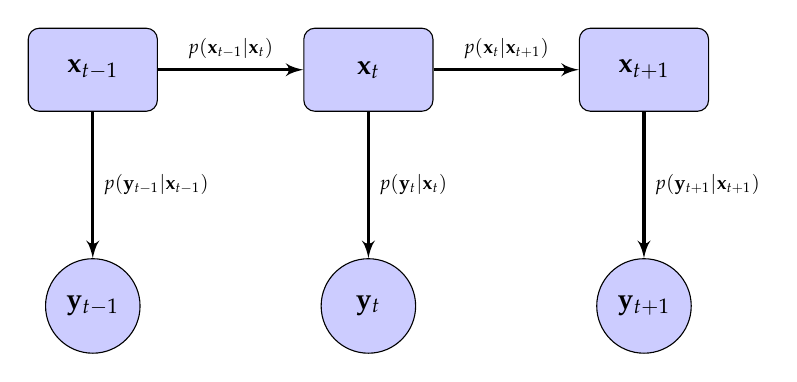
\begin{tikzpicture}[node distance=3.5cm, auto]
        \tikzset{decision/.style={diamond, draw, fill=blue!20, text badly centered,  node distance=2.5cm, inner sep=0pt,align=center}}
        \tikzstyle{block} = [rectangle, draw, fill=blue!20, 
        text width=4em, text centered, rounded corners, minimum height=3em]
        \tikzset{line/.style={draw, very thick, color=black!100, -latex'}}
        \tikzset{circle/.style={shape=circle,draw,minimum size=1.2cm,fill=blue!20,text centered, align=center}}
        \tikzset{decision answer/.style={near start,color=black}}
        
        \node [block] (x1){$\v x_{t-1}$};
        \node [block, right of=x1] (x2) {$\v x_{t}$};
        \node [block, right of=x2] (x3) {$\v x_{t+1}$};
        \node [circle, below of=x1, node distance = 3cm ] (y1){$\v y_{t-1}$};
        \node [circle, below of=x2, node distance = 3cm] (y2) {$\v y_{t}$};
        \node [circle, below of=x3, node distance = 3cm] (y3) {$\v y_{t+1}$};
        
        \path [line] (x1) -- node {\scriptsize $p(\v x_{t-1} | \v x_t)$}(x2);
        \path [line] (x2)-- node {\scriptsize $p(\v x_{t} | \v x_{t+1})$} (x3);
        
        
        \path [line] (x1)-- node {\scriptsize $p(\v y_{t-1} | \v x_{t-1})$} (y1);
        \path [line] (x2)-- node {\scriptsize $p(\v y_t | \v x_t)$} (y2);
        \path [line] (x3)-- node {\scriptsize $p(\v y_{t+1} | \v x_{t+1})$} (y3);
    \end{tikzpicture}
    \caption{Esquematización de un modelo de Markov escondido} \label{dia:hmm}
\end{figure}

\subsection{Predicción, filtrado y suavizado}

Las técnicas de asimilación de datos buscan hacer inferencia estadística en state-space models, es decir que la distribución de interés es $p(\v x | \v y)$. Sin embargo, dado que tenemos muchas realizaciones en el tiempo para $x$ e $y$, debemos ser más específicos. Habitualmente distinguimos 3 distribuciones objetivo de interés:
\begin{itemize}
    \item La distribución predictiva (también llamada de pronóstico o forecast) $p(\v x_t | \v y_{1:s})$ con $s < t$. Esta es la distribución de un estado ``futuro'' usando datos del ``pasado''
    \item La ditribución filtrante (también llamada análisis) $p(\v x_t | \v y_{1:t})$ que informa sobre el estado actual usando observaciones pasadas y actuales
    \item La distribución suavizante $p(\v x_t | \v y_{1:s})$ con $s > t$ que puede ser interpretada como un reanálisis del estado habiendo colectado observaciones futuras al momento sobre el que se hace inferencia.
\end{itemize}

\subsection{Algoritmo \textit{forward-backward}}

En modelos de Markov escondidos, bajo la suposición de que contamos con un modelo de la distribución inicial del estado $p(\v x_0)$, el modelo de transición $p(\v x_t | \v x_{t-1})$ y el modelo observacional $p(\v y_t | \v x_t)$ se puede deducir un algoritmo para obtener de manera secuencial las distribuciones suavizantes. Además, como un subproducto se obtienen las distribuciones filtrantes y las de pronóstico con un grado de separación temporal. 

Si consideramos una ventana de tiempo $t = 1, ..., T$ el algoritmo primero realiza el forward-pass alternando un paso de predicción, en el que obtiene $p(\v x_t | \v y_{1:t-1})$ con un paso de filtrado (también llamado análisis o update) en el que se incorpora la información de la observación a tiempo $t$ y se obtiene $p(\v x_t | \v y_{1:t})$. 

Para $t = 1, ..., T$:
\begin{itemize}
    \item Predicción: $p(\v x_t | \v y_{1:t-1}) = \int p(\v x_t | \v x_{t-1}) p(\v x_{t-1} | \v y_{1:t-1}) d\v x_{t-1}$\label{eq:forward_pred}
    \item Análisis: $p(\v x_t | \v y_{1:t}) \propto p(\v y_t | \v x_t) p(\v x_t | \v y_{1:t-1})$\label{eq:forward_filt}
\end{itemize}
Para hacer la predicción se integra utilizando el modelo de transición. La interpretación de la fórmula es que se calcula la probabilidad de $\v x_t$ dado $\v x_{t-1}$ considerando todos los valores posibles de $\v x_{t-1}$ que obedecen a la distribución filtrante del tiempo anterior. De esta manera, el paso de predicción es el encargado de propagar hacia adelante la distribución del estado. Por otro lado, para hacer el análisis se usa la regla de Bayes y se incorpora $\v y_t$ utilizando el modelo observacional, es decir se actualiza la distribución obtenida en el paso de predicción. Notemos que usamos la convención notacional $\v y_{1:0} = \emptyset$ lo que le da consistencia a las fórmulas ene caso borde de $t = 0$.

Las distribuciones obtenidas en el forward-pass pueden ser utilizadas a su vez para computar las distribuciones suavizantes iterando esta vez hacia atrás, desde el último tiempo hacia el primero de la siguiente manera:

Para $t = T-1, ..., 0$
\begin{itemize}
    \item Suavizado: $p(\v x_t | \v y_{1:T}) = p(\v x_t |\v y_{1:t}) \int \frac{p(\v x_{t+1} | \v x_t)}
    {p(\v x_{t+1} |\v y_{1:t})}
    p(\v x_{t+1} | \v y_{1:T}) d\v x_{t+1}$
\end{itemize}
donde el caso $t = T$ ya está cubierto pues la distribución filtrante para el último tiempo coincide con la suavizante.

La deducción de las fórmulas para predicción, análisis y suavizado están desarrolladas en mayor detalle en el apéndice \ref{appendix:ffbs}.

A pesar de dar una forma general de resolver el problema que plantea la asimilación de datos, en la práctica su aplicación no es tan directa. La integración sobre el espacio de las variables de estado es en general privativa incluso en espacios de dimensionalidad mediana. Por otro lado, hemos hecho la suposición de que contamos con la probabildad de transición $p(\v x_t | \v x_{t-1})$ y esto usualmente no es el caso. El modelo de transición $\mathcal{M}_t$ suele funcionar como una caja negra, de manera que contamos con una forma de muestrear $p(\v x_t | \v x_{t-1})$ pero no necesariamente de evaluar la función de densidad de probabilidad para calcular las integrales necesarias. Existe una gran diversidad de técnicas de asimilación de datos que abordan este problema de distintas maneras. En las secciones subsiguientes describiremos las más relevantes.

\section{Filtro de Kalman}\label{sec:kf}

El filtro de Kalman trabaja sobre una simplificación del problema dado por las escuaciones \ref{eq:transition} y \ref{eq:observation}. Se asume que el modelo de transición de las variables de estado y el modelo observacional son lineales y que las componentes estocásticas se manifiestan como errores gausianos aditivos insesgados. Esto resulta en la siguiente reformulación de las ecuaciones:
\begin{align}
    \v x_t &= \mathbf{M}_t \v x_{t-1} + \gv\eta_t, \label{eq:kf_forward}\\
    \v y_t &= \mathbf{H}_t \v x_t + \gv\nu_t. \label{eq:kf_observational}
\end{align}
donde $\mathbf{M}_t$ y $\mathbf{H}_t$ son operadores lineales y $\gv\eta_t$ y $\gv\nu_t$ son variables aleatorias Gaussianas con media $\v 0$ y matrices de covarianza $\v Q_t$ y $\v R_t$ respectivamente, es decir $\gv\eta_t \sim \mathcal{N}(\v 0, \v Q_t)$ y $\gv\nu_t \sim \mathcal{N}(\v 0, \v R_t)$. Esta configuración del problema asume que tanto el error de modelo como el observacional son insesgados y quedan codificados por completo en las matrices $\v Q_t$ y $\v R_t$.

Si además suponemos que la distribución inicial de $\v x_0$ es Gaussiana, entonces tanto las distribuciones, predictivas y filtrantes serán también Gaussianas. Esto es porque en el paso de predicción, la linealidad del operador de transición preserva la Gaussianidad, lo cual resulta en que en la aplicación de la regla de Bayes en el paso de análisis tengamos verosimilitud y \textit{prior} Gaussianas resultando en una distribución \textit{a posteriori} (la filtrante) también Gaussiana. Este tipo de distribución tiene la propiedad de que puede ser representadas de manera completa a través de dos parámetros: su vector de medias y su matriz de covarianza. Por lo tanto, la tarea del filtro de Kalman es producir secuencias de medias y covarainzas predictivas, $\{\v x_t^f, \v P_t^f\}_{t=1}^{T}$ y medias y covarianzas filtrantes $\{\v x_t^a, \v P_t^a\}_{t=1}^{T}$, de manera que:
\begin{align*}
    p(\v x_t | \v y_{1:t-1}) &\sim \mathcal{N}(\v x_t^f, \v P_t^f) \\
    p(\v x_t | \v y_{1:t}) &\sim \mathcal{N}(\v x_t^a, \v P_t^a)
\end{align*}

Si incorporamos las densidades de probabilidad Gaussianas en las fórmulas de predicción \ref{eq:forward_pred} y análisis \ref{eq:forward_filt} del \textit{forward-pass} se obtienen ecuaciones cerradas para la secuencia de medias y matrices de covarianza de las distribuciones predictivas y filtrantes. Las ecuaciones que se obtienen para el pronóstico son:
\begin{align}
    \v x_t^f &= \mathbf{M}_t \v x_{t-1}^a \label{eq:kf_mean_pred}\\ 
    \v P_t^f &= \v Q_t + \v M_t \v P_{t-1}^a \v M_t^T \label{eq:kf_var_pred}
\end{align}
mientras que para el análisis resulta:
\begin{align}
    \v x_t^a &= \v x_t^f + \mathbf{K}_t (\v y_t - \v H_t \v x_t^f) \label{eq:kf_mean_filter} \\ 
    \v P_t^a &= (\v I - \v K_t \v H_t) \v P_t^f \label{eq:kf_var_filter}
\end{align}
donde $\v K_t = \v P_t^f \v H_t^T(\v R_t + \v H_t \v P_t^f \v H_t^T)^{-1}$ se denomina matriz de ganancia de Kalman, mientras que el término $(\v y_t - \v H_t \v x_t^f)$ son denominadas innovaciones porque dan cuenta de la diferencia entre el pronóstico y las observación. La deducción de estas fórmulas está desarrollada en el apéndice \ref{appendix:kf}

Notemos que la media de los pronósticos es tan solo la propagación hacia adelante de la media filtrante del tiempo anterior. Por otro lado la matriz de ganancia de Kalman funciona como una matriz de pesos que determina si el estado del análisis será más cercano al pronóstico o si le dará más importancia a la observación. 

\paragraph{Ejemplo: oscilador armónico}
Consideramos aquí un sencillo modelo de un oscilador armónico y ejemplificamos cómo usar el filtro de Kalman. Estos sistemas se pueden modelar con la siguiente ecuación diferencial:
\begin{align*}
    \frac{\partial^2 x}{\partial t} &= -\omega^2 x(t)
\end{align*}
donde $\omega$ es la frecuencia angular. Podemos considerar un integrador numérico de Euler semi-implícito para la posición $x$ y la velocidad $v$ en tiempo discretizado a intervalos de longitud $dt$, con lo que obtenemos:
\begin{align*}
    x_t &= (1 - \omega^2 dt^2) x_{t-1} + v_{t-1} dt \\
    v_t &= v_{t-1} - \omega^2 x_{t-1} dt
\end{align*}
que constituye un sistema lineal que permite la expresión:
\begin{align*}
\underbrace{\begin{pmatrix*}
        x_t \\
        v_t
    \end{pmatrix*}}_{\v x_t} = 
\underbrace{\begin{pmatrix*}
        1 - \omega^2 dt^2 & dt \\
        -\omega^2 dt & 1
    \end{pmatrix*}}_{\v M_t} \cdot
\underbrace{\begin{pmatrix*}
        x_{t-1} \\
        v_{t-1}
    \end{pmatrix*}}_{\v x_{t-1}}
\end{align*}
Adicionalmente podemos incorporar al modelo ruido Gaussiano aditivo constante $\gv\eta_t \sim \mathcal{N}(\v 0, \v Q)$ para obtener una expresión como \ref{eq:kf_forward}. Para el modelo observacional consideraremos que sólo obtenemos datos de la posición utilizando la matriz $\v H_t = (0, 1)$ y que estos datos tienen error aditivo $\gv\nu_t \sim \mathcal{N}(\v 0, \v R)$.

Simulamos entonces una trayectoria que consideramos la trayectoria verdadera y de esta obtenemos las observaciones. Utilizando el filtro de Kalman podemos intentar estimar la trayectoria real a través de la asimilación de los datos simulados. En la figura \ref{fig:KF_harmonic_oscillator} podemos ver las trayectorias reales (que no tienen amplitud constante debido al error introducido por $\gv\eta$) y las estimaciones de las medias del filtro. Estas son naturalmente más precisas para la variable observada, sin embargo las correlaciones entre las observaciones y las variables no observadas que utiliza el filtro permiten un seguimiento aproximado de la variable. Es importante señalar que el filtro de Kalman no produce solo una estimación de las medias sino que provee una medida de la incerteza mediante estimaciones de las varianzas. En la figura \ref{fig:KF_bayes} se representan las densidades de probabilidad del pronóstico y del análisis junto con la verosimilitud de la observación para un tiempo fijo que corresponde a la línea de corte vertical del panel superior de la figura \ref{fig:KF_harmonic_oscillator}. El pronóstico actúa como una probabilidad \textit{a priori} que se combina con la verosimilitud, mediante la regla de Bayes que subyace al análisis del filtro de Kalman, para conformar la distribución \textit{a posteriori} que corresponde al análisis. La estimación del análisis mejora al pronóstico utilizando la observación. Además, la incerteza del análisis es menor a la del pronóstico y a la de la observación, lo cual es una propiedad que se hereda de la regla de Bayes.

\begin{figure}[h!]
    \centering
    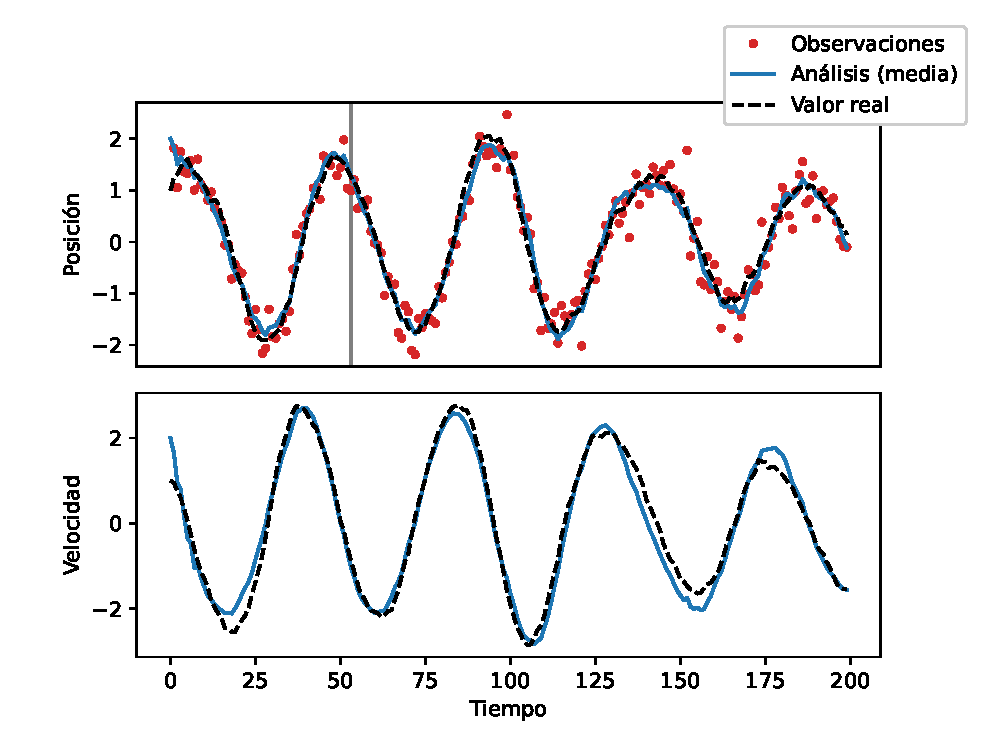
\includegraphics[width=0.75\textwidth]{example_codes/KF_harmonic_oscillator.eps}
    \caption{Trayectorias reales y estimadas mediante el filtro de Kalman. Sólo la posición es observada}
    \label{fig:KF_harmonic_oscillator}
\end{figure}

\begin{figure}[h!]
    \centering
    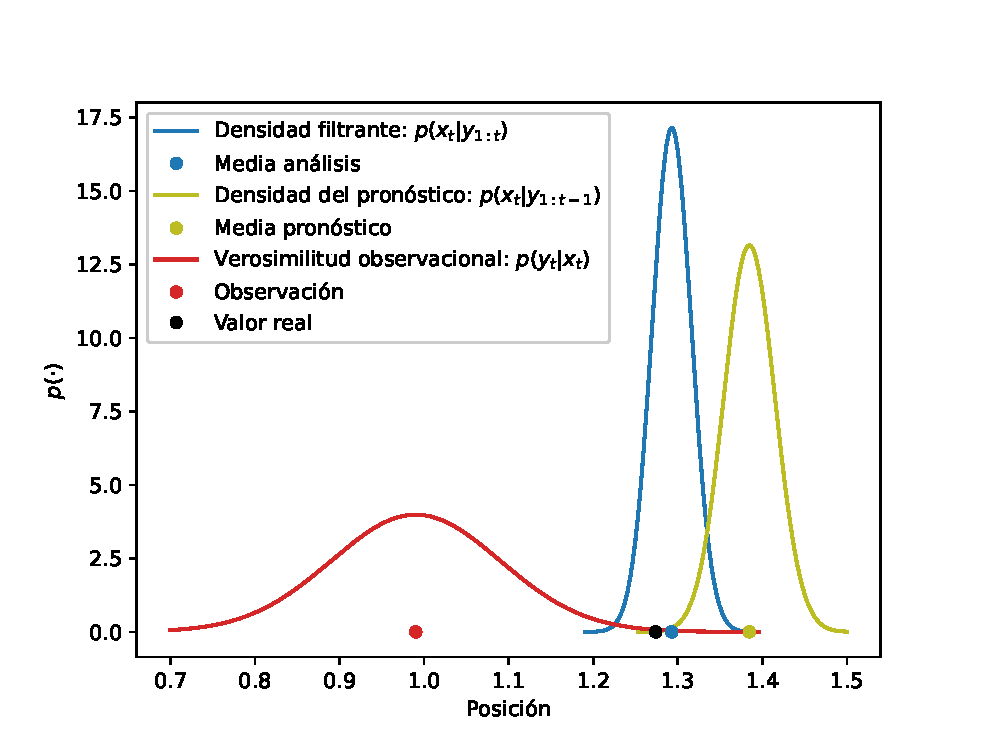
\includegraphics[width=0.75\textwidth]{example_codes/KF_bayes.eps}
    \caption{Funciones de densidad de probabilidad filtrante y de pronóstico junto a la verosimilitud de la observación y el valor real. Corresponde al tiempo indicado por el corte vertical en la figura \ref{fig:KF_harmonic_oscillator}}
    \label{fig:KF_bayes}
\end{figure}

\section{Métodos variacionales}

El problema de obtener un análisis a partir de un pronóstico y una observación puede ser interpretado de manera variacional. Mencionamos brevemente la idea que motiva a los métodos variacionales pues constituyen una familia de técnicas que han sido aplicadas a modelos meteorológicos operacionales y que además dan una perspectiva que enriquece la interpretación de otras estrategias de asimilación de datos. Supongamos que tenemos un pronóstico $\v x^f$ con un error de varianza $\v P^f$ y una observación $\v y$ con un error de varianza $\v R$ y que el operador que mapea el espacio de las variables de estado al espacio de las observaciones se llama $\mathcal{H}$. Si queremos encontrar un valor de análisis $\v x^a$ que minimice el error que introduce el pronóstico y la observación, podemos pensar en minimizar la siguiente función de costo:
\begin{align}
    J(\v x) &= (\v x - \v x^f) {\v P^f}^{-1} (\v x - \v x^f)^T + (\v y - \mathcal{H} (\v x)) \v {R}^{-1} (\v y - \mathcal{H} (\v x))^T \label{eq:3dvar_cost} \\
    &= J^f(\v x) + J^o(\v x)
\end{align}

El primer término da cuenta del costo cuadrático asociado a alejarse del pronóstico y, análogamente, el segundo corresponde a la penalización por alejarse de la observación. Es de esperar entonces que el minimizador de $J$ pondere ambas fuentes de información. De hecho, mientras menor sea el error del pronóstico, mayor será el costo de alejarse de este y para la observación tenemos una situación equivalente. Notemos que esta función de costo supone que los errores sean Gaussianos, aditivos e insesgados. Por otro lado, no hay suposiciones explícitas para el modelo observacional $\mathcal{H}$ y $\mathcal{M}$. De hecho, el modelo de transición ni siquiera está incluído porque se hace la suposición de que ya se cuenta con un pronóstico. Sin embargo, si el pronóstico proviene de un modelo no lineal, no es posible en principio garantizar la Gaussianidad de su error. Sobre el operador observacional también hay que aclarar que dependiendo del método con que se minimice la función de costo, es posible que se necesiten requisitos adicionales: por ejemplo sería esperable que el método de optimización requiera que el operador sea linealizable. En el caso en que este operador sea lineal, $J$ es una función cuadrática con un único mínimo y, de hecho, este coincide con la media del análisis tal como se lo computa en el filtro de Kalman.

La metodología que implementa la minimización de $J$ es comúnmente conocida como 3DVar \citep{Courtier1998}, pero hay que mencionar que el planteo variacional del problema abre la puerta a múltiples variantes, ya que se pueden explorar distintos tipos de optimizadores (por ejemplo simplex, quasi-Newton o gradiente conjugado), distintas condiciones iniciales, precondicionamientos, regularización de $J$, etc. Finalmente mencionamos el método 4DVar \citep{Talagrand1987, Rabier2003} el cual es una extensión de 3DVar pero que procesa una ventana de observaciones simultáneamente, es decir funciona como un suavizador en lugar de como un filtro. El problema que busca optimizar 4DVar es la minimización de una función de costo similar a \ref{eq:3dvar_cost} pero que incluye muchas observaciones. Además se plantea como un problema de optimización con resticciones pues la minimización se hace sujeta a que la solución sea una trayectoria del modelo del que se obtienen los pronósticos.

\section{Técnicas por ensambles}
El filtro de Kalman constituye una técnica robusta que da una solución exacta en el caso de modelos lineales con errores Gaussianos aditivos. En ciertos casos es posible considerar linealizaciónes de los operadores $\mathcal{M}_t$ y $\mathcal{H}_t$ y aplicar el filtro de Kalman tradicional con estas aproximaciones. Este método se denomina filtro de Kalman extendido y también producirá estimaciones de las medias y covarianzas predictivas y filtrantes. Aún así, estas dos técnicas no dan respuesta a dos situaciones frecuentes en las aplicaciones de asimilación de datos. Por un lado, es factible que el modelo no sea linealizabe, ya sea porque es tratado como una caja negra o porque la aproximación lineal es imprecisa. En estas situaciones, los pronósticos serán no Gaussianos y es necesario utilizar técnicas que permitan representar otro tipo de distribuciones. Por otro lado, en modelos meteorológicos es común que el espacio de las observaciones tenga alta dimensionalidad ($\sim 10^5$) y el de las variables de estado aún más ($\sim 10^7$) por lo que computar y almacenar las matrices de covarianza $\v P_t^f$ y $\v P_t^a$ sea prohibitivo \citep{Katzfuss2016}. Para dar cuenta de estos problemas se pueden usar técnicas basadas en partículas o ensambles. Estos, en lugar de representar las distribuciones objetivo a través de sus parámetros como en el filtro de Kalman y el filtro de Kalman extendido, se busca representarlas a través de muestras, es decir un ensamble de puntos en el espacio de las variables de estado. Cada punto muestral suele ser denominado partícula o miembro de ensamble de acuerdo a la técnica en cuestión. Vamos a introducir aquí dos familias de métodos basados en ensambles: los filtros de partículas y los filtros de Kalman por ensambles (EnKFs). Los filtros de partículas permiten, en principio, la representación de distribuciones con formas arbitrarias por lo que pueden ser utilizados en escenarios no Gaussianos. Por otro lado, los EnKFs son habitualmente utilizados para mapear el problema al espacio que generan los miembros del ensamble, el cual tiene una dimensionalidad en general mucho menor que el de las variables de estado haciendo posible el cómputo. Es importante aclarar que ninguna de estas técnicas provee una solución \textit{off-the-shelf} para problemas de asimilación de datos arbitrarios e incluso cada método trae aparejado otro conjunto de dificultades técnicas (por ejemplo la degeneración de pesos en el filtro de partículas o el colapso del ensamble en EnKFs). Tanto para filtros de partículas como EnKFs existe una amplia gama de variaciones e implementaciones que introducen características particulares o que buscan resolver o mitigar algún problema en particular. Comenzaremos introduciendo los filtros de partículas porque estos dan una noción clara de por qué tiene sentido usar muestras para representar distribuciones para luego seguir con los EnKFs.

\subsection{Monte Carlo secuencial}

Los filtros de partículas son también conocidos como métodos de Monte Carlo secuencial ya que utilizan el esquema secuencial de dos pasos de predicción-análisis descrito por las ecuaciones \ref{eq:forward_pred} y \ref{eq:forward_filt}. De hecho, el enfoque de estos métodos es el de resolver las integrales de estas ecuaciones, no de manera explícita sino utlizando las aproximaciones empíricas de las distribuciones implicadas. Si tenemos una función de densidad de probabilidades $p$ y una conjunto de partículas $\{\v x^{(i)}\}_{i=1}^N$ muestreadas de manera independiente con esta probabilidad, i.e. $\v x^{(i)}\sim p$, entonces la aproximación empírica de $p$ basada en esta muestra es:
\begin{align*}
    p(\v x) \approx \frac{1}{N}\sum_{i=1}^N \delta_{\v x^{(i)}}(\v x)
\end{align*}
donde $\delta_{\v a}$ es la delta de Dirac que acumula toda la probabilidad en el punto $\v a$ siendo nula en todo otro punto. Esta aproximación está sustentada en la ley de los grandes números, dado que se pueden aproximar valores esperados en base a la distribución $p$ utilizando la media muestral de las partículas.
\begin{align*}
    \frac{1}{N}\sum_{i=1}^N f(\v x^{(i)}) \xrightarrow{c. s.} \int f(\v x) p(\v x) d \v x
\end{align*}

Existe una generalización de la aproximación de Monte Carlo denominada muestreo de importancia. A pesar de su nombre es un método para aproximar integrales. Cuando no es posible muestrear de $p$ se puede entonces muestrear otra distribución con densidad $q$ que actúe de proxy de $p$. En principio la única condición para $q$ es que su soporte contenga al de $p$. Este método también admite que no se pueda evaluar exactamente $p$ y $q$ sino que sólo podamos evaluar versiones no normalizadas $\tilde{p}$ y $\tilde{q}$ de estas densidades. Entonces, si tenemos un conjunto de partículas $\{\v x^{(i)}\}_{i=1}^N$ tales que $\v x^{(i)}\sim q$, podemos hacer la aproximación dada por las siguientes fórmulas:
\begin{align*}
    \int f(\v x) p(\v x) d \v x &\approx \sum_{i=1}^N w_i f(\v x^{(i)}) \\
    w_i &= \tilde{w}_i / \textstyle\sum_{i=1}^N \tilde{w}_i \\
    \tilde{w}_i &= \tilde{p}(\v x^{(i)}) / \tilde{q}(\v x^{(i)})
\end{align*}
donde $w_i$ son denominados pesos de importancia y $\tilde{w}_i$ son sus versiónes no normalizadas. Por su parte, $q$ es denominada la distribución \textit{propuesta}.

Los métodos de Monte Carlo secuencial producen conjuntos de partículas que aproximan a la distribución filtrante. Estas partícuas además pueden ser ponderadas, es decir pueden traer pesos asociados. Concretamente, para cada tiempo $t$ se obtienen $\{\v x_t^{(i)}, w_t^{(i)}\}_{i=1}^{N}$ tal que sea una aproximación empírica de $p(\v x_t | \v y_{1:t})$.

Los filtros de partículas obtienen estas muestras en dos pasos básicos: primero se muestrean partículas de una distribución propuesta $q$ y luego se computan sus pesos. Con una elección adecuada de $q$ las partículas al tiempo $t$ pueden ser obtenidas a partir de las partículas a tiempo $t-1$ y los pesos pueden ser computados como una actualización de los pesos del tiempo anterior. En particular, dada una muestra pesada $\{\v x_{t-1}^{(i)}, w_{t-1}^{(i)}\}_{i=1}^{N}$ correspondiente al tiempo $t-1$, el procedimiento consiste en:
\begin{itemize}
    \item Muestrear partículas:
        \begin{align*}
            \v x_{t}^{(i)} \sim q(\v x_t | \v x_{t-1}^{(i)}, \v y_t)
        \end{align*}
    \item Actualizar pesos: 
        \begin{align*}
            w_{t}^{(i)} \propto w_{t-1}^{(i)} \frac{p(\v y_t | \v x_t^{(i)}) p(\v x_t^{(i)} | \v x_{t-1}^{(i)})}{q(\v x_t^{(i)} | \v x_{t-1}^{(i)}, \v y_t)}
        \end{align*}
\end{itemize}

Esta implementación es habitualmente llamada SIS (\textit{sequential importance sampling}) y en la práctica tiene el problema de que los pesos suelen concentrarse en una sola partícula, es decir uno de los pesos es prácticamente $1$ mientras que el resto es prácticamente $0$. Este efecto se denomina degeneración del filtro y es indeseable pues la representación muestral de la distribución filtrante pierde expresividad. Además de aumentar el número de partículas existen varias estrategias para mitigar este efecto, la más conocida de ellas es el remuestreo. Este método consiste en muestrar con reemplazo las partículas de la ditribución empirica dada por los pesos. Es decir, una vez computados los pesos se obtiene un nuevo conjunto de partículas con pesos uniformes:
\begin{align*}
    \hat{\v x}_t^{(i)} &\sim \sum_{i=1}^N w_i \delta_{\v x^{(i)}} \\
    \hat{w_i} &= 1 / N
\end{align*}

Esto tiene el efecto que las partículas con mayor peso estarán repetidas y las de menos peso serán eliminadas. A pesar de mitigar la degeneración del filtro causa el problema de empobrecimiento de diversidad del que hablaremos más adelante. No es necesario hacer remuestreo de partículas en cada paso de tiempo y un criterio común para decidir si se hace o no es verificar si el número efectivo de partículas $N_{eff}$ está por debajo de un valor umbral $N_T$. El número efectivo de partículas se puede estimar de la siguiente manera \cite{Arulampalam2002}:
\begin{align*}
    N_{eff} \approx \frac{1}{\sum_{i=1}^N (w_i)^2} \dot{=} \widehat{N_{eff}}
\end{align*}
Este filtro de partículas que incorpora remuestreo suele ser denominado SIR (\textit{sequential importance resampling}) y lo expresamos en forma algortítmica en \ref{algo:sir_pf}.


% TODO: Resolver asignación en algoritmos. Usar := y :~ ?
\begin{algorithm}[H]\label{algo:sir_pf}    
    Muestrear partículas iniciales: $\{\v x_0^{(i)}\}_{i=1}^{N_p} \sim p(\v x_0)$
    
    \For{$t=1, ..., T$}{
        Muestrear partículas de la distribución propuesta: \
        
        \hspace{20pt} $\widehat{\v x}_{t}^{(i)} \sim q(\v x_t | \v x_{t-1}^{(i)}, \v y_t)$ \
        
        Actualizar y normalizar pesos: \
        
        \hspace{20pt} $w_{t}^{(i)} \propto w_{t-1}^{(i)} \frac{p(\v y_t | \widehat{\v x}_t^{(i)}) p(\widehat{\v x}_t^{(i)} | \v x_{t-1}^{(i)})}{q(\widehat{\v x}_t^{(i)} | \v x_{t-1}^{(i)}, \v y_t)}$ \

        Aproximar el número efectivo de partículas: \
        
        \hspace{20pt} $\widehat{N_{eff}} = \frac{1}{\sum_{i=1}^{N_p} (w_i)^2}$ \

        \If{$\widehat{N_{eff}} < N_T$} {
            \begin{flalign*}
                \v x_t^{(i)} &\sim \sum_{i=1}^{N_p} w_i \delta_{\widehat{\v x}_t^{(i)}} & \\
                w_{t}^{(i)} &= 1 / N_p &
            \end{flalign*}            
        }
    }
\caption{Filtro de partículas SIR}
\end{algorithm}

Una de las implementaciones más sencillas de este tipo de filtro es el llamado \textit{bootstrap} y consiste en tomar la distribución propuesta como la probabilidad de transición, i.e., $q(\v x_t | \v x_{t-1}, \v y_t) = p(\v x_t | \v x_{t-1})$. Esto significa que el muestreo de partículas es simpemente aplicar el modelo de transición a todas las partículas del tiempo anterior. Además, las implementaciones más comunes del filtro \textit{bootstrap} hacen remuestreo en cada paso de tiempo. Esto significa que los pesos son sólo calculados para hacer remuestreo pero las partículas que representan a la distribución filtrante tienen pesos uniformes y no hay que almacenarlos. Además esto simplifica el cómputo de los pesos a la expresión $w_{t}^{(i)} \propto p(\v y_t | \v x_t^{(i)})$. En \ref{algo:bootstrap_pf} especificamos este método.

\begin{algorithm}[H]\label{algo:bootstrap_pf}
    Muestrear partículas iniciales: $\{\v x_0^{a, (i)}\}_{i=1}^{N_p} \sim p(\v x_0)$
    
    \For{$t=1, ..., T$}{
        Evolucionar partículas: \
        
        \hspace{20pt} $\v x_{t}^{f, (i)} \sim p(\v x_t | \v x_{t-1}^{a, (i)})$  para $i = 1, ..., N_p$ \
        
        Actualizar y normalizar pesos: \
        
        \hspace{20pt} $w^{(i)} \propto p(\v y_t | \v x_t^{f, (i)})$ \
        
        Remuestrear: \
        
        \hspace{20pt} $\v x_t^{a, (i)} \sim \sum_{i=1}^{N_p} w_i \delta_{\v x^{f, (i)}}$
        }
\caption{Filtro de partículas bootstrap}
\end{algorithm}

La elección de la distribución de transición como distribución propuesta en el filtro de partículas \textit{bootstrap} significa que el muestreo de partículas no es más que evolucionar cada partícula del tiempo anterior utilizando el modelo. Las partículas muestradas constituyen entonces un pronóstico. Esta interpretación no es generalizable al filtro SIR general. Para indicar esto en \ref{algo:bootstrap_pf} usamos el supraíndice $f$ (por \textit{forecast}) en las partículas del pronóstico y $a$ en las de análisis. 

El cómputo de los pesos está dado por la verosimilitud observacional por lo que estos cuantifican cuán afín es cada partícula a la observación. Por su parte, la forma de transformar al conjunto de partículas de pronóstico en una muestra filtrante es a través de el remuestreo. El remuestreo, al ser con reemplazo, tiene el efecto de multiplicar las partículas con pesos altos (cercanas a la observación) y eliminar las partículas con pesos bajos (lejanas a la observación). Este mecanismo se suele comparar con la selección natural, sólo sobreviven y se reproducen las partículas ``más aptas''.

Como se anticipó, el remuestreo introduce otro problema: el empobrecimiento de diversidad. Esto se debe a que tendremos muchas réplicas de las partículas con más peso, es decir una muestra que cubre pbremente el espacio muestral. Este efecto es claramente indeseable y para paliarlo es habitual introducir, luego del remuestreo, un paso en el que las partículas se mutan o se mueven de alguna forma para no tener tantas partículas repetidas. El término mutación proviene de la interpretación del fitro de partículas \textit{bootstrap} como un mecanismo de selección del más apto. Esta modificación de las partículas se puede hacer incorporando pasos de MCMC. También es posible mitigar el problema mediante regularización, utilizando \textit{kernel density estimation} sobre las distribuciones empíricas \citep{Sarkka2013, Arulampalam2002, Ruchi2019}.
% TODO: introducir sin mucho detalle filtros de flujo de langevin y VMPF

% TODO: mejorar este párrafo de ventajas y desventajas de PFs en general
El filtro de partículas SIR tiene la ventaja de hacer pocos requisitos sobre el modelo. En el caso particular del filtro \textit{bootstrap} sólo se necesita evaluar la verosimilitud observacional y muestrear de la probabilidad de transición. Obtener muestra de la probabilidad de transición no es otra cosa que evolucionar el modelo, y este requisito por sí solo significa que el modelo puede ser tratado como una caja negra, una característica deseable en muchas situaciones. Como no hay ninguna suposición sobre las distribuciones, estos métodos pueden ser utilizados en escenarios de no-Gaussianidad y no-linealidad. Por otro lado, este tipo de filtros habitualmente necesitan muchas partículas para tener una buena performance y además padecen de los problemas ya mencionados de degeneración del fitro y empobrecimiento de la diversidad. También es común que muchos pesos sean muy pequeños, lo cual puede causar problemas numéricos. Estos problemas se acentúan en espacios de alta dimensionalidad por lo que en estas situaciones es habitual utilizar filtros de Kalman por ensambles, los cuales introducimos en la siguiente sección.

\subsection{EnKF} \label{sec:enkf}

Los filtros de Kalman por ensambles utilizan muestras para mantener estimaciones de las distribuciones objetivo pero incorporan las fórmulas del filtro de Kalman tradicional para actualizar las partículas (en el contexto del EnKF las partículas suelen ser llamadas miembros del ensamble pero utilizaremos las terminologías de manera intercambiable). Para esto es necesario suponer linealidad sobre el modelo de transición y observacional y también errores aditivos Gaussianos: es decir que trabaja sobre el modelo definido por \ref{eq:kf_forward} y \ref{eq:kf_observational}. En realidad, la suposición de que el modelo de transición es lineal puede ser algo relajada en la práctica pero discutiremos esto más adelante.

Supongamos que a tiempo $t-1$ contamos con un ensamble $\{ \v x_{t-1}^{a, (i)} \}_{i=1}^{N_p}$ que representa al análisis. Por las suposiciones que hemos hecho esta muestra será Gaussiana y al aplicar el modelo transicional sobre cada uno de estos miembros del ensamble podemos obtener un ensamble $\{ \v x_{t}^{f, (i)} \}_{i=1}^{N_p}$ del pronóstico a tiempo $t$ el cual constutuirá una muestra Gaussiana. La pregunta entonces, es cómo obtener a partir de este ensamble otro que represente al análisis. La idea de el EnKF es aplicar la ecuación de actualización de la media del filtro de Kalman tradicional \ref{eq:kf_mean_filter} para cada partícula del pronóstico. Esta es la esencia de los EnKF pero para aplicar el concepto correctamente debemos hacer algunas salvedades.

Para aplicar la actualización del filtro de Kalman ecesitamos computar $\v K_t$ la cual por su parte necesita de la matriz de covarianzas del pronóstico $\v P_t^f$. Sin embargo, a diferencia del filtro de Kalman, aquí no propagamos las matrices de covarianzas en el tiempo, sólo una muestra de la distribución y por ello no disponemos de una representación exacta de esta. De cualquier manera, es natural aproximar $\v P_t^f$ con la matriz de covarianza muestral del ensamble del pronóstico, $\widehat{\v P}_t^f$ para obtener una aproximación $\widehat{\v K}_t$ de la matriz de ganancia de Kalman.

Por otro lado, hay que notar que estamos utilizando sobre cada partícula la fórmula de actualización de la media de la distribución, y cada partícula está siendo actualizada en base a la misma observación. Es posible demostrar que si hacemos esto, la covarianza del ensamble del análisis va a estar subestimada. La solución a este problema consiste en actualizar cada partícula usando una perturbación de la observación original. Para obtener el miembro del ensamble $\v x_t^{a, (i)}$ utilizaremos la observación modificada $\v y_t^{(i)} = \v y_t + \v v_t^{(i)}$ con $\v v_t{(i)} \sim \mathcal{N}(\v 0, \v R_t)$. El origen de este problema y su solución son planteados en \cite{Burgers1998}. El método resultante es denominado EnKF estocástico o EnKF con observaciones perturbadas y en \ref{algo:enkf_pert_obs} está descrito de manera algorítmica. En \ref{appendix:enkf} demostramos que la formulación de este método es correcta.
% TODO: EnKS, mencion? algoritmo?

\begin{algorithm}[H]\label{algo:enkf_pert_obs}
    Muestrear ensamble inicial: $\{\v x_0^{a, (i)} \}_{i=1}^{N_p} \sim p(\v x_0)$
    
    \For{$t=1, ..., T$}{
        \For{$i=1, ..., N_p$} {
            $\gv\eta^{(i)} \sim \mathcal{N}(\v 0, \v Q_t)$ \

            $\v x_t^{f, (i)} = \mathcal{M}_t (\v x_{t-1}^{a, (i)}) + \gv\eta^{(i)}$ \
        }

        % Computar $\widehat{\v P}_t^f$, la covarianza muestral de $\{ \v x_t^{f, (i)} \}_{i=1}^{N_p}$ \

        $\widehat{\v x}_t^f = \frac{1}{N_p}\sum_{i=1}^{N_p} \v x_t^{f, (i)}$ \

        $\widehat{\v P}_t^f = \frac{1}{N_p-1}\sum_{i=1}^{N_p} (\v x_t^{f, (i)} - \widehat{\v x}_t^{f}) (\v x_t^{f, (i)} - \widehat{\v x}_t^{f})^T$ \

        $\widehat{\v K}_t = \widehat{\v P}_t^f \v H_t^T(\v R_t + \v H_t \widehat{\v P}_t^f \v H_t^T)^{-1}$ \

        \For{$i=1, ..., N_p$} {
            $ \v v^{(i)} \sim \mathcal{N}(\v 0, \v R_t)$ \

            $ \v y_t^{(i)} = \v y_t + \v v^{(i)} $ \

            $\v x_t^{a, (i)} = \v x_t^{f, (i)} + \widehat{\v K}_t (\v y_t^{(i)} - \v H_t \v x_t^{f, (i)})$ \
        }

    }
\caption{EnKF estocástico}
\end{algorithm}

Notemos que la suposición de que el modelo de transición es lineal es la suposición que permite asumir que evolucionar los miembros del ensamble hacia adelante va a conservar la Gaussianidad de la muestra. Sin embargo, a diferencia del filtro de Kalman tradicional, no precisamos una expresión matricial $\v M_t$ del operador. El modelo se usa solamente para propagar las partículas hacia adelante por lo cual podemos relajar la hipótesis de linealidad y pensar en un operador general $\mathcal{M}_t$ que si es levemente no lineal podrá preservar la Gaussianidad en los pronósticos y que además puede ser tratado como una caja negra. De hecho, el EnKF es habitualmente presentado como un método apto para modelos no lineales.

% TODO: mejorar este párrafo?
El EnKF que presentamos es solamente una implementación sencilla de esta idea pero la realidad es que existe una gran familia de filtros de Kalman por ensambles desarrollados para diferentes tipos de problemas. Los filtros de raíz cuadrada (EnSRF) y los filtros de Kalman por ensambles ajustados (EAKF) sortean necesidad de perturbar las observaciones, lo cual puede causar subestimación de covarianzas \citep{Whitaker2002, Anderson2001}. Los filtros transformados (ETKF) operan sobre el espacio generado por lso miembros del ensamble y consiguen una mejor eficiencia \citep{Bishop2001}.

En general, los EnKFs son métodos robustos, relativamente fáciles de comprender e implementar y que han sido utilizados en una amplia variedad de problemas. Debido a su popularidad, existen muchas modificaciones para mitigar los problemas más comunes que suele presentar. Los EnKF son especialmente aptos para problemas de gran dimensionalidad ya que pueden representar distribuciones en este tipo de espacios con una cantidad relativamente chica de miembros de ensamble. Además, se pueden optimizar numéricamente y tienen potencial para ser implementados de manera paralela. A pesar de que pueden fallar en modelos altamente no lineales que resulten en pronósticos no Gaussianos, en general pueden dar buena performance incluso en presencia de no linealidades. Esta familia de filtros ha disputado con la técnica variacional 4DVAR como método de asimilación de datos operacional en predicción meteorológica numérica.

\paragraph{Inflación y localización} \

Los EnKFs son utilizados en escenarios de alta dimensionalidad en los que surgen una variedad de problemas. Por un lado, debido a que la cantidad de miembros de ensamble resulta pequeña en comparación con la dimensión de las variables de estado, el error de muestreo asociado puede resultar en que la matriz de covarianza predictiva $\widehat{\v P}_t^f$ esté subestimada o que tenga deficiencias de rango \citep{Miyoshi2011}. Esta situación puede estar incluso profundizada por una mala especificación del error de modelo. Esto puede provocar que la dispersión del ensamble sea muy compacta (esto se suele llamar colapso del ensambles) lo cual da como resultado que la certidumbre sobre la predicción sea mayor de lo que debería ser y por lo tanto la información observacional sea menos considerada por el sistema de asimilación de datos. Como resultado, es posible que el filtro comienze a ignorar las observaciones y diverja de la trayectoria que debería estimar. Un paliativo a esta situación es la llamada inflación de covarianza que consiste en agrandar artificialmente la covarianza predictiva \citep{Anderson1999}. Existen diversas implementaciones de esta idea pero distinguimos la inflación aditiva que consiste en añadir ruido a los miembros del ensamble y la inflación multiplicativa que en general es implementada multiplicando la matriz de covarianzas (o las desviaciones de los miembros del ensamble respecto a su media) por un escalar mayor a $1$. Para mejorar la calidad de la matriz de covarianzas predictiva, además se suele usar localización. Esta metodología consiste en reducir el valor de los términos fuera de la diagonal que correspondan a covarianzas de variables lejanas espacialmente y que por lo tanto no deberían estar muy correlacionadas. Esto se hace porque un número bajo de miembros de ensamble puede provocar correlaciones espúreas que deterioren la calidad de la matriz de covarianzas \citep{Hamill2001}. Utilizando localización se puede mitigar la deficiencia de rango y el error de muestreo. 

\subsection{VMPF}


\chapter{Tratamiento de errores}

\section{Error observacional y de modelo}

Más allá de los desafíos y dificultades de implementación de las técnicas de asimilación de datos discutidas en el capítulo anterior, la performance de estas depende crucialmente de la especificación de el error de modelo y el observacional. Tanto la evolución de las variables de estado en el tiempo como el proceso observacional tienen fuentes de incerteza. De hecho, las metodologías de asimilación de datos hacen uso de nuestro conocimiento sobre estas incertidumbres para ponderar entre la información que brinda el pronóstico producido por el modelo y la observación. Veremos que una representación incorrecta de estos errores, y en particular de la razón entre estos, puede dar lugar a un exceso de confianza en los pronósticos o en las observaciones. Esto puede ocasionar que se degrade la calidad de las estimaciones de las distribuciones filtrantes y potencialmente que el filtro se desicronice de las trayectorias subyacentes sobre las que se intenta inferir.

Las variables de estado evolucionan en el tiempo mediante la aplicación del modelo $\mathcal{M}_t$ de la ecuación \ref{eq:transition} el cual se diseña para representar la dinámica del proceso subyacente. Por supuesto, estos modelos constituyen una representación imperfecta de la realidad que buscan describir. En lo que llamamos error de modelo, no sólo incluímos este error de representatividad sino también los provenientes de aproximaciones para simplificar el cómputo, errores numéricos y posiblemente la incerteza proveniente del desconocimiento de valores exactos de la parametrización de $\mathcal{M}_t$. Llamaremos laxamente $\v Q$ al error de modelo usando la notación en \ref{eq:kf_forward} que corresponde al caso común en que lo consideremos aditivo Gaussiano e insesgado. Por otro lado, el error observacional comprende al error de representatividad del operador $\mathcal{H}_t$, las imperfecciones en su especificación y las incertezas intrínsecas de los instrumentos de medición. Análogamente al error de modelo usaremos $\v R$ para referirnos al error observacional. Tenemos entonces que $\v Q$ y $\v R$ acumulan el error de diversas fuentes de incerteza y que además en ciertos casos, como el conocimiento incompleto sobre los fenómenos que modelamos, no disponemos de una cuantificación de estas incertidumbres.

% TODO: replicar ejemplo pierre

Como hemos visto en \ref{sec:enkf} en métodos basados en ensambles, estos tienen tendencia a colapsar debido a errores de muestreo. El error de modelo cobra una relevancia especial pues está asociada a la dispersión de las partículas del pronóstico y por lo tanto es importante especificarlo correctamente para un buen desempeño del sistema de asimilación. Por su parte, en los filtros de partículas, el error de modelo se relaciona a la incerteza de cada partícula. Muchos filtros de partículas modernos buscan mejorar el muestreo llevando a las partículas a regiones de alta verosimilitud como por ejemplo los filtros de partículas implícitos \citep{Chorin2009, Atkins2013, Zhu2016}, los filtros de flujos de partículas temperados \citep{Daum2009} o el filtro de partículas con mapeo variacional \citep{Pulido2019}. Estos suponen el conocimiento de $\v Q$ y por lo tanto se hace relevante poder acoplarlos con una metodología de estimación de dichos errores.

Se han desarrollado una gran cantidad de métodos para estimar estos errores. En \cite{Stroud2018} se apunta a maximizar la verosimilitud de las innovaciones (la diferencia entre la observación y el pronóstico mapeado al espacio observacional) utilizando inferencia Bayesiana. En otros trabajos se utilizan las covarianzas cruzadas entre innovaciones sucesivas para producir estimaciones de $\v Q$ y $\v R$ (Ver por ejemplo el trabajo seminal de \cite{Mehra1970} y una adaptación moderna basada en esta en \cite{Berry2013}). En el trabajo de \cite{Desroziers2005} se definen estadísticos de diagnóstico basados en las innovaciones que pueden ser utilizados para obtener coeficientes de inflación adaptativos \citep{Li2009}. Notemos que la inflación puede ser vista como un método de estimación del error de modelo puesto que da cuenta de la necesidad de ajustar la incertidumbre de los pronósticos. Otra aproximación al problema, sobre la que nos centraremos aquí, es la maximización de la verosimilitud total a través del algoritmo EM (\textit{expectation-maximization}, \cite{Dempster1977}). Este método fue acoplado con éxito al filtro de Kalman tradicional para estimar $\v Q$ y $\v R$ en \cite{Shumway1982} y con posteridad al filtro de Kalman por ensambles combinado con un suavizador de Kalman por ensambles (ver por ejemplo \cite{Dreano2017}). Un buen compendio de todas estas técnicas se puede encontrar en \cite{Tandeo2020}.

Dentro de toda la variedad de métodos para la estimación de errores observacionales y de modelo distinguimos los métodos \textit{offline} de los \textit{online}. Los primeros toman una ventana de observaciones $\v y_{1:T}$ y dan en base a estas una única estimación para $\v Q$ y $\v R$ para todos los tiempos $t = 1, ..., T$. El algoritmo EM es usualmente implementado de esta manera, utilizando un lote (\textit{batch}) de observaciones (tal es el caso en \cite{Dreano2017, Tandeo2015, Pulido2018}) y aplican el EnKF en combinación con el EnKS. Este procedimiento se adaptó para filtros de partículas en \cite{Lucini2021} sorteando la necesidad de utilizar un suavizador de partículas. En muchas aplicaciones no se utilizan suavizadores porque sólo hay interés en las distribuciones filtrantes y pronósticos y se implementan alternando predicción con análisis. Esto ahorra el costo computacional del suavizado y el almacentamiento de todas las estimaciones anteriores necesarias para el suavizador. En estos escenarios es impráctica o inviable la aplicación de métodos de estimación \textit{offline} y se hace necesario utilizar técnicas \textit{online} (también llamadas secuenciales o adaptativas). Estas producen estimaciones de $\v Q$ y $\v R$ de manera secuencial, es decir en cada ciclo de asimilación y utilizando la información de la observación que está siendo procesada (y no de todo el lote de observaciones de manera simultánea). En el trabajo de \cite{Neal1998} se propone una adaptación \textit{online} para el algoritmo EM y, en el contexto de modelos de Markov escondidos, podemos mencionar el algoritmo propuesto en \cite{Cappe2009} que implementa ideas de EM secuencial acoplados a filtros de partículas y las implementaciones de \cite{Andrieu2003} que utilizan pseudo-verosimilitudes basadas en mini-lotes de datos. También es necesario mencionar que existen implementaciones \textit{online} para estimación de errores que no están basadas en EM como por ejemplo la que se puede encontrar en \cite{Berry2013}.

En el trabajo del cual forma parte esta tesis, desarrollamos un nuevo método \textit{online} de estimación de error de modelo y observacional basado en EM compatible con filtros de partículas y con EnKFs. La técnica combina las ideas del \textit{batch} EM en la versón de \cite{Dreano2017} con las ideas expuestas por \cite{Cappe2009} y \cite{Andrieu2003} y el resultado está publicado en \cite{Cocucci2021}. Para dar una derivación del método desarrollaremos el algoritmo EM tradicional por lotes en \ref{sec:batchEM} y luego haremos la deducción teórica con la que podemos hacer la adaptación secuencial en \ref{sec:onlineEM}. 

\section{Estado aumentado}

En la sección anterior se dicutió la relevancia de utilizar estimaciones apropiadas de los errores involucrados. Los parámetros que codifican a estas incertezas suelen ser llamados parámetros ``estocásticos''. Por otro lado, distinguimos a los parámetros específicos al modelo transicional $\mathcal{M}_t$ los cuales suelen ser llamados parámetros ``determinísticos'' ya que usualmente son cantidades interpretables como parte de la dinámica subyacente de las variables de estado $\v x_t$. Es normal que no se cuente con un parametrización precisa del modelo de transición y por lo tanto se deban tomar recaudos. En parte, y como fue mencionado en la sección anterior, se puede dar cuenta de la imperfección en la parametrización de $\v \mathcal{M}_t$ a través del error de modelo y delegar a la estimación de este las incertezas de los parámetros determinísticos. Sin embargo, con la técnica conocida como ``estado aumentado'', es posible estimarlos individualmente y de esta manera calibrar el modelo. Esta consiste en incorporar los parámetros a las variables de estado e interpretarlas como cantidades no observadas del sistema. Si llamamos $\gv\theta_t$ a los parámetros que queremos estimar, construimos entonces el estado aumentado $\tilde{\v x}_t = (\v x_t, \gv \theta_t)$ (notemos la subindexación $t$ que incluímos porque este método admite que los parámetros varíen en el tiempo). Para poder implementar esta idea es necesario extender $\v H_t$ para que interprete a los parámetros como variables no observadas y a $\v \mathcal{M}_t$ para que actúe sobre estos.

Las técnicas de asimilación de datos pueden inferir sobre variables no observadas ya que la asimilación captura las correlaciones entre estas y las observaciones. En el caso de que esta correlación sea muy débil, el análisis será conservador respecto a la variable no observada que permanecerá cerca del pronóstico. Por lo tanto, este comportamiento se replica para los parámetros en estado aumentado y, en el caso que las correlaciones mencionadas sean los suficientemente fuertes, se podrán obtener estimaciones para los parámetros. Además, como estas estimaciones son secuenciales y siguen la lógica ``pronóstico-análisis'' como el resto de las variables de estado, es posible estimar parámetros con variación temporal dando lugar a un sistema que se auto-calibra \citep{Ruiz2013}. Sin embargo, hay que mencionar que, como los parámetros son utilizados en el modelo para el paso de tiempo subsiguiente, si los cambios en el parámetro son muy bruscos el sistema tardará en capturarlos, de manera que la adaptividad del método está sujeta a que las variaciones temporales de los parámetros sean lo suficientemente lentas como para que el sistema pueda asimilarlas. 

Para la extensión de $\v \mathcal{M}_t$ sobre los parámetros es común considerar que actúa como la identidad sobre los parámetros. Esto significa que si $\gv \theta \in \gv\Theta$ entonces $\v \mathcal{M}_t |_{\gv\Theta} (\gv \theta) = \gv \theta$. Sin embargo también habitual incorporar una caminata aleatoria Gaussiana $\v \mathcal{M}_t |_{\gv\Theta} (\gv \theta) = \gv \theta + \gv\epsilon_t$ con $\gv\epsilon_t \sim \mathcal{N}(\v 0, \gv\Sigma_{\gv\epsilon})$. Esto ayuda a que el pronóstico de los parámetros consiga una mejor exploración del espacio paramétrico. Por supuesto, se puede modelar una dinámica para la evolución de los parámetros si fuera necesario. En el caso que se utilice esta estrategia $\gv\Sigma_{\gv\epsilon}$ cuantifica la magnitud de los pasos de la caminata aleatoria y se constituye como un hiperparámetro que se puede calibrar para mejorar la performance del sistema de asimilación. 

La técnica de estado aumentado suele ser adecuada para muchos parámetros físicos y por lo tanto es tentador utilizarla para el tratamiento de los parámetros estocásticos. Sin embargo, debido a la falta de correlación entre la información observacional y los parámetros estocásticos, el método no produce buenos resultados. En \cite{Delsole2010} se puede encontrar una definición algo más precisa de parámetros determinísticos y estocásticos así como una justificación más completa de por qué aumentar el estado con parámetros estocásticos no puede dar buenas estimaciones.

\section{Algoritmo EM}

El algoritmo EM se utiliza para obtener estimadores de máxima verosimilitud en sistemas parcialmente observados. Es en realidad una metodología general y no una solución \textit{off-the-shelf}. Su aplicación más conocida es en el contexto de aprendizaje no supervisado para hacer \textit{clustering} modelando el problema con una mezcla de Gaussianas \citep{Bishop2006} pero tiene una gran diversidad de utilidades. Comenzaremos dando su forma general, luego su aplicación en lotes para estimación de matrices de covarianzas en \textit{state space models} con error aditivo Gaussiano y finalmente su adaptación \textit{online}.

El algoritmo EM en un modelo probabilístico en el que contamos con una variable observada $\v Y$, variables no observadas $\v X$ y un parámetro $\gv\theta$ el cual describe a la probbilidad conjunta $p(\v X,  \v Y; \gv\theta)$. El objetivo es utilizar datos $\v Y$ para estimar el parámetro $\gv\theta$ mediante la maximización de la verosimilitud $p(\v Y; \gv\theta)$ o equivalentemente, de su logaritmo. Si dotamos a las variables no observadas de una distribución \textit{a priori} $q(\v X)$ podemos obtener la expresión:

\begin{align}
    \log p(\v Y; \gv\theta) &=  \log \int p(\v X, \v Y; \gv\theta) d\v X \\
    &=  \underbrace{\int q(\v X) \log \frac{q(\v X)}{p(\v X | \v Y; \gv\theta)} d\v X}_{KL(\int q(\v X) \rVert p(\v X | \v Y; \gv\theta))} + \underbrace{\int q(\v X) \log \frac{p(\v X, \v Y; \gv\theta)}{q(\v X)} d\v X}_{\mathcal{L}(q, \gv\theta)} \label{eq:elbo_KL}
\end{align}
donde $KL$ es la divergencia de Kullback-Leibler y $\mathcal{L}$ es llamada ELBO (\textit{evidence lower bound}). Es común interpretar a $KL$ como una ``distancia'' entre probabilidades y de hecho, cumple que $KL(q \rVert p) \geq 0$ y se anula sí y sólo si $p = q$ en casi todo punto. Al ser $KL$ mayor o igual a 0, esto significa que $\log p(\v Y; \gv\theta) \geq \mathcal{L}(q, \gv\theta)$, es decir que la ELBO es una cota inferior de la log-verosimilitud.  

El algoritmo EM provee estimaciones $\gv\theta_0, \gv\theta_1, ...$ tales que $\log p(\v Y; \gv\theta_{t+1}) \geq \log p(\v Y; \gv\theta_t)$ que convergen a un máximo local de la verosimilitud \citep{Wu1983}. Como dado un $q$ fijo, la $\mathcal{L}(q,\gv\theta)$ es una cota inferior de $\log p(\v Y; \gv\theta)$ para todo $\gv\theta$, entonces la idea es maximizar $\mathcal{L}(q,\gv\theta)$ primero respecto a $q$ y luego respecto a $\gv\theta$. Supongamos que ya contamos con la estimación de la $t$-ésima iteración, $\gv\theta_t$. Si queremos obtener $q = \argmax\limits_{q}\mathcal{L}(q,\gv\theta_t)$, notemos que la igualdad \ref{eq:elbo_KL} se satisface para todo $q$ por lo que debemos elegir el valor que anule a la divergencia de Kullback-Leibler, es decir $q = p(\v X | \v Y; \gv\theta_t)$. Luego, dejamos fijo $q$ y elegimos $\theta_{t+1} = \argmax\limits_{\gv\theta} \mathcal{L}(q,\gv\theta)$. De esta manera obtendremos que 
\begin{align*}
    \log p(\v Y; \gv\theta_t) &= \mathcal{L}(p(\v X | \v Y; \gv\theta_t), \gv\theta_t) + \overbrace{KL(p(\v X | \v Y; \gv\theta_t) \rVert p(\v X | \v Y; \gv\theta_t))}^{0} \\
    &= \mathcal{L}(p(\v X | \v Y; \gv\theta_t), \gv\theta_t) \\
    &\leq \mathcal{L}(p(\v X | \v Y; \gv\theta_t), \gv\theta_{t+1}) \\
    % &\leq \mathcal{L}(p(\v X | \v Y; \gv\theta_t), \gv\theta_{t+1}) + \overbrace{KL(p(\v X | \v Y; \gv\theta_t) \rVert p(\v X | \v Y; \gv\theta_{t+1}))}^{\geq 0} \\
    &\leq \log p(\v Y; \gv\theta_{t+1})
\end{align*}
y por lo tanto que las estimaciones producidas incrementan la verosimilitud.

Notemos además que una vez elegido $q$ tal que anule a la divergencia de Kullback-Liebler en la iteración $t$ obtenemos que:
\begin{align*}
    \mathcal{L}(p(\v X | \v Y; \gv\theta_t), \gv\theta) &= \int p(\v X | \v Y; \gv\theta_t) \log \frac{p(\v X, \v Y; \gv\theta)}{p(\v X | \v Y; \gv\theta_t)} d\v X \\
    &= \int p(\v X | \v Y; \gv\theta_t) \log p(\v X, \v Y; \gv\theta) d\v X - \int p(\v X | \v Y; \gv\theta_t) \log p(\v X | \v Y; \gv\theta_t) d\v X \\
    &\propto_{\theta} \int p(\v X | \v Y; \gv\theta_t) \log p(\v X, \v Y; \gv\theta) d\v X \\
    &\dot{=} E_{\gv\theta_t}[\log p(\v X, \v Y; \gv\theta)| \v Y]
\end{align*}
es decir que la ELBO se puede expresar como una esperanza condicional una vez que elegimos $q$ que maximiza a $\mathcal{L}$. Debido a esto, la maximización sobre $q$ recibe el nombre de \textit{E-step}. Por otra parte el \textit{M-step} corresponde a la maximización sobre $\gv\theta$. El procedimiento admite entonces la caracterización que presentada en \ref{algo:general_EM} en el que suponemos que se realizan una cantidad prefijada $N_{it}$ de itereaciones, aunque también es posible usar otros criterios de parada.

\begin{algorithm}[H]\label{algo:general_EM}

    Elegir valor inicial $\gv\theta_0$:\

    \For{$t=0, 1, ..., N_{it} $}{
        E-step: \
            Computar $\mathcal{Q}(\gv\theta, \gv\theta_t) = E_{\gv\theta_t}[\log p(\v X, \v Y; \gv\theta)| \v Y]$

        M-step: \
            $\gv\theta_{t+1} = \argmax\limits_{\gv \theta} \mathcal{Q}(\gv\theta, \gv\theta_t)$
    }
\caption{EM general}
\end{algorithm}

La metodología que presentamos tiene la conveniencia de incrementar (o mantener) la verosimilitud en cada paso, sin embargo no garantiza que el máximo encontrado sea un máximo global de la verosimilitud. Por otro lado, cuando la probabilidad conjunta de las variables observadas y no observadas pertenece a la familia exponencial, tenemos simplificaciones importantes en el cómputo; esto no siempre es el caso y existen variantes del algoritmo EM que consideran hacer una maximización parcial el el \textit{M-step} (EM generalizado). Otra generalización consiste en una optimización parcial en la elección de $q$ en el \textit{E-step} (EM incremental, \cite{Neal1998}) que se implementa mediante la incorporación secuencial de las observaciones. Este método ayuda a una convergencia más rápida del algoritmo, que de otro modo tiene una convergencia en muchos casos lenta. Además, es el punto de partida para las versiones \textit{online} del EM que veremos más adelate.

\subsection{Batch EM} \label{sec:batchEM}

Los modelos de Markov escondidos son efectivamente sistemas parcialmente observados que en principio, admiten la aplicación del algoritmo EM. Pero además la estrctura Markoviana de dependencia temporal de las variables no observadas junto a la independencia condicional de las observaciones puede ser utilizada para obtener una expresión más sencilla de la ELBO. Haremos ahora la suposición de que contamos con un modelo de Markov escondido en un intervalo de tiempos $t = 0, 1, ..., T$ para los cuales tenemos variables latentes $\v x_{0:T}$ y observaciones $\v y_{1:T}$. Las propiedades mencionadas sobre modelos de Markov escondidos nos permiten factorizar a la probabilidad conjunta (necesaria para computar la ELBO) como:
\begin{align}
    p(\v x_{0:T}, \v y_{1:T} ; \gv\theta) &= p(\v x_0 ; \gv\theta) \prod_{t=1}^T p(\v x_t | \v x_{t-1} ; \gv\theta) p(\v y_t | \v x_t ; \gv\theta) \\
    &= p(\v x_0 ; \gv\theta) \prod_{t=1}^T p(\v x_t, \v y_t | \v x_{t-1} ; \gv\theta)
\end{align}

Con esta expresión se puede obtener entonces la siguiente para la ELBO correspondiente a la $i$-ésima iteración del método, una vez se eligió a $q$ como la distribución de las variables latentes condicionadas a las observaciones:
\begin{align}
    \mathcal{L}(p(\v x_{0:T} | \v y_{1:T} ; \gv\theta_i), \gv\theta) &\propto_{\gv\theta} \sum_{t=1}^T \int p(\v x_{1:T} | \v y_{1:T} ; \gv\theta_i) \log p(\v x_t, \v y_t | \v x_{t-1} ; \gv\theta) d\v x_{1:T} \\
    &= \sum_{t=1}^T E_{\gv\theta_i} [\log p(\v x_t, \v y_t | \v x_{t-1} ; \gv\theta) | \v y_{1:T}]
\end{align}
En esta expresión hemos quitado el término correspondiente a $p(\v x_0 ; \gv\theta)$ bajo la suposición de que no hay parametros desconocidos en la distribución inicial. Esta suposición no es necesaria y de hecho en \cite{Dreano2017} se estima su media y varianza. Ahora haremos una suposición extra que nos permitirá obtener una forma analítica del gradiente de la ELBO: supondremos que $p(\v x_t, \v y_t | \v x_{t-1} ; \gv\theta)$ pertenece a la familia exponencial. Este supuesto no es extremadamente restrictivo puesto que muchas distribuciones relevantes son de la familia exponencial incluyendo, importantemente, a la Gaussiana. Tendremos entonces que:
\begin{align*}
    p(\v x_t, \v y_t | \v x_{t-1} ; \gv\theta) = h(\v x_t, \v y_t) \exp(\psi(\gv\theta)\cdot s(\v x_{t-1}, \v x_t, \v y_t) - A(\gv\theta))
\end{align*}
donde $s(\v x_{t-1}, \v x_t, \v y_t)$ es llamado el estadístico suficiente, $\psi(\gv\theta)$ la parametrización natural y $h$ y $A$ son funciones \citep{Wasserman2004}. El gradiente de la ELBO respecto al parámetro se puede computar como:
\begin{align}
    \nabla_{\gv\theta} \mathcal{L}(p(\v x_{0:T} | \v y_{1:T} ; \gv\theta_i), \gv\theta) = \nabla_{\gv\theta} \psi(\gv\theta) \cdot \sum_{t=1}^T E_{\gv\theta_i} [s(\v x_{t-1}, \v x_t, \v y_t) | \v y_{1:T}] - T\nabla_{\gv\theta}A(\gv\theta)
\end{align}
con lo cual anulando el gradiente obtenemos la siguiente ecuación
\begin{align} \label{eq:null_elbo_grad}
    \nabla_{\gv\theta} \psi(\gv\theta) \cdot S_i - \nabla_{\gv\theta}A(\gv\theta) = 0
\end{align}
donde usamos la nomenclatura
\begin{align} \label{eq:S_def}
    S_i = \frac{1}{T}\sum_{t=1}^T E_{\gv\theta_i} [s(\v x_{t-1}, \v x_t, \v y_t) | \v y_{1:T}]
\end{align}
El valor del parámetro que cumpla con \ref{eq:null_elbo_grad} será el que maximice la ELBO y por lo tanto el valor subsiguiente del EM, $\gv\theta_{i+1}$. Más precisamente, el valor que anula el gradiente es un punto crítico pero en este caso está garantizado que es un máximo debido a propiedades del Hessiano en familias exponenciales \citep{Wainwright2008}. Notemos que la cantidad $S_i$ un promedio sobre toda la ventana temporal $t=1, .., T$ valores esperados de los estadísticos suficientes condiconados a \textit{todas} las observaciones y computado con la última estimación disponible del parámetro, $\gv\theta_i$. El condicionamiento sobre toda la ventana de observaciones implica que el valor esperado esta siendo computado utilizando las distribuciones suavizantes. El método EM que se obtiene para modelos de Markov escondidos bajo la hipótesis de familia exponencial consiste entonces en un \textit{E-step} en el que computamos $S_i$ (\ref{eq:S_def}) y un \textit{M-step} en el que resolvemos la ecuación que anula el gradiente de la ELBO (\ref{eq:null_elbo_grad}).

\subsubsection*{El caso Gaussiano}
Ahora trataremos el caso en el que el error observacional y de modelo sean aditivos y Gaussianos, es decir que tenemos:
\begin{align}
    p(\v x_t | \v x_{t-1}) &\sim \mathcal{N}(\mathcal{M}_t(\v x_{t-1}), \v Q) \\
    p(\v y_t | \v x_t) &\sim \mathcal{N}(\mathcal{H}_t(\v x_t), \v R)
\end{align}
y buscamos estimar $\gv\theta = (\v Q, \v R)$, las matrices de covarianzas del error de modelo y observacional respectivamente. Notemos que, no estamos considerando que estas matrices cambien en el tiempo, es decir que suponemos que corresponden a toda la ventana temporal. Además, debido a la independencia condicional de las observaciones de los modelos de Markov escondidos, tenemos que $p(\v x_t, \v y_t | \v x_{t-1}) = p(\v x_t | \v x_{t-1}) (\v y_t | \v x_t)$ y como supusimos que $p(\v x_t | \v x_{t-1})$ y $(\v y_t | \v x_t)$ son Gaussianas, esto implica que $p(\v x_t, \v y_t | \v x_{t-1})$ también lo es. Esto implica que seguimos bajo la suposición de familia exponencial que enunciamos anteriormente. La cantidad $S_i$, en este caso puede ser pensada como una tupla $(S_i^{\v Q}, S_i^{\v R})$ y la podemos computar mediante las siguientes expresiones que corresponden al \textit{E-step}:
\begin{align}
    S_i^{\v Q} &= \frac{1}{T}\sum_{t=1}^T E_{\gv\theta_i}[(\v x_t - \mathcal{M}_t(\v x_{t-1}))(\v x_t - \mathcal{M}_t(\v x_{t-1}))^T | \v y_{1:T}] \label{eq:batchEM_SQ} \\
    S_i^{\v R} &= \frac{1}{T}\sum_{t=1}^T E_{\gv\theta_i}[(\v y_t - \mathcal{H}_t(\v x_t))(\v y_t - \mathcal{H}_t(\v x_t))^T | \v y_{1:T}] \label{eq:batchEM_SR}
\end{align}
Por otro lado, la ecuación \ref{eq:null_elbo_grad}, para el caso Gaussiano tiene como solución exactamente a la cantidad $S_i$, con lo cual el \textit{M-step} no requiere ningún cómputo adicional. La verificación de que $\gv\theta = S_i$ anula al gradiente de la ELBO se puede encontar en el apéndice junto con la representación de una densidad Gaussiana multivariada como miembro de la familia exponencial.
% TODO: apendice

Las ecuaciones \ref{eq:batchEM_SQ} y \ref{eq:batchEM_SR}, nos dan fórmulas para computar sucesivas estimaciones de $\v Q$ y $\v R$ y constituyen las fórmulas principales utilizadas en \cite{Dreano2017, Tandeo2015, Pulido2019}. Sin embargo, requieren el cómputo de valores esperados condicionados a la totalidad de la ventana de observaciones, $\v y_{1:T}$. Si se cuenta con una representación de partículas de las distribuciones suavizantes $p(\v x_t | \v x_{1:T})$ para todo $t$, entonces los valores esperados se pueden aproximar con estimadores de Monte Carlo. Notablemente, el EnKS es una técnica que provee estas representaciones y que también es apropiada para sistemas con errores Gaussianos aditivos; por lo tanto es compatible con esta aplicación del EM. En el algoritmo \ref{algo:em_enks} podemos encontrar la implementación de este método.

\begin{algorithm}[H]\label{algo:em_enks}

    Muestrear ensamble inicial: $\{\v x_0^{a, (i)} \}_{i=1}^{N_p} \sim p(\v x_0)$ \

    Elegir valor inicial $\gv\theta_0 = (\v Q_0, \v R_0)$:\

    \For{$i=1, ..., N_{it}$}{
        Computar los ensambles de pronóstico, filtrantes y suavizantes usando EnKF+EnKS con la parametrización $\gv\theta_{i-1}$ \
            
            \begin{align*}
                \{ \v x_t^{f, (j)} \}_{j=1}^{N_p} &\sim p(\v x_t | \v y_{1:t-1}) \hspace{2em} \forall t=1, ..., T \\
                \{ \v x_t^{a, (j)} \}_{j=1}^{N_p} &\sim p(\v x_t | \v y_{1:t}) \hspace{2em} \forall t=1, ..., T
            \end{align*}

        Utilizar los ensambles de pronóstico y filtrantes para computar los suavizantes mediante EnKS \
            \begin{align*}
                \{\v x_t^{s, (j)} \}_{j=1}^{N_p} \sim p(\v x_t | \v y_{1:T}) \hspace{2em} \forall t=1, ..., T
            \end{align*}

        \textit{E-step}: \

            \begin{align*}
                S_i^{\v Q} &= \frac{1}{T} \sum_{t=1}^{T} \frac{1}{N_p} \sum_{j=1}^{N_p} (\v x_t^{s, (j)} - \mathcal{M}_t(\v x_{t-1}^{s, (j)}))(\v x_t^{s, (j)} - \mathcal{M}_t(\v x_{t-1}^{s, (j)}))^T \\
                S_i^{\v R} &= \frac{1}{T} \sum_{t=1}^{T} \frac{1}{N_p} \sum_{j=1}^{N_p} (\v y_t - \mathcal{H}_t(\v x_t^{s, (j)}))(\v y_t - \mathcal{H}_t(\v x_t^{s, (j)}))^T
            \end{align*}

        \textit{M-step}: \
            Asignar nuevos parámetros $\gv\theta_i = (\v Q_i, \v R_i)$ \
            \begin{align*}
                \v Q_i &= S_i^{\v Q} \\
                \v R_i &= S_i^{\v R}
            \end{align*}

    }
\caption{EM-EnKS}
\end{algorithm}

Podemos ver que el algoritmo involucra, para cada iteración, procesar las iteraciones hacia adelante mediante predicción y filtrado con el EnKF, reprocesarlas hacia atrás con el EnKS y luego computar con Monte Carlo las actualizaciones de los parámetros. Las pasadas hacia adelante y hacia atrás provienen de que el EnKF y EnKS son implementaciones del algoritmo \textit{forward-backward}. Esto significa que para utilizar este algoritmo debemos procesar todas las observaciones reiteradas veces. Además del costo computacional, esto implica que las observaciones tienen que ser almacenadas y no se contempla una posible incorporación de nuevas observaciones, situación que sería esperable en un sistema en tiempo real. Aunque el \textit{batch EM} combinado con EnKS es un método robusto para estimar la estrctura general de $\v Q$ y $\v R$ su naturaleza \textit{offline} lo puede hacer impráctico en algunas situaciones y demasiado costoso computacionalmente. Además, no siempre es posible o factible obtener valores esperados respecto a distribuciones suavizantes. Por estos motivos se han desarrollado técnicas \textit{online} o secuenciales de estimación de parámetros estocásticos. 

\subsection{Online EM} \label{sec:onlineEM}

Aquí expondremos el algoritmo \textit{online} basado en EM cuyo desarrollo fue publicado en \cite{Cocucci2021}. El objetivo es obtener una técnica que actualice la estimación del parámetro con cada nueva observación de manera que se puedan descartar las observaciones anteriores que ya han sido procesadas. Si tomamos como punto de partida las ecuaciones \ref{eq:batchEM_SQ} y \ref{eq:batchEM_SR} podemos ver que, cada sumando corresponde a una observación pero que si quisiéramos agregar una observación nueva (correspondiente al tiempo $T+1$) todos estos sumandos deberían ser recomputados. Esto es debido a que los valores esperados están condicionados a toda la ventana observacional anterior, $\v y_{1:T}$. Las nuevas distiribuciones predictivas y filtrantes, $p(\v x_{T+1} | \v y_{1:T})$ y $p(\v x_{T+1} | \v y_{1:T+1})$ pueden ser obtenidas o aproximadas utilizando las anteriores distribuciones predictivas y filtrantes que no necesitan ser cambiadas por la incorporación de la nueva observación. Sin embargo, las distribuciones suavizantes $p(\v x_t | \v y_{1:T})$ deben ser cambiadas por las que tienen en cuenta a la nueva observación, $p(\v x_t | \v x_{1:T+1})$.

En este punto, dado que buscamos procesar observaciones que se hacen disponibles una por una, cambiaremos la notación de las iteraciones del EM y la haremos coincidir con la de las observaciones, puesto que queremos obtener una actualización de los parámetros por cada observación. Entonces consideraremos que tenemos observaciones $\v y_{1:T+1}$ y estimaciones de los parámetros $\gv\theta_0, ..., \gv\theta_T$, y buscaremos, a partir de esto, obtener la estimación $\gv\theta_{T+1}$. Más precisamente, buscaremos actualizaciones de la ELBO, es decir que dada una secuencia $S_1, ..., S_T$ buscaremos actualizar $S_T$ para que incorpore la obeservación $\v y_{T+1}$ de manera de obtener $S_{T+1}$. Esto es porque al hacer una extensión \textit{online} de el \textit{E-step} dotamos de esta propiedad a todo el algoritmo, pues el \textit{M-step} seguirá consistiendo en solucionar \ref{eq:null_elbo_grad} para $\gv\theta$ una vez computado $S_{T+1}$. Comenzamos entonces escribiendo la definición de $S_{T+1}$ como en \ref{eq:S_def} con la nueva notación y desglosando la suma de la siguiente manera:
\begin{align}
    S_{T+1} &= \frac{1}{T+1}\sum_{t=1}^{T+1} E_{\gv\theta_T} [s(\v x_{t-1}, \v x_t, \v y_t) | \v y_{1:T+1}] \\
    &= \frac{1}{T+1}\sum_{t=1}^{T+1} \int p(\v x_{t-1}, \v x_t | \v y_{1:T+1}; \gv\theta_T) s(\v x_{t-1}, \v x_t, \v y_t) d\v x_{t-1:t}\\
    &= \frac{1}{T+1} \left( \sum_{t=1}^{T} \int p(\v x_{t-1}, \v x_t | \v y_{1:T+1}; \gv\theta_T) s(\v x_{t-1}, \v x_t, \v y_t)  d\v x_{t-1:t} \right.\\ 
    &\left. + \int p(\v x_{T}, \v x_{T+1} | \v y_{1:T+1}; \gv\theta_T) s(\v x_{T}, \v x_{T+1}, \v y_{T+1}) d\v x_{T:T+1} \right)
\end{align}
Podemos identificar entonces que los primeros $T$ términos de la suma son simialres a la cantidad $TS_T$ con la salvedad de que en el condicionamiento del valor esperado se incluye la información de la última observación. Haciendo entonces la suposición de que esta última observación no afecta significativiamente a los estados anteriores y sólo influye en el último término se motiva la siguiente aproximación:
\begin{align}
    \widehat{S_{T+1}} &= \left(1 - \frac{1}{T+1}\right) \widehat{S_T} + \frac{1}{T+1} \int p(\v x_{T}, \v x_{T+1} | \v y_{1:T+1}; \gv\theta_T) s(\v x_{T}, \v x_{T+1}, \v y_{T+1}) d\v x_{T:T+1} \\
    &= (1 - \gamma_{T+1}) \widehat{S_T} + \gamma_{T+1} E_{\gv\theta_T} [s(\v x_T, \v x_{T+1}, \v y_{T+1}) | \v y_{1:T+1}] \label{eq:onlineEM_S_rescursion}
\end{align}

Tenemos entonces una recursión que nos permite computar las aproximaciones $\widehat{S_t}$ para todo $t$ de manera recursiva en base a $S_{t-1}$, siempre y cuando contemos con una aproximación inicial $S_0$. Además introducimos $\gamma_t$ que, si bien debe valer $1/t$ para satisfacer \ref{eq:onlineEM_S_rescursion}, puede ser interpretada como una tasa de aprendizaje $\gamma_t \in (0, 1)$, tomando como inspiración técnicas de aproximación estocástica \cite{Legland1997}. Este parámetro va a controlar la ``memoria'' de los estimadores, es decir, pondera la importancia de las estimaciones anteriores respecto al nuevo térimino que incluye a la última observación. Como veremos luego este parámetro se puede calibrar para obtener comportamientos distintos del método en cuanto a convergencia. Notemos que con este esquema se puede flexibilizar la hipótesis de que los parámetros no varíán en el tiempo y podemos considerar casos en que los parámetros varíen lentamente en el tiempo. El método resultante tiene algunas similitudes con el propuesto en \cite{Cappe2009} en el que se utilize una función auxiliar, relacionada a una forma recusiva de suavizado, que permite mantener actualizaciones de $S_t$.

Podemos ver que, a pesar de evitar un suavizado hacia atrás hasta la primera observación, el cómputo del valor esperado en \ref{eq:onlineEM_S_rescursion} implica un suavizado de un paso hacia atrás porque el estadístico $s$ depende de $\v x_T$ y el condicionamiento incluye a $\v y_{T+1}$. De acuerdo a como se compute o aproxime este valor esperado tendremos distintas implementaciones del método. En particular daremos dos posibles formas de aproximar este valor con Monte Carlo. El primero de los métodos está basado en \textit{importance sampling} y está pensado para ser acoplado a filtros de partículas. La elección de la distribución de importancia evita hacer un paso de suavizado explícito. El segundo se basa en EnKF y agrega un paso hacia atrás de suavizado de manera explícita usando EnKS.

\chapter{Modelos epidemiológicos} \label{chp:epi_models}

\section{Modelos compartimentales}

Para modelar la propagación de enfermedades infecciosas, es muy habitual utilizar modelos compartimentales basados en ecuaciones diferenciales. Estos pueden ser utilizados para predecir y comprender situaciones epidemiológicas, ayudar a la toma de decisiones y simular situaciones hipotéticas así como también se pueden utilizar para estimar parámetros. Su origen se remonta a los años 20 del siglo pasado y suele atribuirse a \cite{Kermack1927}. Estos consisten en modelar la población distinguiendo subpoblaciones de acuerdo a categorías epidemiológicas. Por ejemplo, el emblemático modelo SIR, distingue a las subpoblaciones susceptible ($S$), infectada ($I$) y recuperada ($R$). Este se puede expresar mediante el siguiente sistema de ecuaciones diferenciales,
\begin{align} \label{eq:sir}
    \frac{\partial S}{\partial t} &= -\beta \frac{SI}{N}\\
    \frac{\partial I}{\partial t} &= \beta \frac{SI}{N} - \gamma I \\
    \frac{\partial R}{\partial t} &= \gamma I
\end{align}
Estas ecuaciones suponen una población constante de tamaño $N$: notemos que las ecuaciones suman 0 por lo que la población total se mantiene. La velocidad con que los individuos susceptibles se infectan es proporcional a la cantidad total de susceptibles, $S$ y a la proporción de infectados de la población $\frac{I}{N}$. La constante de proporcionalidad $\beta$ es llamada la tasa de infección y cuantifica la transmisibilidad de la enfermedad. Por su parte, la velocidad con que los infectados se recuperan es proporcional a la cantidad de infectados y la constante de proporcionalidad $\gamma$ es llamada tasa de recuperación. El sistema resulta en una epidemia cuando $\frac{\partial I}{\partial t} > 0$ y esto sucede cuando $\frac{\beta S(0)}{\gamma} > N$. El número reproductivo básico, $R_0$ en un modelo epidemiológico suele definirse como la cantidad de infectados directos que provocaría un infectado en una población totalmente susceptible. En este caso se puede computar de manera explícita como $R_0 = \frac{\beta}{\gamma}$. El umbral en el comportamiento del sistema depende entonces de este valor pues para que se de un pico epidemico se debe dar que $R_0 S(0) > N$.  En general $t = 0$ representa un momento en el que la enfermedad estásurgiendo y por lo tanto $S(0) \approx N$. Debido a esto se suele considerar que la condición para tener una epidemia es cuando $R_0 > 1$. 

El modelo SIR, aunque sencillo, merece mención pues tiene los elementos básicos con los que se puede construir un modelo compartimental. Como vimos, la entrada y salida de cada compartimento se describe con una ecuación diferencial y con esta idea se pueden diseñar distintas estructuras de subpoblaciones para describir las situaciones que se deseen modelar. Es común ver en este tipo de modelos la subpoblación de los decesos $D$ que permite distinguir a la porción de la población que muere a causa de la enfermedad, o la subpoblación de los expuestos $E$ se suele ver en modelos para enfermedades virales en que las personas se infectan e incuban el virus sin ser infecciosas antes de pasar al compartimento $I$. De esta manera tenemos modelos como el SEIRD que considera estas subpoblaciones, o el SIS que no tiene en cuenta una categoría de recuperados sino que considera que los individuos, al curarse de la enfermedad vuelven a ser susceptibles. Otros consideran compartimentos que corresponden a los inmunizados mediante vacunación. Habitualmente se representa con un diagrama de flujo cuales son los compartimientos y qué direcciones toma el cambio de estado epidemiológico de acuerdo a las características de la enfermedad. Por ejemplo, en la Figura \ref{dia:sir} podemos ver esta representación para un modelo SIR.
\begin{figure}[h]
    \centering
    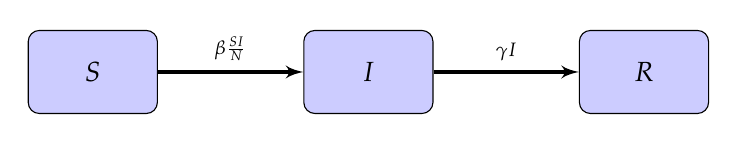
\begin{tikzpicture}[node distance=3.5cm, auto]
        \tikzstyle{block} = [rectangle, draw, fill=blue!20, 
        text width=4em, text centered, rounded corners, minimum height=3em]
        \tikzset{line/.style={draw, very thick, color=black!100, -latex'}}
        
        \node [block] (S){$S$};
        \node [block, right of=S] (I){$I$};
        \node [block, right of=I] (R){$R$};
        
        \path [line] (S) -- node {\scriptsize $\beta \frac{SI}{N}$} (I);
        \path [line] (I) -- node {\scriptsize $\gamma I$} (R);

    \end{tikzpicture}
    \caption{Diagrama para un modelo SIR} \label{dia:sir}
\end{figure}

En, general podemos distinguir 3 tipos distintos de compartimentos: aquellos que actúan de fuente, es decir que solo decrecen o se mantienen, y por lo tanto los términos en las ecuaciones diferenciales son sólo negativos, los compartimentos intermedios, cuyas ecuaciones incluyen términos positivos y negativos y finalmente los compartimentos que actúan de resumidero, es decir que sólo crecen o se mantienen los cuales sólo incluyen términos positivos. Por ejemplo, en el modelo SIR el compartimento $S$ actúa a modo de fuente, $I$ es un compartimento intermedio y $R$ actúa de resumidero. Típicamente las trayectorias de las fuentes tienen una forma sigmoidea decreciente y las de los resumideros son sigmoideas decrecientes mientras que los compartimientos intermedios suelen exhibir un comportamiento con forma de campana. En la figura \ref{fig:sir_example} se puede observar esto en las trayectorias generadas por un modelo SIR.

\begin{figure}[h]
    \centering
    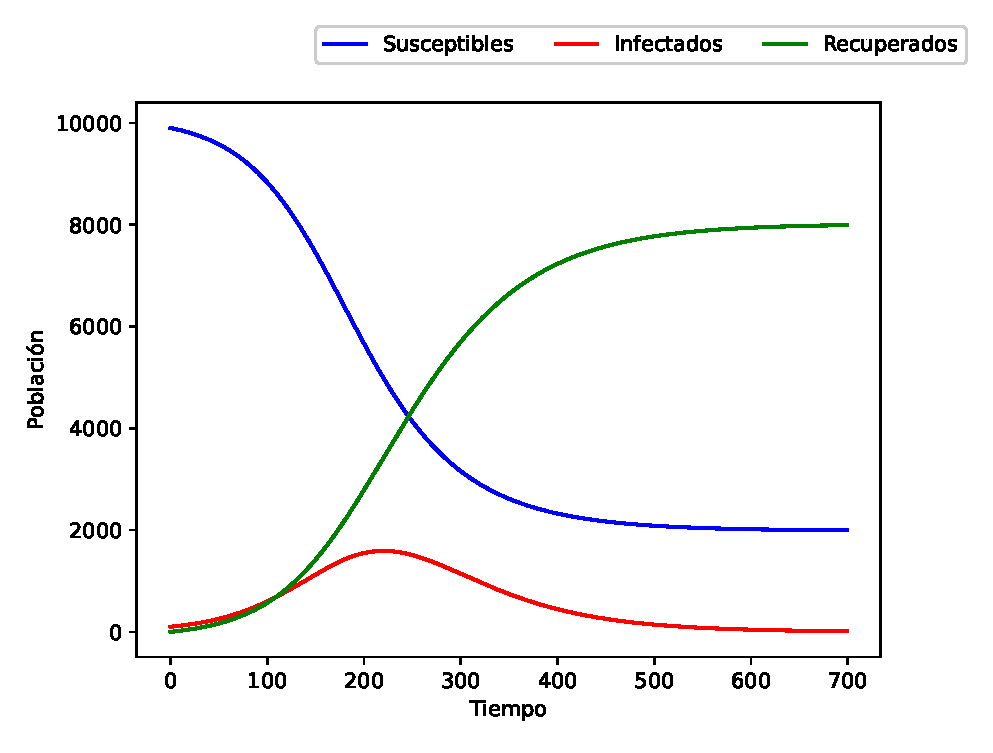
\includegraphics[width=0.75\textwidth]{sir_example.eps}
    \caption{Trayectorias de suceptibles, infectados y recuperados para un modelo SIR básico}
    \label{fig:sir_example}
\end{figure}

La incorporación de compartimentos le da gran adaptabilidad a estos modelos. Sin embargo, se considera que las subpoblaciones representadas en cada uno de estos compartimentos se mezcla de manera homogénea con lo cual no se representan los efectos que provienen de las complejidades del comportamiento de los individuos. Como veremos más adelante, los modelos basados en agentes se focalizan en modelar cada individuo de manera de dar cuenta de las consecuencias de las interacciones en esta micro-escala. Por otro lado, la representación mediante ecuaciones da la posibilidad de analizar formalmente el comportamiento del sistema para, por ejemplo, idententificar puntos de equilibrio, umbrales entre distintos tipos de soluciones o cálcuos explícitos del número reproducivo básico \citep{Murray2007}.

Además de la incorporación de subpoblaciones relacionadas a los estados epidemiológicos, los modelos compartimentales pueden incluir otras características. Por ejemplo, se pueden utilizar variables espaciales acopladas a términos de difusión en las ecuaciones para representar la dispersión territorial de las enfermedades \citep{Noble1974}. También se utiliza estratificación por edades para diferenciar el efecto de la enfermedad en distintos sectores de la población y codificar el contacto entre los distintos rangos etarios \citep{Hethcote2000}. Además se puede modelar la espacialidad a través de la determinación de áreas, por ejemplo barrios en una ciudad, cada una con sus propias subpoblaciones de susceptibles, infectados etc. y describiendo la interacción entre estos lugares \citep{Klepac2018}. Con el advenimiento de la pandemia de COVID-19 se desarrollaron un gran número de modelos compartimentales con características especiales para expresar determinados rasgos propios de esta enfermedad y que se han utilizado para diversos fines tales como la estimación de parámetros epidemiológicos, la evaluación de medidas de control o la predicción de tendencias en los picos de contagios. Por ejemplo, el modelo de \cite{Evensen2020} utiliza estratificación por edades y compartimentos para representar de subpoblaciones bajo distintos tipos de cuarentena y es utilizado para estimar $R_0$ y hacer predicciones en distintos escenearios en diferentes países. El modelo de \cite{Arenas2020} también incluye estratificación por edades pero también incorpora patrones de movimiento en distintas regiones de España, compartimentos para los hospitalizados y otras cararterísticas incluídas para adaptar el esquema al COVID-19. En general, cuando tenemos una segmentación de la población en $K$ grupos (ya sea rango etario, locación o alguna otro) tenemos una réplica del sistema de ecuaciones por cada uno de ellos. La interacción entre estos se representa mediante una matriz $K \times K$. Si extendemos las ecuaciones del modelo SIR a un modelo multi-grupos tendremos las siguientes ecuaciones para $i=1, ..., K$:
\begin{align}
    \frac{\partial S_i}{\partial t} &= -\beta \sum_{j=1}^{K}c_{ij}\frac{S_i I_j}{N}\\
    \frac{\partial I_i}{\partial t} &= \beta \sum_{j=1}^{K}c_{ij}\frac{S_i I_j}{N} - \gamma I_i \\
    \frac{\partial R_i}{\partial t} &= \gamma I_i
\end{align}
donde $c$ es la matriz de conectividad, de manera que la interacción entre el grupo $i$ y y el $j$ está cuantificado por $c_{ij}$.

\section{Inferencia en modelos compartimentales}

Los modelos epidemiológicos por sí solos pueden ser útiles para entender algunos fenómenos respecto a las dinámicas de contagio o los posibles efectos de medidas de control en escenarios hipotéticos. Sin embargo, la parametrización que se utilice puede cambiar drásticamente el comportamiento de los modelos y se hace importante la estimación de parámetros para un mejor ajuste del modelo a los datos o para obtener pronósticos más certeros. Por estos motivos es normal acoplar al modelo alguna técnica de inferencia que permita realizar esta tarea. En particular, la asimilación de datos provee, por un lado técnicas para estimar parámetros como el estado aumentado y por otro mejora los pronósticos de las mismas variables de estado incorporando la información de las observaciones. Además de esto, la asimilación de datos está disñada de manera que es natural el tratamiento de variables no observadas, y en un sistema epidemiológico es normal que haya observaciones incompletas (por ejemplo que sólo se observe la subpoblación de infectados y muertos pero no se observe ninguna de las otras). 

Los trabajos \cite{Ionides2006} y posteriormente \cite{Shaman2012, Shaman2013} constituyen excelentes ejemplos de la aplicación de técnicas modernas de asimilación de datos en modelos epidemiológicos. En \cite{Ionides2006} se utiliza, para un modelo compartimental para el cólera, la técnica de filtros iterados para estimar variables de estado y prámetros estocásticos y físicos. La técnica está basada en el uso de estado aumentado pero con la variante de que se pasa repetidas veces el filtro y en cada iteración se reduce la varianza del parámetro de estado aumentado de tal manera que el valor se va estabilizando en un valor fijo que corresponde al máximo de la verosimilitud. Además se utiliza un filtro de partículas lo cual permite la inferencia en escenarios de no linealidad. Por otro lado, en los trabajos de \cite{Shaman2012, Shaman2013} se aplica el EAKF, una variante del EnKF, a un modelo SIRS para predecir picos de gripe y estimar parámetros relacionados a $R_0$ mediante estado aumentado. Más recientemente, ha habido aplicaciones para modelos de COVID-19. En \cite{Li2020} se utilizan filtros iterados pero con el EAKF para estimar casos no reportados en China. en \cite{Evensen2020} se aplica una técnica basada en suavizadores de Kalman por ensambles llamada ESMDA (\textit{Ensemble Smoother with Multiple Data Assimilation}) para calibrar la parametrización del modelo y, en particular, estimar el número de reproducción efectivo en un modelo compartimental. Por otro lado en \cite{Ghostine2021} se utiliza el EnKF para estudiar el efecto de la vacunación con datos de Arabia Saudita.

A pesar de que las aplicaciones de técnicas de asimilación de datos a modelos epidemiológicos se comienzan a popularizar no se ha hecho particular foco en la estimación de errores observacionales y de modelo. Estas cantidades no sólo tienen interés en sí mismo para la comprensión de las incertezas del sistema sino que, como hemos visto en el Capítulo \ref{chp:error_treatment}, también afectan en la performance del sistema. En particular, el error observacional en modelos epidemiológicos tiene la complejidad de estar relacionado al reporte de casos lo cual puede ser una fuente de información poco precisa y cuya incereteza varía en el tiempo. Por estas cualidades realizamos para esta tesis experimentos preliminares de aplicación de el algoritmo EM online presentado en la sección \ref{sec:onlineEM} cuyos resultados presentamos a continuación.

\subsection{Experimento: observaciones sintéticas} \label{sec:online_em_seird_synthetic}
Para mostrar algunas de las capacidades de el EnKF acoplado con el EM online en un modelo epidemiológico realizamos un experimento con observaciones sintéticas sobre un modelo SEIRD definido por las siguientes ecuaciones diferenciales:
\begin{align} \label{eq:seird}
    \frac{\partial S}{\partial t} &= -\beta \frac{SI}{N}\\
    \frac{\partial E}{\partial t} &= \beta \frac{SI}{N} - \gamma_E E \\
    \frac{\partial I}{\partial t} &= \gamma_E E - \gamma_I I \\
    \frac{\partial R}{\partial t} &= \alpha \gamma_I I \\
    \frac{\partial D}{\partial t} &= (1-\alpha) \gamma_I I
\end{align}
donde $S$, $E$, $I$, $R$ y $D$ representan a los susceptibles, expuestos, infectados, recuperados y muertos respectivamente. $\beta$ es la tasa de infección, $\gamma_E$ determina la velocidad con que los expuestos pasan a ser infectados y $\gamma_I$ la tasa a la que los infectados se recuperan o mueren. La proporción de infectados que mueren es $\alpha$ y la que se recupera $1 - \alpha$. El sistema se puede representar mediante el diagrama de la Figura \ref{dia:seird}. 

\begin{figure}[h]
    \centering
    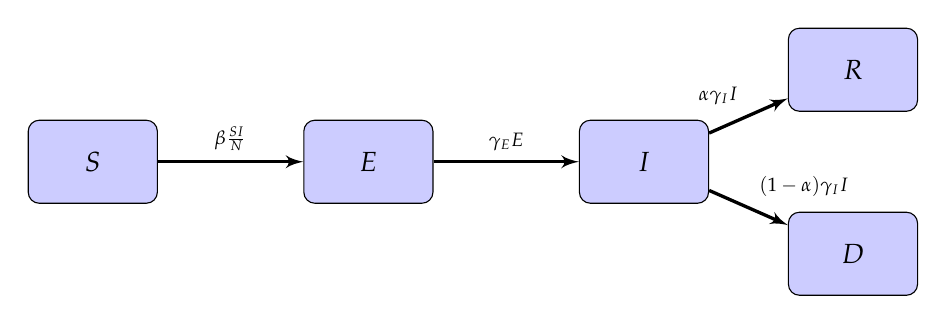
\begin{tikzpicture}[node distance=3.5cm, auto]
        \tikzstyle{block} = [rectangle, draw, fill=blue!20, 
        text width=4em, text centered, rounded corners, minimum height=3em]
        \tikzset{line/.style={draw, very thick, color=black!100, -latex'}}
        
        \node [block] (S){$S$};
        \node [block, right of=S] (E){$E$};
        \node [block, right of=E] (I){$I$};
        \node [block, above right = 0.1cm and 1cm of I] (R){$R$};
        \node [block, below right = 0.1cm and 1cm of I] (D){$D$};
        
        \path [line] (S) --  node {\scriptsize $\beta \frac{SI}{N}$} (E);
        \path [line] (E) --  node {\scriptsize $\gamma_E E$} (I);
        \path [line] (I) --  node {\scriptsize $\alpha \gamma_I I$} (R);
        \path [line] (I) --  node {\scriptsize $(1-\alpha) \gamma_I I$} (D);

    \end{tikzpicture}
    \caption{Diagrama para un modelo SEIRD} \label{dia:seird}
\end{figure}

Consideramos que las observaciones corresponden a los infectados acumulados y a los muertos. Los infectados acumulados, que lamaremos $I_{tot}$ pueden ser computados como la suma de las variables $I$, $R$ y $D$. Por lo tanto el operador observacional se puede escribir en forma matricial como:
\begin{align*}
    \v H = 
    \begin{pmatrix}
        0 & 0 & 1 & 1 & 1 \\
        0 & 0 & 0 & 0 & 1 
    \end{pmatrix}.
\end{align*}
\begin{figure}[h]
    \centering
    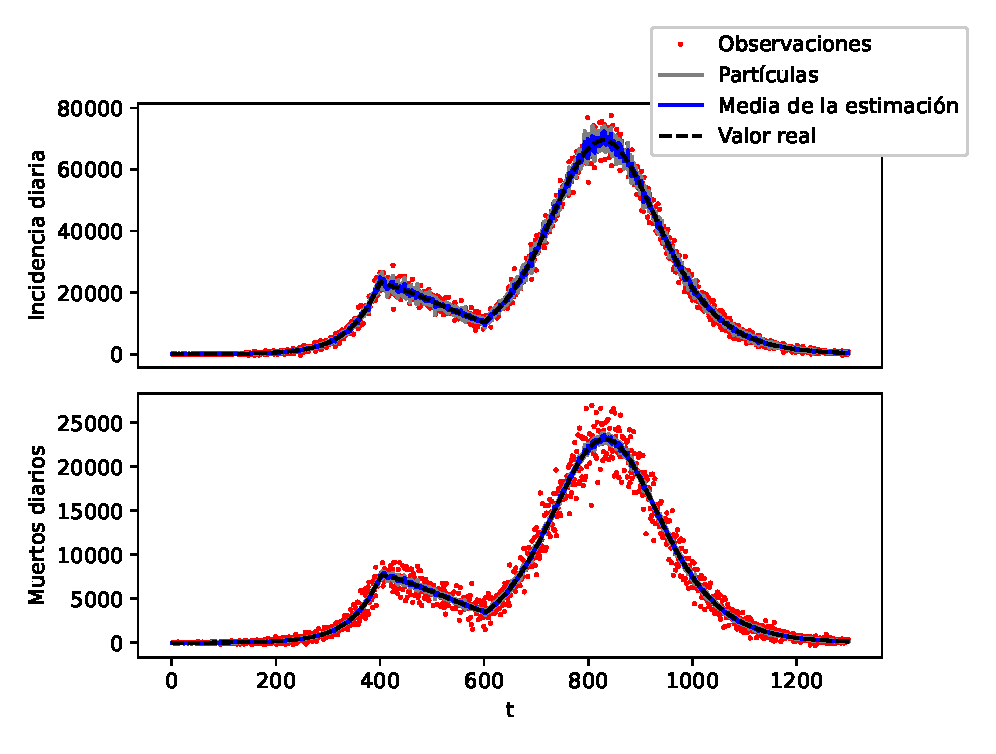
\includegraphics[width=0.75\textwidth]{figs/seird_online_em_aug_state_state_vars.eps}
    \caption{Trayectorias reales, observaciones y estimaciones para los infectados diarios (incidencia diaria) y muertos diarios utilizando el modelo SEIRD}
    \label{fig:seird_online_em_aug_state_state_vars}
\end{figure}
\begin{figure}[h]
    \centering
    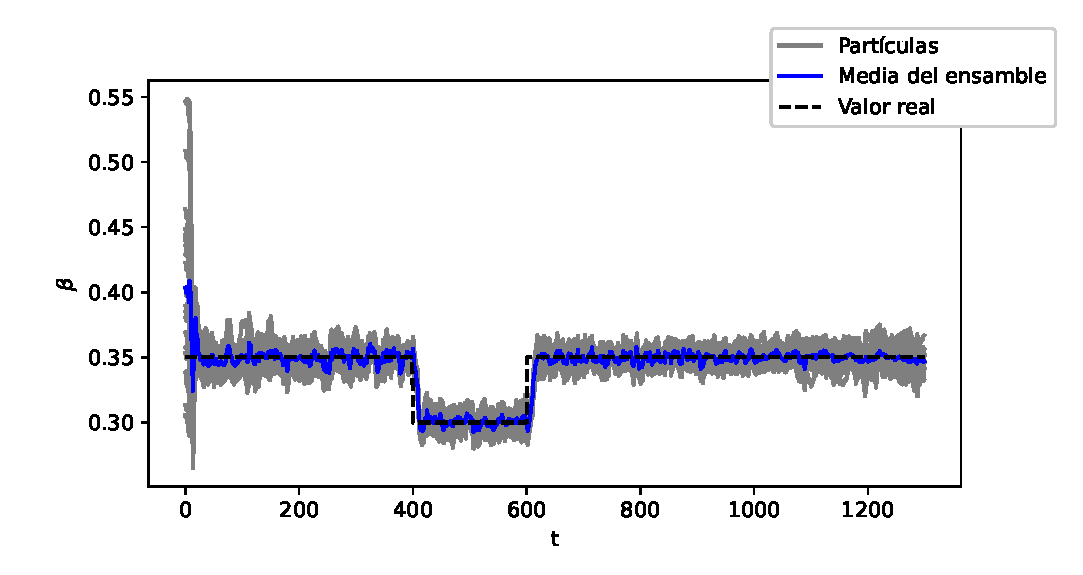
\includegraphics[width=0.75\textwidth]{figs/seird_online_em_aug_state_beta.eps}
    \caption{Valor real y estimaciones de la tasa de infección $\beta$}
    \label{fig:seird_online_em_aug_state_beta}
\end{figure}
\begin{figure}[h]
    \centering
    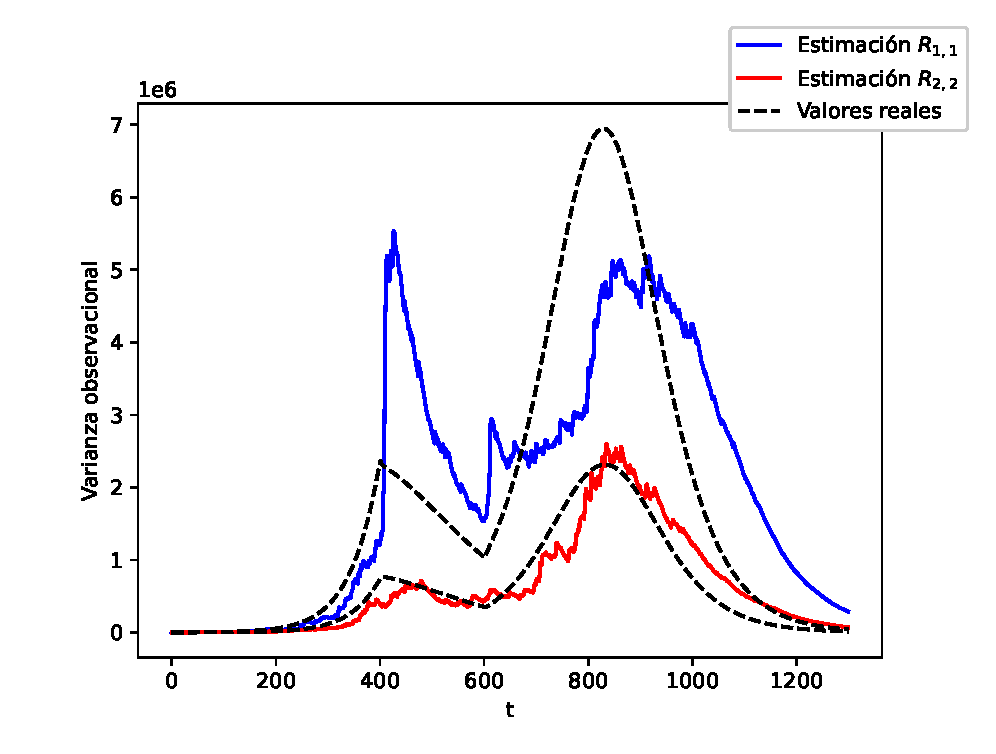
\includegraphics[width=0.75\textwidth]{figs/seird_online_em_aug_state_R.eps}
    \caption{Valores reales y estimados mediante EM online de las varianzas de errores observacionales. Estas corresponden a los dos valores de la diagonal de las matrices de covarianzas $\v R_t$}
    \label{fig:seird_online_em_aug_state_R}
\end{figure}

En la Figura \ref{fig:seird_online_em_aug_state_state_vars} se muestran los valores observados y reales de los infectados y muertos diarios junto con las correspondientes estimaciones. Se ve que el error observacional es proporcional al valor real como se especificó anteriormente y que las estimaciones de las variables sicronizan muy bien con los valores reales. El efecto de variación temporal sobre la tasa de infección $\beta$ explica el efecto de que el sistema produzca dos picos epidémicos. En la Figura \ref{fig:seird_online_em_aug_state_beta} se puede ver que las estimaciones de $\beta$ pueden capturar correctamente el cambio temporal del parámetro. Existe un retardo en las estimaciones para sincronizar luego de los cambios abruptos de la tasa de infección lo cual es habitual para técnicas de estado aumentado debido a que la asimilación tiene cierta inercia hacia valores previos y esto se corrige a medida que las observaciones se van asimilando. Finalmente, en la Figura \ref{fig:seird_online_em_aug_state_R} tenemos las estimaciones de $\v R_t$ producidas por el EM \textit{online} junto a los valores reales utilizados para generar las observaciones. A pesar de haber desvíos sustanciales de las estimaciones respecto a las trayectorias reales es evidente que el algoritmo EM percibe los cambios en $\v R_t$ y da aproximaciones que están en la misma escala. En este experimento utilizamos una tasa de aprendizaje $\alpha = 0.6$ lo que configura al algoritmo para tener ``poca memoria'' dándole más importancia a las observaciones que se están siendo procesadas y no tanto a las estimaciones anteriores. Realizamos réplicas de este mismo experimento con otros valores de $\alpha$ y se obtienen estimaciones menos ruidosas pero que reaccionan más lentamente a los cambios del parámetro.

Al error observacional lo consideraremos Gaussiano y aditivo mientras que a $\v R_t$, la matriz que especifica su varianza a tiempo $t$, la consideraremos diagonal, es decir sin correlación entre los errores. La varianza para el error en la primera variable observada la tomaremos proporcional a los infectados confirmados diarios,  i.e., $(\v R_t)_{1,1} \propto I_{tot}(t) - I_{tot}(t-1)$. Análogamente, para la segunda variable observada tomamos $(\v R_t)_{2,2} \propto D(t) - D(t-1)$. El parámetro $\beta$ será definido como una función constante a trozos. En particular, tendrá un valor de $0.35$ en toda la ventana temporal excepto por el intervalo donde $t \in (400, 600)$ donde su valor será $0.3$. Esto tiene el efecto de que el número de casos aumente, después maine temporalmente para luego volver a crecer. Esta configuración para $\beta$ y $\v R_t$ se utilizará para generar las observaciones sintéticas pero será desconocida para el sistema de asimilación: $\beta$ se estimará mediante estado aumentado mientras que $\v R_t$ a través del EM \textit{online}.

\subsection{Experimento: datos COVID-19 de Argentina}
Como demostración de la potencial viabilidad de la técnica en modelos epidemiológicos realizamos otro experimento similar al de la Sección \ref{sec:online_em_seird_synthetic} pero utilizando los datos de COVID-19 en Argentina provistos por el Ministerio de Salud. El experimento tiene una configuración similar al de observaciones sintéticas que describimos anteriormente pero incorporamos además la tasa de mortalidad que llamaremos $\gamma_D$ y es computable como $(1-\alpha) \gamma_I I$ según las Ecuaciones \ref{eq:seird}.

Cuando se tienen parámetros en el estado aumentado (tal como se expone en la sección \ref{sec:augmented_state}) las caminatas aleatorias que se utilizan para que las estimaciones exploren el espacio paramétrico tienen el efecto de actuar como error de modelo. Por lo tanto, estas intereactúan con el resto del sistema, con las estimaciones de $\v R$, y con el comportamiento de la media y dispersión de las variables de estado (ver Sección \ref{sec:model_obs_error}). En este experimento parametrizamos las caminatas aleatorias con un valor $\sigma^2$ de modo que la amplitud de los pasos es Gaussiana con media 0 y varianza $\sigma^2$ para $\beta$ y $\sigma^2/100$ para $\gamma_D$. Para estudiar su efecto corrimos el experimento para distintos valores de $\sigma^2$. 

En la Figura \ref{fig:seird_vars_arg_data} se grafican los infectados y muertos diarios observados y estimados para el caso de $\sigma^2 = 0.015$. Las trayectorias estimadas están prácticamente superpuestas a las observaciones y la escala impide apreciar la dispersión del ensamble sin embargo este no está colapsado. Los resultados para otros valores de $\sigma^2$ son similares pero la dispersión del ensamble tiende a ser menor cuando se aumenta su valor.

Las estimaciones de $\beta$ y $\gamma_D$ están en la Figura \ref{fig:seird_params_arg_data}. El comportamiento global de los parámetros es similar para todos los valores de $\sigma^2$ pero a medida que este valor aumenta las estimaciones son más ruidosas y con mayor varianza.
La tasa de infección es mayor al comienzo de la pandemia y alrededor de los picos de casos, notablemente en el que corresponde a finales de 2021. Por otro lado la tasa de mortalidad es mayor al comienzo de la ventana temporal y se va reduciendo en el tiempo de manera que el incremento en muertos en la última ola se explicaría según este modelo por el aumento de casos pero no por una mayor letalidad de la enfermedad.

Finalmente, en la Figura \ref{fig:seird_R_arg_data} se pueden ver las estimaciones de las varianzas de los errores observacionales $(\v R_t)_{1,1}$ y $(\v R_t)_{2, 2}$. En este caso es notable como el valor de $\sigma^2$ afecta a las estimaciones que produce el EM \textit{online}: el comportamiento es muy similar para distintos vaalores de $\sigma^2$ pero la escala es muy diferente. Esto se debe a la interacción entre el error de modelo y observacional. Es esperable que mietras mayor sea el error de modelo el sistema le de más importancia a las observaciones. El error que corresponde a la primera variable observada, los infectados acumulados, tiene un pico notable alrededor de la primera ola y otro en la ola de finales de 2021 pero este último se hace menos importante a medida que aumenta $\sigma^2$. Por su parte, el error que corresponde a los fallecidos acumulados es mayor al comienzo de la pandemia y luego se reduce y se estabiliza.

Los resultados dependen de la elección de las caminatas aleatorias en los parámetros dentro del estado aumentado ya que estos tienen el efecto de inyectar error de modelo al sistema. De hecho, podemos ver que al aumentar el valor de $\sigma^2$ se pierde credibilidad en el modelo porque este pasa tener mayor error. Esto resulta en que el sistema de asimilación de datos de mayor importancia a las observaciones y que se reduzca el error observacional estimado por el EM \textit{online}. En la figura \ref{fig:seird_params_arg_data} se aprecia que al aumentar la varianza de las caminatas aleatorias las estimaciones de los parámetros se hacen más ruidosas: esto es un comportamiento típico de sobreajuste las observaciones. El sistema le da demasiada credibilidad a los datos y por lo tanto las trayectorias de las variables de estado (incluídas las del estado aumentado) absorben el error de las observaciones.

\begin{figure}[h]
    \centering
    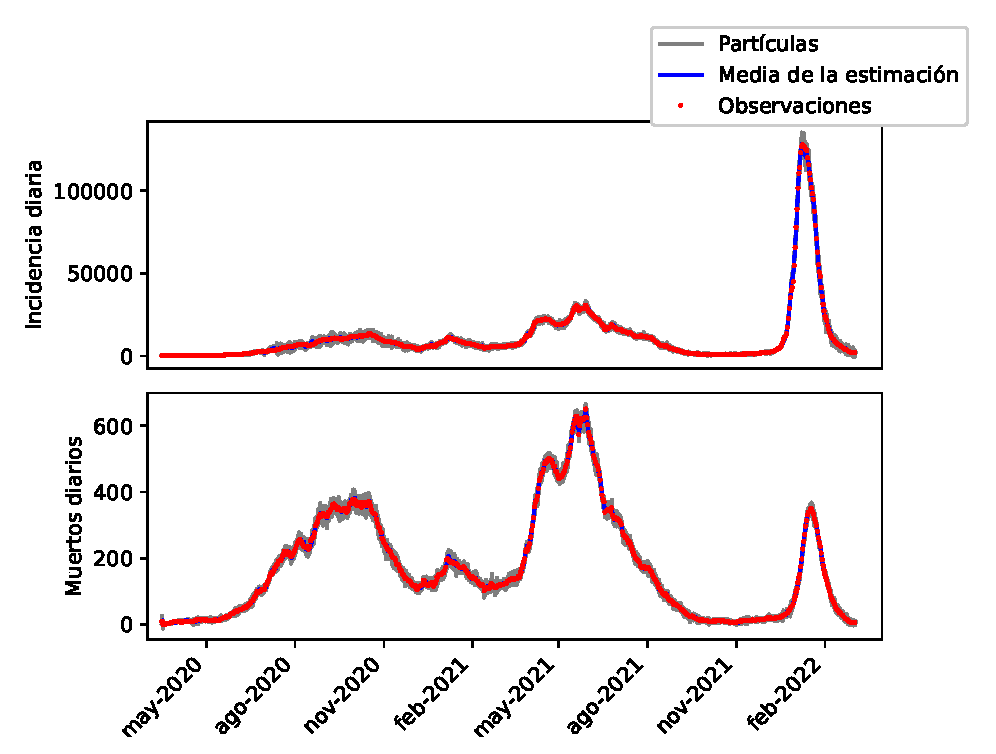
\includegraphics[width=0.75\textwidth]{figs/seird_online_em_aug_state_state_vars_arg_data.eps}
    \caption{Observaciones y estimaciones para los infectados diarios (incidencia diaria) y muertos diarios utilizando el modelo SEIRD sobre los datos de COVID-19 en Argentina}
    \label{fig:seird_vars_arg_data}
\end{figure}
\begin{figure}[h]
    \centering
    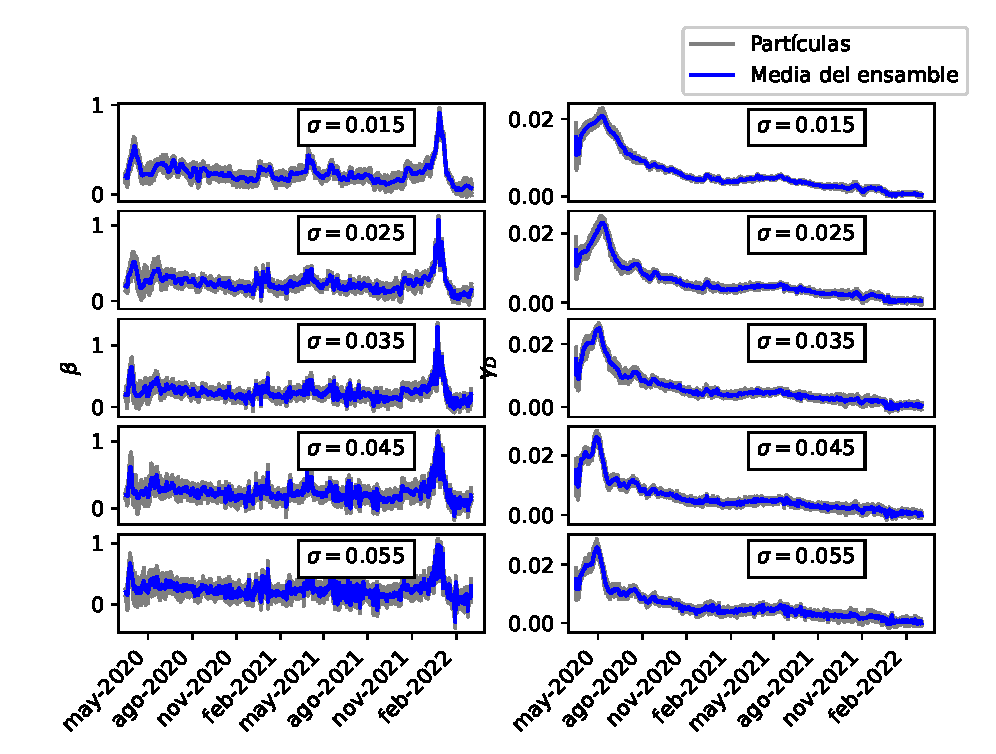
\includegraphics[width=0.75\textwidth]{figs/seird_online_em_aug_state_params_arg_data_sigmas.eps}
    \caption{Estimaciones de la tasa de infección $\beta$ y la tasa de fatalidad $\gamma_D$}
    \label{fig:seird_params_arg_data}
\end{figure}
\begin{figure}[h]
    \centering
    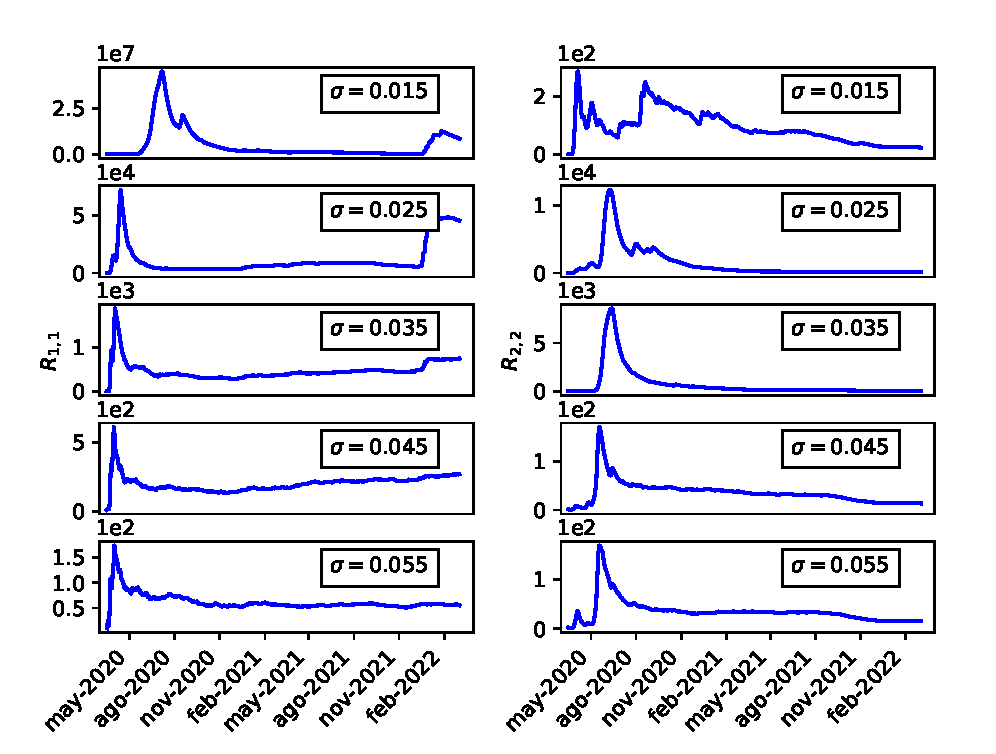
\includegraphics[width=0.75\textwidth]{figs/seird_online_em_aug_state_R_arg_data_sigmas.eps}
    \caption{Estimaciones del EM online de las varianzas de errores observacionales. Estas corresponden a los dos valores de la diagonal de las matrices de covarianzas $\v R_t$}
    \label{fig:seird_R_arg_data}
\end{figure}

\subsection{Discusión}

Diseñamos estos experimentos para mostrar la potencial viabilidad del EM \textit{online} para estimación de errores en sistemas de asimilación de datos sobre modelos epidemiológicos. Este aspecto es habitualmente pasado por alto en trabajos de inferecia mediante en este tipo de sistema. En el experimento con observaciones sintéticas, salvo por la parametrización que se calibra con estado aumentado, el modelo utilizado es el mismo que se usa para generar los datos. En el caso de tener datos reales no es posible especificar un modelo perfecto por lo que los parámetros en el estado aumentado cumplen el rol de calibrar otras posibles deficiencias del modelo. Los resultados obtenidos evidencian la interdependencia entre el error observacional y de modelo y como estos afectan la performace general de las estimaciones que produce el sistema. Una posibilidad es incorporar error de modelo aditivo y estimar su matriz de covarianza $\v Q_t$ con el EM \textit{online} y de hecho algunos experimentos preliminares sigieren que esto es posible. Además las varianzas de las caminatas aleatorias en el estado aumentado podrían potencialmente ser estimadas de manera adaptativa como parte de la matriz $\v Q_t$. Otra posibilidad más sencilla para dar cuenta del error de modelo es la utilización de un factor de inflación en el ensamble (ver Sección \ref{sec:enkf}).

\chapter{Asimilación de datos en modelos basados en agentes}

\section{Modelos basados en agentes}

A diferencia de los modelos de predeicción con ecuaciones diferenciales, los modelos basados en agentes (conocidos como ABMs por sus siglas en inglés) se basan en un paradigma diferente. Estos modelan de manera explícita las características y comportamiento de individuos o agentes que interactúan. El comportamiento conjunto de la población de agentes se utiliza como modelo de un sistema complejo \citep{Bonabeau2002}. Incluso reglas de interacción simples pueden resultar en que los agentes se organicen de manera autónoma y que el comportamiento colectivo de la población emerja de manera \textit{bottom-up} desde la escala micro del modelado de los individuos \citep{Helbing2012}. En general, los ABMs requieren una gran capacidad computacional ya que las poblaciones de agentes pueden ser muy grandes. Actualmente es factible utilizarlos de manera operacional y existen ejemplos de su aplicación en epidemiología, ecología, economía y sociología \citep{Vynnycky2010, Grimm2005, Tesfatsion2006, Epstein1996}.

Los modelos de agentes tienen dos componentes que los describen: 
\begin{enumerate}
    \item Las descripciones de los agentes
    \item Las reglas de comportamiento e interacción
\end{enumerate}
Los agentes pueden ser vistos como un tipo de dato con diferentes campos de manera que cada individuo se define por el valor de estos atributos. Para completar al modelo se agrega el comportamiento e interacción de los agentes, en general mediante reglas que pueden contener componentes estocásticos. Las acciones que realicen los individuos baje estas disposiciones provocarán cambios en los valores de sus atributos. En principio estos atributos pueden ser cualquier tipo de dato, de manera que los agentes pueden ser programados como tipos de datos compuestos (como estructuras en C) o incluso a través de clases en lenguajes orientados a objetos. Por ejemplo, se pueden usar números reales para representar coordenadas espaciales, variables categóricas para clases sociales, números enteros para edades, etc.

Para un modelar la dispersión de una enfermedad es apropiado construir ABMs epidemiológicos tomando una población de agentes en el que cada uno de ellos representa a una persona (o individuo susceptible a contraer y/o transmitir la enfermedad) \citep{Roche2011}. Utilizando variables categóricas se puede etiquetar a cada agente con su status o categoría epidemiológica (susceptible, infectado, etc.) y estas etiquetas pueden ser cambiadas cuando existe un contacto infeccioso o a medida que la enfermedad se desarolla en el tiempo. El modelado de los contactos entre agentes admite múltiples representaciones, se pueden hacer mezclas al azar, a través de grupos, con redes de contactos o modelando explícitamente la movilidad de los agentes en el espacio. El uso de ABMs para epidemiología tiene la virtud de que permite modelar de una manera explícita, y con gran detalle, características relevantes del sistema que suceden en la micro-escala de la intereacción entre individuos. Por ejemplo, la disminución de la inmunidad puede ser representada en cada individuo a través de un atributo. Es posible modelar de manera natural medidas de control como cuarentenas, reastreo de contactos o efectos de vacunación \cite{Silva2020}. Muchos modelos de ecuaciones diferenciales asumen que dentro de cada compartimento la mezcla entre individuos es homogénea; para ABMs epidemiológicos, al disponer de caracterizaciones de cada individuo, es posible obtener patrones de interacción mas ricos a través de redes de contacto o el mecanismo que resulte más conveniente. De esta manera se pueden capturar efectos difíciles de representar con modelos de ecuaciones diferenciales. A pesar de disponer de información de cada agente, en la simulación con ABMs el interés está en el comportamiento global del sistema. Se suele contar con una función que de alguna manera resuma al estado de la población como un todo a través de un conjunto de variables que llamaremos variables agregadas. En general, si tenemos que la población de agentes es $A$, llamaremos $\v x$ a las variables agregadas y $\phi$ a la función sintetizante que realiza el mapeo, de manera que:
\begin{align}
    \phi (A) = \v x
\end{align}
El comportamiento de las variables agregadas emergerá del comportamiento a nivel individual del ABM. En el caso de modelos epidemiológicos es razonable, por ejemplo, utilizar como resumen el conteo de la cantidad de individuos en cada categoría para saber cuantos susceptibles, infectados, recuperados, etc. hay.

Con el surgimiento de la pandemia de COVID-19 se han desarrollado una gran diversidad de ABMs. Algunos de estos incorporan, entre otras características, estructura de edades y redes de contactos a través de escuelas, casas, lugares de trabajo que permiten modelar de manera más realista las mezclas que dan lugar a los contacios \citep{Kerr2020,Flaxman2020,Simoy2021}. Además de que el aumento de la capacidad de cómputo hace más viable la utilización de ABMs, el gran caudal de datos recolectados a nivel individual a través de dispositivos electrónicos es otro gran aliciente para el incremento en su popularidad. En \cite{Aleta2020} se utilizan datos demográficos y de movilidad para construir las redes de contactos y distribución de hogares en un ABM que permite evaluar los efectos de las intervenciones no-farmacéuticas.

A pesar de la flexibilidad y expresividad que permite el modelado mediante agentes, sigue siendo necesario calibrarlos adecuadamente. En general, el aumento en complejidad viene acompañado de un aumento en el número de parámetros, los cuales no siempre son especificables a través del conocimento que se tenga sobre el sistema. Ha habido avances en el desarrollo de técnicas de inferencia para estimar parámetros en ABMs utilizando observaciones sobretodo orientados a la maximización de la verosimilitud. En particular en \cite{Hooten2020} se discuten una variedad de métodos para maximizar aproximaciones de la verosimilitud usando cómputo bayesiano aproximado (o ABM por \textit{Approximate Bayesian Computation}) junto con técnicas de MCMC (\textit{Markov Chain Monte Carlo}).

Como los ABMs se enmarcan en un contexto de sistemas con evolución temporal parcialmente observados, es posible pensar que la caja de herramientas provista por la asimilación de datos secuencial tiene potencial para realizar las tareas de inferencia. Un trabajo pionero en esta dirección es \cite{Ward2016} en el que se utiliza el EnKF para asimilar datos de cámaras de pisadas en calles Leeds con un modelo de agentes para estudiar el comportamiento del tráfico peatonal. A pesar de obtener resultados satisfactorios, se señala la dificultad asociada a la sensiblidad respecto a parámetros del modelo y la necesidad optimizar el código para modelos de gran tamaño. Como mencionamos anteriormente, el interés no necesariamente está puesto en estado de cada individuo sino en el estado global del sistema o deun conjunto de variables que den una descripción de la población de agentes que se considere relevante. Además, a pesar de que el estado a la escala microscópica determina de manera total al sistema y que el objetivo de la inferencia fuera, idealmente, representar esta escala de la manera más precisa posible, sucede que usualmente las observaciones que se tienen del sistema son de las varables sintetizantes, es decir de la escala macroscópica. Es decir, las observaciones pueden no tener suficiente ``resolución'' como para que se pueda determinar el estado de los atributos de cada agente. Nuestra propuesta, publicada en \cite{Cocucci2022}, es la de asimilar datos sobre las variables agregadas mediante técnicas basadas en ensambles. El mapeo de la escala microscópica a macroscópica está dado por la función sintetizante $\phi$ pero no tenemos una representación para su inversa. De hecho $\phi$ puede no ser inyectiva y por lo tanto no-invertible: muchas configuraciones de los agentes pueden resultar en el mismo estado de las variables agregadas. Esta situación debe considerarse para hacer un emparejamiento entre los estados macroscópicos observados y el estado de los atributos de los individuos. En este capítulo presentamos un esquema general de aplicación de métodos de asimilación de datos por ensambles para ABMs y dos implementaciones particulares para un ABM epidemiológico que también especificamos a continuación.

\section{Modelo epiABM} \label{sec:epi_abm}

Aquí especificamos un ABM epidemiológico diseñado para modelar la dinámica de contagio de enfermedades infecciosas, en particular para el COVID-19 y que denominaremos epiABM. Este es un modelo sencillo para evaluar el rendimiento de la metodología para aplicar asimilación de datos por ensambles en ABMs y no tiene el propósito de ser un modelo para realizar predicciones o asesorar en toma de decisiones.

El estado de salud de cada agente está descripto por una etiqueta para representar una entre siete categorías. Tenemos a los susceptibles a contraer la enfermedad ($S$), los expuestos a la enfermedad pero que aún no son infecciosos debido a que el virus está incubando ($E$). Después de considerarse expuestos pasan a una de dos posibles clases de infecciosos. Los infectados leves ($I_M$) son los que desarrollan una sintomatología que no requiere hospitalización y que eventualmente se recuperan. Los infectados graves ($I_S$) son los que requerirán hospitalización. Por su parte, los hospitalizados pueden recuperarse o morir. La categoría $R$ denomina a los recuperados y la $D$ a los muertos. Asumimos que los recuperados adquieren inmunidad permanente, lo cual no es una suposición realista para simulaciones a largo plaze de COVID-19 puesto que las reinfecciones son posibles. El diagrama de la figura \ref{dia:epi_abm} representa de manera esquemática la progresión de la enfermedad a través de estos estadíos.

\begin{figure}
    \begin{center}
        \tikzstyle{block} = [rectangle, draw, fill=blue!20, 
        text width=4em, text centered, rounded corners, minimum height=3em]
        \tikzset{line/.style={draw, very thick, color=black!100, -latex'}}
        \centering
        \begin{tikzpicture}[node distance = 2cm, auto]
            \tikzstyle{block} = [rectangle, draw, fill=blue!20, 
            text width=2em, text centered, rounded corners, minimum height=3em]
            
            % Place nodes
            \node [block] (S) {$S$};
            \node [block, right of=S] (E) {$E$};
            \node [block, above right = 0.05cm and 1cm of E] (IM) {$I_M$};
            \node [block, below right = 0.05cm and 1cm of E] (IS) {$I_S$};
            \node [block, right of=IS] (H) {$H$};
            \node [block, right of=H] (D) {$D$};
            \node [block] (R) at (IM-|D) {$R$};
            
            % Draw edges
            \draw[line] (S) -- (E);
            \draw[line] (E) |- node [below] {$q_S$} (IS);
            \draw[line] (E) |- node [above] {$1-q_S$} (IM);
            \draw[line] (IM) -- (R);
            \draw[line] (IS) -- (H);
            \draw[line] (H) -- node [above] {$q_D$} (D);
            \draw[line] (H) -- node [left = 0.01cm] {$1-q_D$} (R);
        \end{tikzpicture}
    \end{center}
    \caption{Diagrama de las categorías epidemiológicas dee modelo epiABM.}
    \label{dia:epi_abm}
\end{figure}

En cada paso temporal, que consideraremos de un día, cada agente tendrá un número de contactos muestreado de una distribución Poisson de parámetro $\lambda$. Los agentes susceptibles podrán resultar infectados por un contacto con un agente infeccioso. El tiempo de permanencia de un agente en las categorías ``intermedias'' ($E$, $I_M$, $I_S$, $H$) está muestreado de una distribución Gamma. Si nombramos a este tiempo $\tau_c$ con $c \in \{E, I_S, I_M, H\}$ entonces $\tau_c \sim \Gamma(k_c, \theta_c)$ donde $k_c$ y $\theta_c$ son los parámetros de forma y escala respectivamente. Con esta parametrización, la media $\mu_c$ y la varianza $\sigma^2_c$ cumplen con las relaciones $\mu_c = k_c \theta_c$ y $\sigma^2_c = k_c \theta_c^2$. El tiempo $\tau_c$ es muestreado para cada agente cuando este entra a la categoría $c$ y cuando este tiempo expira, el agente pasa a la siguiente categoría. Cuando un agente sale de la categoría $E$, tiene una probabilidad $q_S$ de tener una enfermedad severa y $q_M = 1 - q_S$ de que su enfermedad sea leve. Análogamente, los hospitalizados tienen una probabilidad $q_D$ de morir y $q_R = 1 - q_D$ de recuperarse.

Además de la estructura dada por el estatus epdemiológico, incluímos información demográfica y geográfca. El modelo considera una ciudad dividida en $N_{loc}$ comunas. Cada agente vive en una casa (solo o con otros agentes) en una determinada comuna. El tamaño de los hogares sigue una distribución determinada por el vector de probabilidades $p_H$ en el cual la $i$-ésima entrada determina la probabilidad de que un hogar tenga $i$ miembros. Los contactos entre agentes pueden entonces ser definidos en base a esta estructura sencilla. Diferenciaremos entre contactos domésticos y casuales. Cada uno de los contactos diarios de los agentes tiene una probablilidad $q_C$ de ser casual y $1 - q_C$ de ser doméstico. Los contactos domésticos se dan solamente entre miembros de un mismo hogar mientras que los casuales pueden ser, potencialmente con cualquier otro agente. Llamamos $\beta_D$ (respectivamente $\beta_C$) a la probabilidad de que un contacto doméstico (respectivamente casual) sea infeccioso. De esta manera podemos escribir una expresión para el valor esperado para la probabilidad de infección global como $\beta = q_C \beta_C + (1 - q_C) \beta_D$. Por su parte, los contactos casuales van a estar mediados por la conectividad entre los diferentes barrios. Llamaremos $C_{ij}$ a la probabilidad de que un contacto casual de un agente del barrio $j$ se de con un agente del barrio $i$. Esto resulta en una matriz $C$ de tamaño $N_{loc} \times N_{loc}$ que nombraremos matriz de contacto. Los elementos de la diagonal corresponden a la probabilidad de que un contacto casual se de entre habitantes del mismo barrio mientras que los elementos fuera de ella tienen que ver con los contactos entre habitantes de barrios distintos. La matriz $C$ codifica entonces la movilidad entre barrios que a su vez se relaciona a las actividades sociales y laborales de la ciudad. El diseño de esta matriz puede incluír diferentes características de la estructura social y geográfica de la ciudad. Por ejemplo, sería esperable que los agentes transiten con más frecuencia su propio barrio, lo que implicaría valores más altos en los elementos de la diagonal y más pequeños por fuera de esta. Por otro lado, en caso de tener un barrio con más tránsito, por ejemplo un barrio céntrico, los valores correspondientes por fuera de la diagonal serían mayores que en el caso de un barrio menos visitado. Para este trabajo consideraremos que $C$ está fija en el tiempo pero existe la posibilidad de diseñar esta matriz con mayor detalle: por ejemplo se podría ajustar utilizando datos de movilidad que cambien en el tiempo para contemplar cambios que afectarían al contacto entre personas o incluso para incluír los efectos de medidas de control como cuarentenas o restricciones de movilidad. Aquí utilizamos expresiones sencillas para la matriz de contactos porque el objetivo principal es el de la evaluación de la metodología propuesta para asimilar datos en ABMs. Una parametrización por defecto para el modelo se especifica en el Apéndice \ref{appendix:epi_abm_default_params}.

El modelo puede ser extendido añadiendo más atributos a los agentes o representando con mayor detalle los patrones de contacto entre personas. Por ejemplo, sería posible incorporar edades o perfiles sociales para enriquecer la configuración de relaciones entre contactos que sean relevantes para la descripción de la dispersión de la enfermedad. Añadir eventos sociales de gran concurrencia, como por ejemplo lugares de trabajo o escuelas puede ser útil para el modelado de los fenómenos de dispersión masiva (conocidos como eventos \textit{superspreader}). También es posible incluir otras características como las campañas de vacunación o el sugrimiento de nuevas cepas del virus. Incorporando campos a la descripción del estado de los agentes se puede determinar si están vacunados, cuantas dosis recibieron, etc. Por otro lado, se puede indicar con qué variante del virus se contagiaron los agentes infectados.

El ABM subdivide al total de agentes en subpoblaciones de acuerdo a categorías epidemiológicas de manera similar a modelos compartimentales de ecuaciones diferenciales. Sin embargo los ABMs no pueden ser descriptos de manera directa con ecuaciones diferenciales. Cuando el número de agentes es grande las variables agregadas pueden suavizar el efecto de las componentes estocásticas (por ejemplo de los tiempos muestreados de distribuciones Gamma) y como resultado pueden llegar a ser reproducibles con modelos de ecuaciones diferenciales. Los ABMs tienen características, tal como el comportamiento de tener agentes que residen en hogares y con tasas de infección diferenciadas entre contactos domésticos y casuales, para las cuales no está claro como se podrían traducir a un modelo basado en ecuaciones. El modelado a nivel microscópico de los ABMs puede tener consecuencias en la gran escala que pueden no ser fáciles de predecir. A pesar de esto, es importante destacar que los ABMs pueden tener un alto costo computacional lo cual a motivado el uso de modelos de ecuaciones que actúan como sustitutos de un ABM y que pueden ser utilizados para realizar inferencia con bajo costo computacional \citep{Hooten2020}.

\section{Asimilación de datos en ABMs}

Para aplicar técnicas de asimilación de datos a ABMs es necesario entender primero que el estado propiamente dicho de un sistema de agentes en un instante de tiempo $t$ está dado por el valor de los atributos de cada uno de los agentes que componen la población. El principio no es conveniente aplicar asimiliación de datos en un espacio de estas características porque, por un lado, la cantidad de variables es enorme (igual a la cantiad de agentes multiplicado por la cantidad de atributos) y por otro lado muchos de los atributos pueden no ser valores numéricos. Es posible aplicar filtros de partículas sobre espacios con variables categóricas pero apuntamos a usar el EnKF el cual trabaja sobre espacios de números reales. Incluso de ser factible asimilar datos en el espacio dado por los atributos de los agentes es probable que el interés principal esté en la inferencia sobre las variables agregadas. En el caso del modelo epiABM las variables agregadas estarán dadas por la cantidad de agentes con determinados atributos (por ejemplo estado epidemiológico y comuna). Estos valores son enteros pero al ser lo suficientemente grandes pueden ser considerados como en un espacio continuo por el EnKF. Además de este punto notemos que en general, las observvaciones sobre el sistema serán sobre las variables agregadas, por lo que serán más informativas sobre el valor de estas cantidades y por lo tanto es más directo intentar la inferencia sobre el espacio que estas determinan.

Llamaremos al conjunto de valores de atributos del $k$-ésimo agente en una población a tiempo $t$ como $A_{k, t}$. A su vez, al conjunto de estos valores para toda la población de agentes la llameremos $A_t = \{ A_{k, t} \}_{k=1}^{N_a}$, donde $N_a$ es el número total de individuos. Debido a que nuestro enfoque apunta a utilizar técnicas basadas en muestras debemos considerar que tenemos no una población sino un ensamble de tamaño $N_p$ de poblaciones de tamaño $N_a$. Este ensamble puede ser representado como $\{ A_{t}^{(j)} \}_{j=1}^{N_p}$. Por su parte, el proceso de asimilación de datos se dará sobre las variables agregadas, o macroscópicas, $\v x_t$. Estas se pueden obtener de una población de agentes $A_t$ mediante la aplicación de la función sintentizante, de manera que tenemos $\v x_t = \phi (A_t)$. De esta manera tenemos el ABM para evolucionar temporalmente a la población de agentes de $A_t$ a $A_{t+1}$ y mediante $\phi$ podemos obtener las variables agregadas $\v x_{t+1}$. El inconveniente es que la función $\phi$ no será en general inyectiva y por lo tanto no será invertible, es decir que muchas configuraciones distintas de la población de agentes pueden dar las mismas variables agregadas. La técnica de asimilación de datos actualiza las variables sobre las que actúa cuando incorpora la información de una observación. En nuestro caso se actualizará a $\v x$ pero como $\phi$ no es invertible no tenemos una manera explícita de dar cuenta de este cambio sobre la población de agentes. Es importante notar que tanto para el EnKF como para el filtro de partículas el modelo es tratado como una caja negra por lo que estas técnicas actuarán ignorando por completo la existencia del mapeo $\phi$.

Al tiempo $t$ supongamos que tenemos un ensamble $\{ A_{t}^{f(j)} \}_{j=1}^{N_p}$. Cada miembro del ensamble $A_{t}^{f(j)}$ representa una población de agentes donde el supraíndice $f$ indica que la muestra es de un \textit{forecast}. Para obtener un pronóstico de las variables de estado simplemente debemos aplicar $\phi$ a cada $A_{t}^{f(j)}$ y de esa manera conseguimos el ensamble $\{ \v x_{t}^{f(j)} \}_{j=1}^{N_p}$. Utilizando este pronóstico en combinación con la observación $\v y_t$ obtenemos, mediante la actualización de la técnica de asimilación de datos, un ensamble de análisis $\{ \v x_{t}^{a(j)} \}_{j=1}^{N_p}$. En este punto, en un esquema de asimilación de datos por ensambles tradicional utilizaríamos el modelo para evolucionar $\{ \v x_{t}^{a(j)} \}_{j=1}^{N_p}$ en $\{ \v x_{t+1}^{f(j)} \}_{j=1}^{N_p}$, es decir que con las variables de estado de análisis a tiempo $t$ obtendríamos un pronóstico a tiempo $t+1$. Pero el ABM no puede transformar directamente $\v x_t$ en $\v x_{t+1}$ sino que evoluciona a $A_t$ en $A_{t+1}$. Necesitamos entonces una representación de agentes $A_{t}^{a(j)}$ de las variables $\v x_{t}^{a(j)}$. Esta población de agentes puede entonces ser usada por el ABM para obtener las poblaciones de agente de pronóstico $\{ A_{t+1}^{f(j)} \}_{j=1}^{N_p}$ para el tiempo siguiente y retomar la iteración pronóstico-análisis. En la Figura \ref{dia:ensemble_DA_ABM} se sintetiza este procedimiento general. El ingrediente faltante entonces es el ajuste de la población de agentes a las variables agregadas actualizadas mediante la información observacional. Para esto discutiremos dos metodologías distintas para el caso del epiABM

\begin{figure}
\captionsetup{width=0.5\textwidth}
\begin{center}
\tikzset{line/.style={draw, very thick, color=black!100, -latex'}}
\begin{tikzpicture}[node distance = 3cm, auto]
    \tikzstyle{block} = [rectangle, draw, fill=blue!20, 
    text width=5em, text centered, rounded corners, minimum height=3em]
    \tikzstyle{observation} = [circle, draw, fill=blue!20, 
    text width=1.5em, text centered, rounded corners, minimum height=1em]

    % Place nodes
    \node [block] (Af) {$\{A_t^f\}_{j=1}^{N_p}$};
    \node [block, below = 1cm of Af] (xf) {$\{ \v x_t^f\}_{j=1}^{N_p}$};
    \node [observation, below right=0.5cm and -0.5cm of xf] (y) {$\v y_t$};
    \node [block, below of=xf] (xa) {$\{ \v x_t^a\}_{j=1}^{N_p}$};
    \node [block, below = 1cm of xa] (Aa) {$\{A_t^a\}_{j=1}^{N_p}$};

    \node [block, right=2cm of Af] (Af1) {$\{A_{t+1}^f\}_{j=1}^{N_p}$};
    \node [block, below = 1cm of Af1] (xf1) {$\{ \v x_{t+1}^f\}_{j=1}^{N_p}$};
    \node [observation, below left=0.5cm and -0.5cm of xf1] (y1) {$\v y_{t+1}$};
    \node [block, below of=xf1] (xa1) {$\{ \v x_{t+1}^a\}_{j=1}^{N_p}$};
    \node [block, below = 1cm of xa1] (Aa1) {$\{A_{t+1}^a\}_{j=1}^{N_p}$};

    \coordinate[below left = 1cm and 1cm of Aa] (aux);
    \coordinate[below right = 1cm and 1cm of Aa1] (aux1);
    \coordinate[left = 0.5cm of Af] (prev);
    \coordinate[right = 0.5cm of Aa1] (follow);

    % Draw edges
    \draw[line] (Af) -- node [left] {$\phi$}  (xf);
    \draw[line] (xf) -- node [left, text width=2cm, align=right] {Asimilación}  (xa);
    \draw[line] (xa) -- node [left, text width=3cm, align=right] {Ajuste de\\ agentes}  (Aa);
    \draw[line] (y) -- ($(xa.north) + (0.25cm, 0cm)$);

    \draw[line] (Aa.north east) -- node [sloped, below, midway] {ABM} (Af1.south west);

    \draw[line] (Af1) -- node [right] {$\phi$} (xf1);
    \draw[line] (xf1) -- node [right, text width=2cm, align=left] {Asimilación} (xa1);
    \draw[line] (xa1) -- node [right, text width=3cm, align=left] {Ajuste de\\ agentes} (Aa1);
    \draw[line] (y1) -- ($(xa1.north) - (0.25cm, 0cm)$);

    \draw[line] (aux) -- node {Tiempo} (aux1);
    \path (prev) -- node[auto=false]{\ldots} (Af);
    \path (Aa1) -- node[auto=false]{\ldots} (follow);

\end{tikzpicture}
\caption{Esquema general de asimilación de datos por ensambles para ABMs}
\label{dia:ensemble_DA_ABM}
\end{center}
\end{figure}

\subsection{Metodologías de ajuste de agentes}

Para aplicar el esquema propuesto es necesario entonces construir una población de agentes consistente con el estado de las variables macro una vez que estas fueron actualizadas por el sistema de asimilación de datos. El problema es que para cada $j = 1, ..., N_p$ tendremos una discordancia entre las variables de estado de la población d agentes que tenemos como pronóstico $\v x_t^{f(j)} = \phi (A_t^{f(j)})$ y el valor corregido para las variables agregadas actualizadas $\v x_t^{a(j)}$. Nuestra aproximación al problema es utilizar la misma población que se tenía como pronónstico, es decir $\{A_t^{f(j)}\}_{j=1}^{N_p}$, y hacer los cambios necesarios para obtener $\{A_t^{a(j)}\}_{j=1}^{N_p}$ consistentes con $\{\v x_t^{a(j)}\}_{j=1}^{N_p}$. Esto está inspirado en que los agentes del análisis son una corrección de los del pronóstico. Mientras mejor sea el pronóstico, menos agentes deberán ser modificados. Sin embargo, la estructura interna de los agentes puede ser muy compleja, con muchos atributos más allá de los considerados por la función sintetizante $\phi$. Si estos atrubutos podrán ser ajustados de manera realista dependerá del ABM y de cuánto de la estructura interna de los agentes se ve representada en las variables del macro-estado.

Para el modelo epiABM presentado en la Sección \ref{sec:epi_abm} consideraremos dos metodologías distintas para corregir las poblaciones de agentes. Nuestra función sintetizante $\phi$ simplemente contará la cantidad de agentes en cada categoría epidemiológica en cada barrio por separado. Como tenemos $N_x = 7$ categorías epidemiológicas distintas y $N_{loc}$ barrios, la dimensión de estas variables será $7 N_{loc}$. Para la primera consideraremos las categorías donde ``sobran'' agentes (comparando con el valor deseado, es decir el análisis de las variables agregadas) y los redistribuiremos en las categorías que muestran un déficit de agentes hasta lograr el objetivo de coincidir con los valores de $\v x_t^{a(j)}$. Los agentes se seleccionan al azar (de las categorías correspondientes) y por ello llamamos a este método redistribución aleatorizada. El cambio de categoría de agentes se hace mediante un cambio de etiquetas y el procedimiento se repite de manera independiente en cada barrio. Pero no solo es necesario realizar cambios en las categorías epidemiológicas sino que hay otros atributos que deben ser atendidos. Por ejemplo, cada agente en las categorías $E$, $I_M$, $I_S$ o $H$ posee un contador que indica cuanto tiempo le queda para pasar a la categoría siguiente. Estos contadores son originalmente muestreados de distribuciones Gamma, como se especificó en la Sección \ref{sec:epi_abm}. Entonces, cuando un agente es introducido por la actualización a una de estas categorías se debe dar un valor a este contador. Nuestra elección es muestrear el valor al azar de los agentes que ya están en dicha categoría para intentar preservar la distribución de ese valor dentro de la población. Aunque esta metodología es particular para la aplicación sobre nuestro modelo se pueden hacer implementaciones similares en general siempre y cuando tengamos un conocimiento a priori sobre la distribución del valor del atributo a través de la población de agentes. La idea del método es ser lo menos intrusivo posible con la población de agentes original y en este sentido la cantidad de agentes que se modifica es la mínima posible para lograr la coherencia con las variables agregadas.

La segunda metodología de ajuste de agentes no apunta a minimizar la cantidad de agentes modificados sino a intentar preservar la historia de cada agente individualmente. Para seleccionar los agentes a ser modificados intentaremos escoger aquellos que más probablemente tengan que cambiar de categoría según un criterio epidemiológico. Los cambios sólo se darán entonces entre categorías adyacentes la cadena de progresión de la enfermedad representada en el diagrama de la Figura \ref{dia:epi_abm}. Las correcciones comenzarán en las últimas etapas ($R$ y $D$) y se avanzará hacia atrás hasta llegar a $S$. Además, la selección de los agentes que cambiarán de categoría no será al azar. Si un cambio debe ser hecho en la dirección del flujo del diagrama se elegirán los agentes que hayan pasado más tiempo en su categoría actual como los que más probablemente deban proseguir a la siguiente para hacer la corrección. De manera análoga, si un cambio debe ser hecho en el sentido contrario al flujo del diagrama se elegirán los agentes que hayan pasado menos tiempo en su actual categoría y se los retornará a la categoría anterior. La idea es preservar en lo posible las trayectorias individuales de cada agente. Para los cambios entre susceptibles y expuestos usaremos un criterio distinto, porque que un agente haya estado mucho tiempo como susceptible no significa que necesariamente sea más propenso a infectarse. En ese caso el criterio es mover de susceptibles a expuestos los agentes que más contactos riesgosos hayan tenido (es decir contactos con agentes infecciosos, los cuales no resultan siempre en infección). En la dirección opuesta, es decir para mover agentes de la cateoría de expuestos a susceptibles se sigue usando el criterio de días de permanencia en la clase. Cada vez que un agente cambia de categoría el contador correspondiente se reinicia muestreando valores de los contadores de los agentes que ya estaban en la categoría donde fue reasignado. Este proceso se repite para cada barrio de manera independiente al igual que en la redistribución aleatorizada. Llamamos redistribución con cascada hacia atrás a la metodología resultante. Una desventaja del método es que cuando seleccionamos a los agentes con más permanencia en una categoría estamos truncando las colas de la distribución de ese atributo.

\section{Evaluación experimental}

Realizamos una evaluación experimental de los métodos propuestos acoplados con el EnKF en el modelo epiABM. Primero usamos observaciones sintéticas de manera que el estado verdadero del que son muestreadas las observaciones es generado con el modelo y está disponible para ser comparado con las estimaciones. Luego utilizamos datos de casos de COVID-19 en la Ciudad Autónoma de Buenos Aires (CABA), Argentina. 

Como mencionamos anteriormente, la cantidad de variables de estado está dada por $N_x N_{loc}$ donde $N_x$ es la cantidad de categorías epidemiológicas y $N_{loc}$ la cantidad de barrios o comunas. En realidad, a estas variables de estado también se le agregan posiblemente los parámetros que se esimen mediante estado aumentado. A no ser que se mencione explícitamente utilizamos la parametrización por defecto especificada en el Apéndice \ref{appendix:epi_abm_default_params}.

En los experimentos consideramos como variables observadas a los casos acumulados y muertes acumuladas, ambas desagregadas por barrio. Los casos acumulados pueden ser computados como la suma de $I_M$, $I_S$, $H$, $R$, $D$ en cada barrio. Al error en las observaciones lo suponemos Gaussiano e insesgado com varianza proporcional a la variable observada correspondiente. Los coeficientes de proporcionalidad los nombramos como $k_C$ y $k_D$ respectivamente.

La versión del EnKF que utilizamos es la estocástica o con observaciones perturbadas \citep{Burgers1998}. Aunque es usual utilizar algún tipo de inflación multiplicativa o aditiva en este tipo de métodos para evitar el colapso del ensamble (ver Sección \ref{sec:enkf}), pudimos detectar en experimentos preliminares que esto no se hace necesario debido a que la estocasticidad intrínseca del modelo mantiene a las trayecrotias del ensamble con suficiente dispersión. Por otra parte, la variabilidad inicial del ensamble está dada por muestreo aleatorio en la inicialización de los atributos de los agentes.

Realizamos un análisis de sensitividad en un experimento sintético para determinar un tamaño de ensamble adecuado y obtuvimos que con ensambles mayores a 50 miembros no se obtenía una mejora significativa en el error cuadrático medio (RMSE). Por otro lado, la varianza se estabiliza recién con ensambles de 100 miembros. Tomamos entonces 100 miembros de ensamble como el tamaño para los experimentos sintéticos. Para los experimentos con datos reales no podemos hacer una evaluación de la sensitividad pero como tenemos aproximadamente el cuádruple de variables de estado (porque tenemos más cantidad de barrios) consideramos 400 miembros de ensamble. En ambos casos, incrementar el tamaño del ensamble no resulta en cambios detectables en los resultados.

\subsection{Observaciones sintéticas}

Hacemos aquí una evaluación experimental del métodos para distintas configuraciones simulando las observaciones. En la mayor parte de los experimentos, el modelo que se emplea para generar las observaciones es el mismo que se utiliza para realizar la inferencia, lo que permite comparar las trayectorias reales con las estimadas. Sin embargo en algunos casos consideramos parámetros desconocidos o incluso especificaciones distintas del modelo. Tomamos un total de $N_{loc} = 4$ barrios y usamos la siguiente matriz de contacto:
\begin{align*}
    C = 
    \begin{pmatrix}
        0.43 & 0.14 & 0.14 & 0.29 \\
        0.14 & 0.43 & 0.14 & 0.29 \\
        0.14 & 0.14 & 0.43 & 0.29 \\
        0.14 & 0.14 & 0.14 & 0.57 
    \end{pmatrix}.
\end{align*}
Consideramos que los agentes tienen contactos casuales con mayor probabilidad dentro de sus propios barrios, lo que explica que los valores en la diagonal sean mayores. Adicionalmente, el barrio con mayor indexación es considerado como un barrio más concurrido por lo que tenemos mayores valores en la última conlumna.

\subsubsection{Número de contactos variable}

El número de contactos que tiene un agente por día está codificado a través del parámetro $\lambda$. En este experimento consideramos que el valor real de este parámetro disminuye linealmente en el tiempo y en el sistema de inferencia lo estimamos mediante estado aumentado.

La Figura \ref{fig:abm_state_vars_moving_lambda} muestra los resultados de las variables de estado reales y estimadas por el EnKF. Se puede ver que el ensamble estima correctamente a las trayectorias reales. El ensamble que estima las muertes acumuladas tiene muy poca varianza, esto se debe a que esta variable es directamente observada y con un error observacional relativamente pequeño. El resto de las variables no son observadas y sus estimaciones se logran a través del uso de las correlaciones con las variables observadas que hace el EnKF. En la Figura \ref{fig:abm_moving_lambda} se grafican la trayectoria real y las del ensamble para $\lambda$. Las estimaciones capturan el cambio en el parámetro luego de un tiempo inicial de spin-up en que el sistema de asimilación sincroniza con las observaciones a medida que las incorpora. Alrededor del pico epidémico es cuando la varianza de las estimaciones es menor y luego de eso comienza a amplificarse. Esto se debe a que las observaciones son más informativas de $\lambda$ (a través de correlaciones) cuando el número de infecciones es mayor. A medida que el número de infecciones disminuye la incerteza en las estimaciones comienza a crecer. La media del ensamble inicial se elije adrede en un valor distinto al valor real inicial de $\lambda$ ya que el parámetro se supone desconocido. Por otro lado, consideramos una varianza inicial grande para que el ensamble pueda explorar mejor el espacio paramétrico. A medida que crece la correlación entre las variables observadas y el parámetro, esta varianza se comienza a encoger. En todos los casos se muestran los resultados para la redistribución aleatorizada pero estos son similares con la cascada hacia atrás.
\begin{figure}[h!]
    \centering
    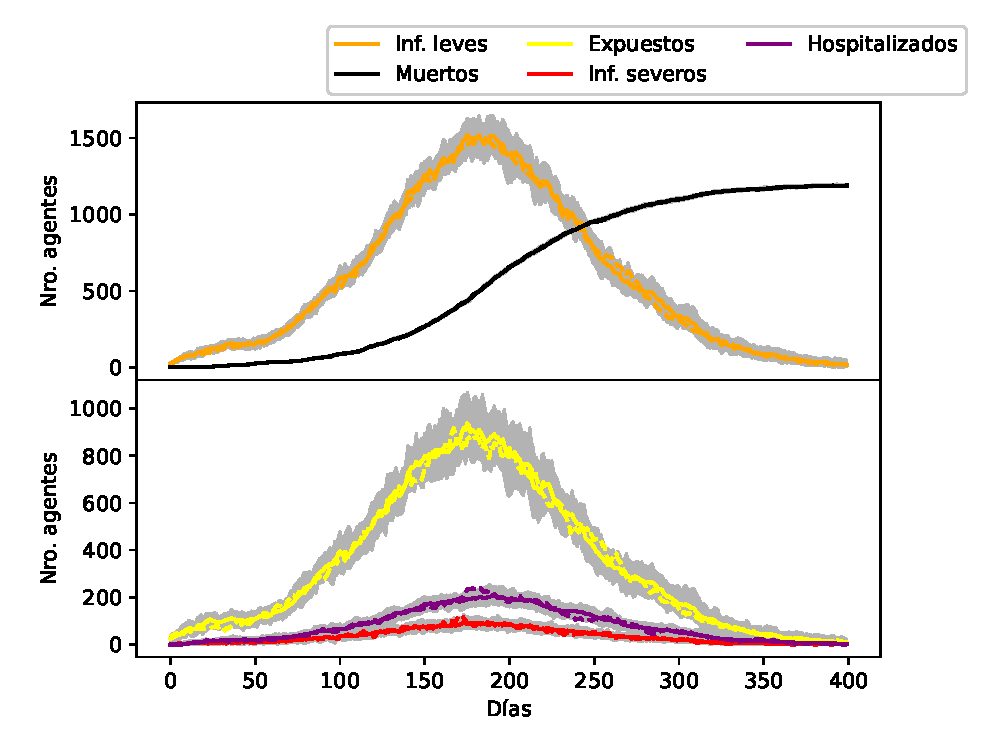
\includegraphics[width=0.75\textwidth]{abm_state_vars_moving_lambda.eps}
    \caption{}
    \label{fig:abm_state_vars_moving_lambda}
\end{figure}
\begin{figure}[h!]
    \centering
    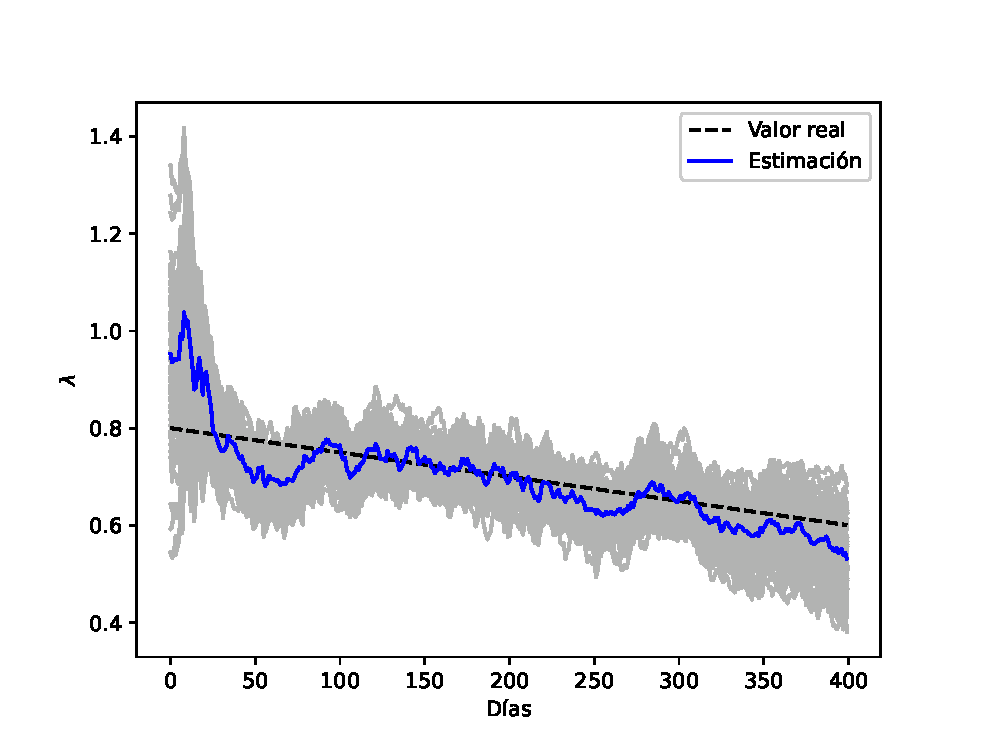
\includegraphics[width=0.75\textwidth]{abm_moving_lambda.eps}
    \caption{}
    \label{fig:abm_moving_lambda}
\end{figure}
\begin{figure}[h!]
    \centering
    \includegraphics[width=0.75\textwidth]{abm_housing_dist_moving_lambda.eps}
    \caption{}
    \label{fig:abm_housing_dist_moving_lambda}
\end{figure}

La estructura dada por la distribución de agentes en hogares no es informada de manera directa por las observaciones puesto que estas solo están diferenciadas por barrio. El sistema sin embargo mantiene una población de agentes por cada miembro de ensamble y es posible evaluar cómo se distribuyen las infecciones en los distintos tipos de hogares. Nuestra parametrización del modelo considera casas desde un solo habitante hasta un máximo de cinco. En cada día de asimilación computamos qué proporción de infectados corresponde a cada tamaño de hogar: los resultados se muestran en la Figura \ref{fig:abm_housing_dist_moving_lambda}. Cuando hay menos infecciones, es decir antes y después del pico epidémico las estimaciones tienen varianza más alta y son menos precisas mientras que durante el pico de infecciones la dispersión es mucho menor y las estimaciones más certeras. Podemos comparar la proporción de infectados en cada tipo de hogar con la proporción total de agentes en cada tio de hogar sin importar su estado epidemiológico. En casas más pequeñas la proporción estimada de infecciones es menor a la proporción de agentes residentes en ese tipo de hogar. Lo opuesto sucede en casas de mayor tamaño. Esto se debe a que debido a los contactos domésticos la infección se dispersa con mayor rapidez en hogares con más habitantes. A su vez, la proporción de infectados en hogares más grandes es mayor al comienzo de la epidemia y menor hacia el final porque son los hogares que más rápidamente se saturan de inmunes (por infectarse más rápidamente).

\subsubsection{Seguimiento de la microescala}

Realizamos un experimento en el que evalúamos, en distintos niveles de agrupamiento, qué cantidad de agentes coinciden en su estado epidemiológico,  comparando entre las estimaciones y la corrida real. El objetivo del experimento es comparar la evolución del estado en la micro-escala entre la población real de agentes y las de los miembros del ensamble. Contaremos la cantidad de agentes que tienen el mismo estado epidemiológico pero considerando diferentes agrupamientos de agentes. Cada agente tiene un número de identificación (id); la primera métrica consistirá en comparar el estado epidemoiológico de los agentes id por id. La segunda métrica consistirá en comparar casa por casa para chequear coincidencias. Para la tercera métrica agruparemos los agentes de acuerdo al tamaño de hogar en el que habitan. La última métrica agrupa agentes de acuerdo al tamaño de hogar y el barrio en que habitan. La única métrica que distingue agentes por su id es la primera, para el resto contamos las coincidencias simplemente contantdo la cantidad de agentes en la misma categoría epidemiológica. Utilizamos $N_{loc} = 4$ barrios y en lugar de utilizar un valor de $\lambda$ global consideramos un valor distinto para cada locación, de manera que tenemos un vector de $N_{loc}$ componentes $\lambda = (1.0, 0.8, 0.9, 0.7)$. 

La configuración inicial de los agentes para la corrida real y los miembros del ensamble es la misma por lo que al comienzo el porcentaje de coincidencias es 100\% para todas las métricas. Para evaluar el impacto de la asimilación  producimos además 100 simulaciones sin ningún tipo de asimilación para poder comparar los resultados. Estas darán diferentes resultados que la trayectoria real debido a la estocasticidad del modelo.

La Figura \ref{fig:abm_matchings} muestra los resultados para ambos métodos de ajuste de los agentes y para las simulaciones sin asimilación de datos. Cada panel muestra una de las métricas. La metodología de redistribución aleatorizada y de cascada hacia atrás producen resultados similares en todos los casos. Las trayectorias de las métricas para las corridas independientes tienen una gran dispersión mientras que cuando se asimilan datos estas están contenidas. Para las métricas de id de agentes y de casas, que son las que evalúan a una escala más microscópica, se puede ver que el porcentaje de coincidencias cae, se recupera un poco y finalmente se estabiliza tanto para las corridas con EnKF como para las simulaciones independientes. Estas últimas son ligeramente más consistentes con la corrida real en la primera etapa en que todas las métricas caen. Esto es posiblemente debido a que la metodología de ajuste debe modificar el estado de agentes para lograr la consistencia con las variables macroscópicas mientras que las simulaciones independientes mantienten en mayor medida la estructura inicial de la población de agentes.
\begin{figure}[h!]
    \centering
    \includegraphics[width=0.75\textwidth]{abm_matchings.pdf}
    \caption{}
    \label{fig:abm_matchings}
\end{figure}

En la escala de tamaños de hogares el EnKF mantiene un porcentaje alto de coincidencias (mayor al 90\% para ambas metodologías de ajuste). En cambio, las simulaciones independientes muestran una gran variabilidad. El resultado para la métrica que agrupa por tipo de hogar y barrio da resultados similares. Algunas de las trayectorias de las simulaciones independientes tendrán picos epidémicos que no coinciden con el de la trayectoria real por lo que es esperable que las métricas para estas corridas decrezcan. El porcentaje de coicidencias luego se recupera puesto que el tamaño final de la epidemia será similar para la corrida real y las simulaciones y la mayor parte de los agentes estará en la categoría de susceptibles o recuperados. Por su parte, para el EnKF tenemos un buen nivel de coincidencias para estas métricas debido a que al asimilar datos, las trayectorias del ensamble pueden detectar el pico epidémico y sincronizar con el estado real en esta escala. Es importante notar que las observaciones en estos experimentos están separadas por barrio pero no son explícitamente informativas respecto a las infecciones en distintos tamaños de hogar. Aún así el porcentaje de coincidencias es bastante alto para estas métricas. La proporción de coincidencias considerando ids de agentes o agrupando por casas particulares es similar usando asimilación de datos o no haciéndolo. Esto es posiblemente porque los ids de agentes o de casas no juegan un rol particular en las dinámicas de contagio. En cambio, el tipo de hogar sí tiene un efecto en la dispersión de la enfermedad y por lo tanto este es capturado por el EnKF.

\subsubsection{Estimación de casos no detectados}

Es esperable que los datos de infecciones de COVID-19 estén afectados por el subreporte de casos debido a que existen muchos casos muy leves o incluso asintomáticos. Para evaluar este escenario modificamos levemente nuestro modelo y consideramos que las infecciones leves tienen una posibilidad $q_A$ de ser asintomáticos y por lo tanto no ser reportados. Para el experimento utilizamos una configuración similar a la de los experimentos anteriores pero tomando un valor fijo de $\lambda = 0.8$ e introduciendo $q_A$ en el estado aumentado. Para dar cuenta de los asintomáticos agregamos dos nuevas categorías epidemiológicas: los infectados asintomáticos $I_A$ y los recuperados de una infección asintomática $R_A$. El diagrama de las categorías epidemiológicas se puede representar entonces como en la Figura \ref{dia:abm_unobserved}. También sería posible simular un escenario similar considerando coeficientes desconocidos en el operador observacional $\v H_t$ que serían estimados mediante estado aumentado.

\begin{figure}[h]
    \captionsetup{width=0.5\textwidth}
    \begin{center}
        \tikzstyle{block} = [rectangle, draw, fill=blue!20, 
        text width=4em, text centered, rounded corners, minimum height=3em]
        \tikzset{line/.style={draw, very thick, color=black!100, -latex'}}
        \centering
        \begin{tikzpicture}[node distance = 2cm, auto]
            \tikzstyle{block} = [rectangle, draw, fill=blue!20, 
            text width=2em, text centered, rounded corners, minimum height=3em]
            
            % Place nodes
            \node [block] (S) {$S$};
            \node [block, right of=S] (E) {$E$};
            \node [block, above right = 0.75cm and 4cm of E] (IA) {$I_A$};
            \node [block, right = 4cm of E] (IM) {$I_M$};
            \node [block, below right = 0.75cm and 4cm of E] (IS) {$I_S$};
            \node [block, right of=IS] (H) {$H$};
            \node [block, right of=H] (D) {$D$};
            \node [block] (R) at (IM-|D) {$R$};
            \node [block] (RA) at (IA-|R) {$R_A$};

            % Draw edges
            \draw[line] (S) -- (E);
            \draw[line] (E) |- ++(2.5cm,1cm) |- node [above right = 0cm and 0.4cm, align=center] {$q_A$} (IA);
            \draw[line] (E) |- node [above right = 0cm and 0.8cm, align=center] {$1-q_S$} ++(2.5cm,1cm) |- node [above right = 0cm and 0.4cm, align=center] {$1-q_A$} (IM);
            \draw[line] (E) |- node [above right = 0cm and 0.8cm, align=center] {$q_S$} (IS);
            \draw [line] (IM) -- (R);
            \draw [line] (IA) -- (RA);
            \draw [line] (IS) -- (H);
            \draw [line] (H) -- (D);
            \draw [line] (H) -- node [left = 0.01cm] {$1-q_D$} (R);
            \draw [line] (H) -- node [below] {$q_D$} (D);
        \end{tikzpicture}
    \end{center}
    \caption{Diagrama para el epiABM con asintomáticos}
    \label{dia:abm_unobserved}
\end{figure}

Las variables observadas serán los confirmados acumulados como la suma de $I_M$, $I_S$, $R$ y $D$ y los muertos acumulados, $D$. Además incorporaremos una nueva variable observacional que llamaremos positividad global. Notemos que para los casos confirmados no incorporamos ni a $I_A$ ni a $R_A$ puesto que estos casos pasarían en principio inadvertidos para el sistema de reportes. La positividad global será el resultado de un testeo diario aleatorio a un porcentaje fijo de la población. Los tests darán positivos para $I_M$, $I_S$, $I_A$ y $H$ por lo que estas observaciones si podrán capturar algo de información respecto a la cantidad de asintomáticos. Los tests son globales y no están separados por locación por lo que dan una idea de la circulación global del virus. El error observacional de esta variable no será Gaussiano aditivo sino que será el error de muestreo que resulta de la aleatoreidad de los tests. Asumimos que un 1\% de la población es testeada cada día. En la práctica los testeos no se suelen hacer completamente al azar sino que se hacen sobre casos posibles pero estos valores podrían ser utilizados para calcular aproximaciones de la positividad global. El valor de $q_A$ será estimado mediante estado aumentado y se espera que las correlaciones de la positividad global con este parámetro permitan su inferencia.

La Figura \ref{fig:abm_tests} muestra los resultados para los infectados leves, los asintomáticos y la positividad global y el testeo. El comportamiento de los asintomáticos es capturado por el EnKF pero como es de esperarse las estimaciones de los infectados leves son más precisas. Esto es porque los asíntomáticos son solo informados a través de la positividad global
mientras que los infectados leves también son observados mediante los infectados acumulados por barrio. La discrepancia entre los asintomáticos y el valor real de esta variable está correlacionada con la discrepancia entre la positividad global y estimada. Esto sugiere que mientras más sepamos sobre la circulación general del virus, mejor podrá ser la inferencia sobre los casos no reportados. La Figura \ref{fig:abm_tests_asymptomatic_prob} muestra las estimaciones de la probabilidad $q_A$. Se ve en los primeros ciclos de spin-up una reducción de la varianza inicial y luego el ensamble sincroniza con el valor real. Cuando la positividad es menor, antes y después del pico epidémico, la varianza del ensamble es mayor que durante el pico epidémico en donde las estimaciones son más precisas y de menos varianza. Este efecto se debe a que la positividad sólo será informativa de la proporción de asintomáticos en la medida que haya suficientes casos como para que las correlaciones entre los testeos y el parámetro sean lo suficientemente fuertes.


\begin{figure}[h!]
    \centering
    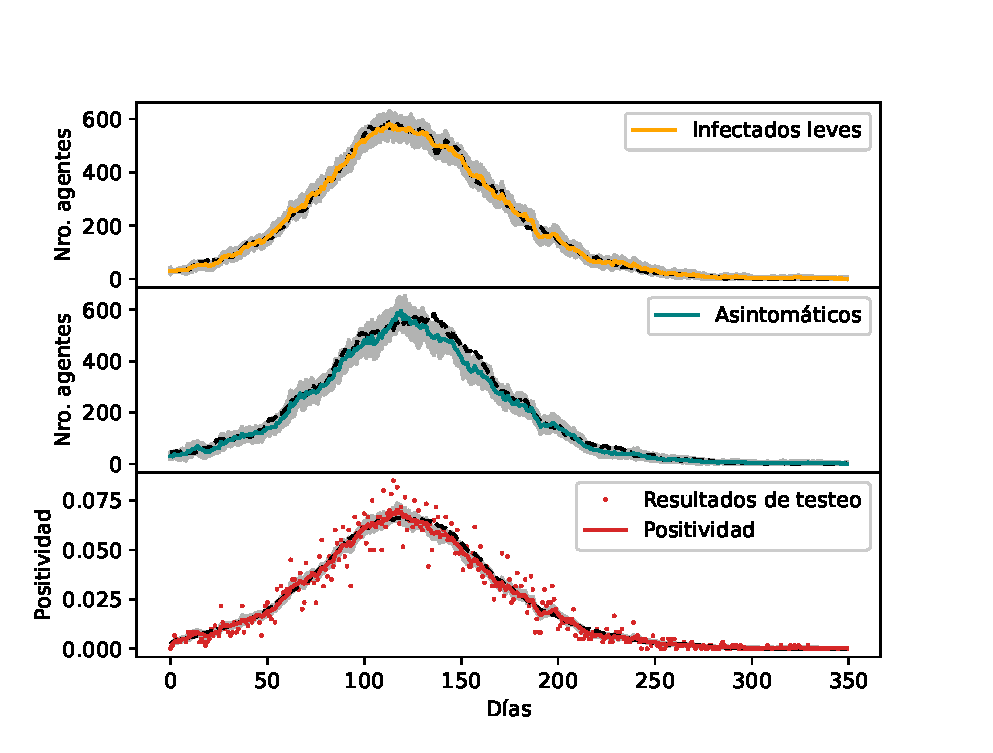
\includegraphics[width=0.75\textwidth]{abm_tests.eps}
    \caption{}
    \label{fig:abm_tests}
\end{figure}
\begin{figure}[h!]
    \centering
    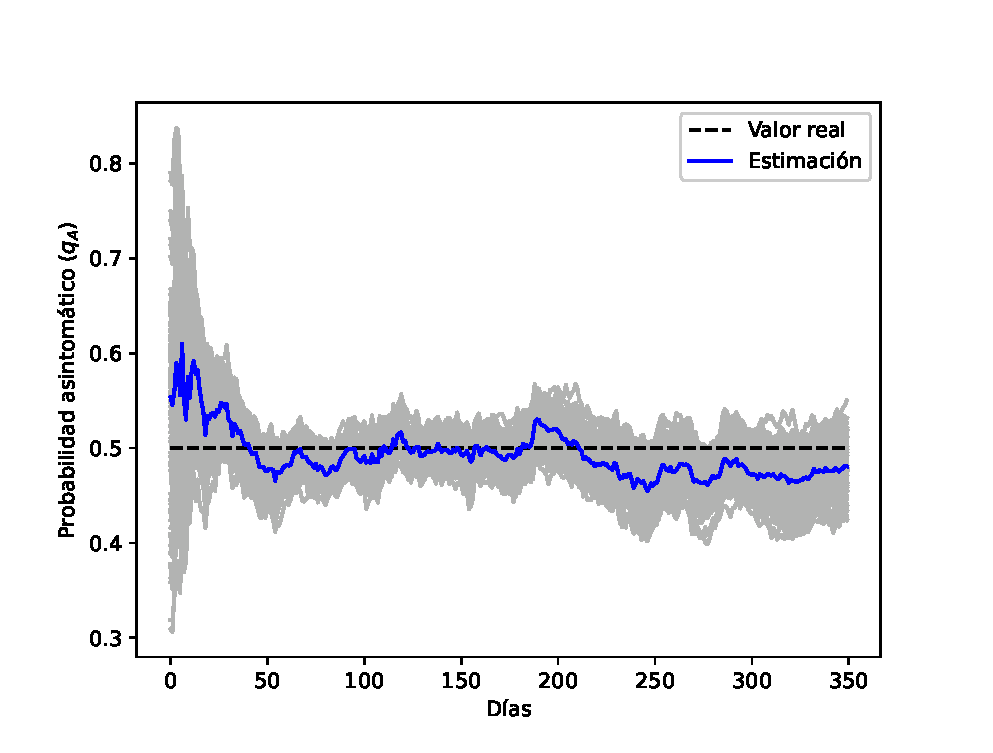
\includegraphics[width=0.75\textwidth]{abm_tests_asymptomatic_prob.eps}
    \caption{}
    \label{fig:abm_tests_asymptomatic_prob}
\end{figure}

\subsection{Datos CABA, Argentina}


\chapter{Conclusiones}

%----------------------------------------------------------------------------------------
%	THESIS CONTENT - APPENDICES
%----------------------------------------------------------------------------------------

\appendix % Cue to tell LaTeX that the following "chapters" are Appendices
\chapter{Asimilación de datos}
\section{Algoritmo \textit{forward-backward}}\label{appendix:ffbs}

El algoritmo \textit{forward-backward} está especificado en \ref{algo:ffbs}. 

\begin{algorithm}[H]\label{algo:ffbs}
    % \SetAlgoLined
    \SetKwInOut{Input}{input}\SetKwInOut{Output}{output}

    \Input{
        \par
        Distribución inicial $p(\v x_0)$
        \par
        Distribución de transición $p(\v x_t | \v x_{t-1})$ para $t = 1, ..., T$
        \par
        Verosimilitud observacional $p(\v y_t | \v x_t)$ para $t = 1, ..., T$ 
    }
    \Output{
        \par
        Distribución predictiva $p(\v x_t | \v y_{1:t-1})$ para para $t = 1, ..., T$
        \par
        Distribución filtrante $p(\v x_t | \v y_{1:t})$ para $t = 1, ..., T$
        \par
        Distribución suavizante $p(\v x_t | \v y_{1:T})$ para $t = 1, ..., T$ 
    }

    \hrulefill

    \textit{Forward filter}\

    \For{$t=1, ..., T$}{
        Computar distribución predictiva:\
        $p(\v x_t | \v y_{1:t-1}) = \int p(\v x_t | \v x_{t-1}) p(\v x_{t-1} | \v y_{1:t-1}) d\v x_{t-1}$\

        Computar distribución filtrante:\
        $p(\v x_t | \v y_{1:t}) \propto p(\v y_t | \v x_t) p(\v x_t | \v y_{1:t-1})$\
    }

    \textit{Backward smoother}\

    \For{$t=T, ..., 1$}{
        Computar distribución suavizante:\
        $p(\v x_t | \v y_{1:T}) = 
        \int \frac{p(\v x_{t+1} | \v x_t)p(\v x_t |\v y_{1:t})}
            {p(\v x_{t+1} |\v y_{1:t})}
            p(\v x_{t+1} | \v y_{1:T}) d\v x_{t+1}$\
    }
    \caption{Algoritmo forward filter backward smoothing}
\end{algorithm}


La distribución predictiva se puede deducir integrando la distribución de transición pesando con la distribución filtrante del paso anterior:
\begin{align}
    p(\v x_t | \v y_{1:t-1}) &= \int p(\v x_t, \v x_{t-1} | \v y_{1:t-1}) d\v x_{t-1} && \text{Marginalización}\\
    &= \int p(\v x_t | \v x_{t-1}, \v y_{1:t-1}) p(\v x_{t-1} | \v y_{1:t-1}) d\v x_{t-1} && \text{Bayes}\\
    &=\int p(\v x_t | \v x_{t-1}) p(\v x_{t-1} | \v y_{1:t-1}) d\v x_{t-1} && \text{Propiedades HMM}
\end{align}

Por otro lado, para obtener la distribución filtrante podemos usar la distribución predictiva e incorporar la información de la observación $\v y_t$ de la siguiente manera:
\begin{align}
    p(\v x_t | \v y_{1:t}) &= \frac
            {p(\v y_t | \v x_t \v y_{1:t-1}) p(\v x_t | \v y_{1:t-1})}
            {p(\v y_t | \v y_{1:t-1})} && \text{Bayes}\\
    &= \frac{p(\v y_t | \v x_t) p(\v x_t | \v y_{1:t-1})}
            {p(\v y_t | \v y_{1:t-1})} && \text{Propiedades HMM} \label{eq:forward_backward_filter_complete}\\
    &\propto p(\v y_t | \v x_t) p(\v x_t | \v y_{1:t-1})
\end{align}

Para calcular la distribución suavizante necesitamos tener las distribuciones filtrantes y predictivas del forward-pass e iterar desde la última observación hasta la primera:
\begin{align}
    p(\v x_t | \v y_{1:T}) &= 
        \int p(\v x_t | \v x_{t+1}, \v y_{1:T})
             p(\v x_{t+1} | \v y_{1:T}) d\v x_{t+1}
        && \text{Marginalización} \\
    &= \int p(\v x_t | \v x_{t+1}, \v y_{1:t})
             p(\v x_{t+1} | \v y_{1:T}) d\v x_{t+1}
        && \text{Propiedades HMM} \\
    &= \int \frac{p(\v x_{t+1} | \v x_t, \v y_{1:t})p(\v x_t |\v y_{1:t})}
            {p(\v x_{t+1} |\v y_{1:t})}
            p(\v x_{t+1} | \v y_{1:T}) d\v x_{t+1}
        && \text{Bayes} \\
    &= \int \frac{p(\v x_{t+1} | \v x_t)p(\v x_t |\v y_{1:t})}
            {p(\v x_{t+1} |\v y_{1:t})}
            p(\v x_{t+1} | \v y_{1:T}) d\v x_{t+1}
        && \text{Propiedades HMM}
\end{align}

\section{Filtro de Kalman}\label{appendix:kf}

La fórmula \ref{eq:kf_mean_pred} para la media $\v x_t^f$ de la distribución predictiva puede ser deducida de la siguiente manera:

\begin{align*}
    \v x_t^f &= E[\v X_t | \v y_{1:t-1}] && \text{Definición de $\v x_t^f$} \\
    &= \int \v x_t p(\v x_t | y_{1:t-1}) d\v x_t && \text{Definición de $E$} \\
    &= \int \v x_t \int p(\v x_t | \v x_{t-1}) p(\v x_{t-1} | \v y_{1:t-1}) d\v x_{t-1} d\v x_t && \text{Ec. \ref{eq:forward_pred}} \\
    &= \int p(\v x_{t-1} | \v y_{1:t-1}) \int \v x_t p(\v x_t | \v x_{t-1}) d\v x_t d\v x_{t-1} && \text{Intercambio de $\int$}\\ 
    &= \int p(\v x_{t-1} | \v y_{1:t-1}) E[\v X_t | \v x_{t-1}] d\v x_{t-1} && \text{Definición de $E$}\\
    &= \int p(\v x_{t-1} | \v y_{1:t-1}) E[\v M_t \v x_{t-1} + \gv\eta_t] d\v x_{t-1} && \text{Modelo}\\
    &= \int p(\v x_{t-1} | \v y_{1:t-1}) \v M_t \v x_{t-1} d\v x_{t-1} && \text{$\v M_t$ lineal y $E[\gv\eta_t] = 0$}\\
    &= \v M_t \int p(\v x_{t-1} | \v y_{1:t-1}) \v x_{t-1} d\v x_{t-1} && \text{Modelo} \\
    &= \v M_t E[\v X_{t-1} | \v y_{1:t-1}] && \text{$\v M_t$ lineal}\\
    &= \v M_t \v x_{t-1}^a && \text{Definición de $\v x_t^a$} &&
\end{align*}

Por otro lado, la fórmula \ref{eq:kf_var_pred} para la matriz de covarianza $\v P_t^f$ de la distribución predictiva puede ser obtenida como se detalla a continuación:
\begin{align*}
    \v P_t^f &= Var[\v X_t | \v y_{1:t-1}] && \text{Definición de $\v P_t^f$}\\ 
    &= E[\v X_t \v X_t^T | \v y_{1:t-1}] - E[\v X_t | \v y_{1:t-1}] E[\v X_t | \v y_{1:t-1}]^T && \text{$Var[\v X] = E[\v X \v X^T] - E[\v X]E[\v X]^T$} \\
    &= E[\v X_t \v X_t^T | \v y_{1:t-1}] - \v M_t \v x_{t-1}^a \v x_{t-1}^{aT} \v M_t^T && \text{Ec. \ref{eq:kf_mean_pred}}
\end{align*}
Ahora desarrollamos el valor esperado del primer término:
\begin{align*}
    E[&\v X_t \v X_t^T | \v y_{1:t-1}] = \int \v x_t \v x_t^T p(\v x_t | \v y_{1:t-1}) d\v x_t && \\
     &= \int \v x_t \v x_t^T \int p(\v x_t | \v x_{t-1}) p(\v x_{t-1} | \v y_{1:t-1}) d\v x_{t-1} d\v x_t && \text{Ec. \ref{eq:forward_pred}}\\
    &= \int p(\v x_{t-1} | \v y_{1:t-1}) \int \v x_t \v x_t^T p(\v x_t | \v x_{t-1}) d\v x_t d\v x_{t-1} && \text{Intercambio de $\int$}\\
    &= \int p(\v x_{t-1} | \v y_{1:t-1}) E[\v X_t \v X_t^T | \v x_{t-1}] d\v x_{t-1} && \text{Definición de $E$}\\
    &= \int p(\v x_{t-1} | \v y_{1:t-1}) (Var[\v X_t | \v x_{t-1}] && \text{$E[\v X \v X^T] = Var[\v X]^T + E[\v X]E[\v X]^T$}\\
    &\hspace{2em} + E[\v X_t | \v x_{t-1}]E[\v X_t | \v x_{t-1}]^T) d\v x_{t-1} && \\
    &= \int p(\v x_{t-1} | \v y_{1:t-1}) Var[\v X_t | \v x_{t-1}] d \v x_{t-1} && \text{Linealidad de $\int$}\\
    &\hspace{2em} + \int p(\v x_{t-1} | \v y_{1:t-1}) E[\v X_t | \v x_{t-1}]E[\v X_t | \v x_{t-1}]^T) d\v x_{t-1} && \\
    &= \int p(\v x_{t-1} | \v y_{1:t-1}) \v Q_t d \v x_{t-1} && \text{Ec. \ref{eq:kf_forward}}\\
    &\hspace{2em} + \int p(\v x_{t-1} | \v y_{1:t-1}) \v M_t \v x_{t-1} \v x_{t-1}^T \v M_t^T d\v x_{t-1} \\
    &= \v Q_t + \v M_t \int p(\v x_{t-1} | \v y_{1:t-1}) \v x_{t-1} \v x_{t-1}^T d\v x_{t-1} \v M_t^T && \text{$\v M_t$ lineal}\\
    &= \v Q_t + \v M_t E[\v X_{t-1} \v X_{t-1}^T | \v y_{1:t-1}] \v M_t^T && \text{Definición de $E$}\\
    &= \v Q_t + \v M_t E[\v X_{t-1} | \v y_{1:t-1}]E[\v X_{t-1} | \v y_{1:t-1}]^T \v M_t^T && \text{$E[\v X \v X^T] = Var[\v X] + E[\v X]E[\v X]^T$} \\
    &\hspace{2em} + \v M_t Var[\v X_{t-1} | \v y_{1:t-1}] \v M_t^T \\
    &= \v Q_t + \v M_t \v x_{t-1}^a \v x_{t-1}^{aT} \v M_t^T + \v M_t \v P_{t-1}^a \v M_t^T && \text{Definición de $\v x_{t-1}^a$ y $\v P_{t-1}^a$}\\
\end{align*}
Por lo tanto al combinar las expresiones obtenemos el resultado:
\begin{align*}
    \v P_t^f &= \v Q_t + \v M_t \v P_{t-1}^a \v M_t^T
\end{align*}

Para obtener las fórmulas de la media y covarianza de la distribución filtrante debemos usar la ecuación de análisis del algoritmo \textit{forward-backwards}:
\begin{align*}
    p(\v x_t | \v y_{1:t}) &\propto p(\v y_t | \v x_t) p(\v x_t | \v y_{1:t-1}) && \text{Ec. \ref{eq:forward_filt}} \\
    &\propto \exp((\v y_t - \v H_t \v x_t)^T \v R_t^{-1} (\v y_t - \v H_t \v x_t) && \text{Densidades Gaussianas}\\ 
    &+ (\v x_t - \v x_t^f)^T \v (\v P_t^{f})^{-1} (\v x_t - \v x_t^f)) \\
    &\propto \exp(\v x_t^T (\v (\v P_t^f)^{-1} + \v H^T \v R_t^{-1} \v H_t) \v x_t && \text{Distribución}\\
    &- 2 \v x_t^T (\v H^T \v R_t^{-1} \v y_t + (\v P_t^{f})^{-1} \v x_t)) \\
    &= \exp(\v x_t^T \v A \v x_t - 2\v x_t^T \v v) && \text{Renombre}\\
    &= \exp((\v x_t - \v A^{-1}\v v)^T \v A (\v x_t - \v A^{-1}\v v) - \v v^T \v A \v v) && \text{Completar cuadrados}\\
    &\propto \exp((\v x_t - \v A^{-1}\v v)^T \v A (\v x_t - \v A^{-1}\v v))
\end{align*}
donde hemos utilizado la siguiente nomenclatura:
\begin{align*}
    \v A &= \v (\v P_t^f)^{-1} + \v H^T \v R_t^{-1} \v H_t \\
    \v v &= \v H^T \v R_t^{-1} \v y_t + (\v P_t^{f})^{-1} \v x_t
\end{align*}.

La expresión que obtuvimos implica que la distribución filtrante es Gaussiana con media $\v A^{-1}\v v$ y covarianza $\v A^{-1}$. Vamos a desarrollar estas expresiones para obtener la formulación clásica del filtro de Kalman. Para ello, necesitaremos usar la siguiente identidad matricial de Woodbury \citep{Golub1996}:
\begin{align*}
    (\v A + \v C \v B \v C^T)^{-1} = \v A^{-1} - \v A^{-1} \v C (\v B^{-1} + \v C^T \v A^{-1} \v C)^{-1} \v C^T \v A^{-1}
\end{align*}

Tenemos entonces que:
\begin{align*}
    \v P_t^a &= \v A^{-1} && \\
    &= ((\v P_t^f)^{-1} + \v H^T \v R_t^{-1} \v H_t)^{-1} && \\
    &= \v P_t^f - \v P_t^f \v H_t^T (\v R_t + \v H \v P_t^f \v H^T)^{-1} \v H_t \v P_t^f && \text{Identidad de Woodbury}\\
    &= \v P_t^f - \v K_t \v H_t \v P_t^f && \\
    &= (\v I - \v K_t \v H_t) \v P_t^f && \\
\end{align*}
donde hemos definido a $\v K_t = \v P_t^f \v H_t^T (\v R_t + \v H \v P_t^f \v H^T)^{-1}$. Esta matriz es denominada matriz de ganancia de Kalman. Para desarrollar la expresión de la media de la distribución además usaremos la notación $\v S_t = (\v R_t + \v H \v P_t^f \v H^T)^{-1}$, con la cual la ganancia de Kalman se puede expresar como $\v K_t = \v P_t^f \v H_t^T \v S_t$ y podemos obtener la fórmula para $\v x_t^a$ de la siguiente manera:
\begin{align*}
    \v x_t^a &= \v A^{-1} \v v && \\
    &= (\v I - \v K_t \v H_t) (\v P_t^f \v H^T \v R_t^{-1} \v y_t + (\v P_t^{f})^{-1} \v x_t) && \\
    &= \v x_t - \v K_t \v H_t \v x_t + \v P_t \v H_t^T \v R_t^{-1} \v y_t - \v K_t \v H_t \v P_t \v H_t^T \v R_t^{-1} \v y_t && \\
    &= \v x_t - \v K_t \v H_t \v x_t + \v P_t \v H_t^T \v R_t^{-1} \v y_t - \v K_t \v H_t \v P_t \v H_t^T \v R_t^{-1} \v y_t && \\
    &= \v x_t - \v K_t \v H_t \v x_t + \v P_t \v H_t^T \v S_t \v S_t^{-1} \v R_t^{-1} \v y_t - \v K_t \v H_t \v P_t \v H_t^T \v R_t^{-1} \v y_t && \\
    &= \v x_t - \v K_t \v H_t \v x_t + \v K_t (\v R_t + \v H \v P_t^f \v H^T)^{-1} \v R_t^{-1} \v y_t - \v K_t \v H_t \v P_t \v H_t^T \v R_t^{-1} \v y_t && \\
    &= \v x_t - \v K_t \v H_t \v x_t + \v K_t \v y_t && \\
    &= \v x_t + \v K_t (\v y_t - \v H_t \v x_t) && \\
\end{align*}

\section{Filtro de partículas}\label{appendix:pf}

Hacemos aquí una deducción de el filtro de partículas SIR. El objetivo es obtener representaciones de partículas $\{\v x_t^{(i)}, w_t^{(i)}\}_{i=1}^{N}$ tal que sea una aproximación empírica de $p(\v x_t | \v y_{1:t})$. Vamos a comenzar por considerar la distribución conjunta de las variables de estado condicionadas a las observaciones, $p(\v x_{0:t} | \v y_{1:t})$. Estamos considerando a las variables de estado desde el tiempo $0$ hasta el $t$, lo cual significa que esta es la densidad de probabilidad de una trayectoria de las variables de estado en el tiempo. Claramente, si tenemos una muestra de esta distribución, las componentes correspondientes al tiempo $t$ constituirán una muestra de la probabilidad filtrante marginalizada $p(\v x_t | \v y_{1:t})$. Utilizando las propiedades Markovianas y la independencia condicional de las observaciones del modelo de Markov escondido podemos escribir:
\begin{align*}
    p(\v x_{0:t} | \v y_{1:t}) \propto p(\v x_{0:t-1} | \v y_{1:t}) p(\v x_t | \v x_{t-1}) p(\v y_t | \v x_t)
\end{align*}

Si muestreamos trayectorias $\{\v x_{0:t}^{(i)}\}_{i=1}^N$ de una probabilidad propuesta $q$ vamos a obtener que los pesos de importancia son 
\begin{align}\label{eq:importance_weights_general}
    w_t^{(i)} \propto \frac{p(\v x_{0:t-1} | \v y_{1:t}) p(\v x_t | \v x_{t-1}) p(\v y_t | \v x_t)}{q(\v x_{0:t})}
\end{align}

Adicionalmente consideraremos que $q$ cumple 
\begin{align}\label{eq:proposal_factor}
    q(\v x_{0:t} | \v y_{1:t}) = q(\v x_t | \v x_{0:t-1}, \v y_{1:t}) q(\v x_{0:t-1} | \v y_{1:t-1})
\end{align}
Esta factorización implica que si tenemos una muestra de la trayectoria $\v x_{0:t-1}^{(i)} \sim q(\v x_{0:t-1} | \v y_{1:t-1})$ entonces se puede obtener una muestra de la trayectoria hasta el tiempo $t$ incorporando la última componente muestreada como $\v x_t^{(i)} \sim q(\v x_t | \v x_{0:t-1}, \v y_{1:t})$.

Si entonces introducimos \ref{eq:proposal_factor} en \ref{eq:importance_weights_general}, tenemos que los pesos de importancia pueden ser computados como:
\begin{align*}
    w_t^{(i)} &\propto \frac{p(\v x_{0:t-1} | \v y_{1:t}) p(\v x_t | \v x_{t-1}) p(\v y_t | \v x_t)}{q(\v x_{0:t-1} | \v y_{1:t-1}) q(\v x_t | \v x_{0:t-1},  \v y_{1:t})} \\
    &\propto w_{t-1}^{(i)} \frac{p(\v x_t | \v x_{t-1}) p(\v y_t | \v x_t)}{q(\v x_t | \v x_{0:t-1},  \v y_{1:t})}
\end{align*}

Si adicionalmente dotamos a $q$ de ``Markovianidad'' en el sentido que $q(\v x_t | \v x_{0:t-1} \v y_{1:t}) = q(\v x_t | \v x_{t-1} \v y_t)$, entonces los pesos solamente dependen de $\v x_t$ y no de toda la trayectoria $\v x_{0:t-1}$. De esta manera se puede hacer filtrado de manera secuencial. Con estas suposiciones obtenemos la forma general de los pesos de el filtro de partículas SIR:
\begin{align*}
    w_t^{(i)} &\propto w_{t-1}^{(i)} \frac{p(\v x_t | \v x_{t-1}) p(\v y_t | \v x_t)}{q(\v x_t | \v x_{t-1}, \v y_t)}
\end{align*}

\section{EnKF} \label{appendix:enkf}

Para mostrar que la formulación del EnKF estocástico es correcta, basta probar que la media y covarianza que se obtiene de considerar a los miembros del ensamble como variables aleatorias coinciden con las del filtro de Kalman tradicional, el cual da una solución exacta al problema. Supongamos inductivamente que las partículas a tiempo $t-1$ cumplen con esto y veamos que podemos obtener las fórmulas correctas a tiempo $t$.

Las partículas del pronóstico están definidas como 
$$ \v x_t^{f, (i)} = \v M_t \v x_{t-1}^{a, (i)} + \gv\eta_t^{(i)}$$
con $\gv\eta_t^{(i)} \sim \mathcal{N}(\v 0, \v Q_t)$. Por lo tanto si calculamos la media y covarianza, obtenemos las mismas fórmulas que para el filtro de Kalman tradicional \ref{eq:kf_mean_pred} y \ref{eq:kf_var_pred}:
\begin{align*}
    E[\v x_t^{f, (i)}] &= E[\v M_t \v x_{t-1}^{a, (i)} + \gv\eta_t^{(i)}] \\
    &= \v M_t E[\v x_{t-1}^{a, (i)}] + E[\gv\eta_t^{(i)}] \\
    &= \v M_t \v x_{t-1}^a \\
    Var[\v x_t^{f, (i)}] &= Var[\v M_t \v x_{t-1}^{a, (i)} + \gv\eta_t^{(i)}] \\
    &= \v M_t Var[\v x_{t-1}^{a, (i)}] \v M_t^T + Var[\gv\eta_t^{(i)}] \\
    &= \v M_t \v P_t^a \v M_t^T + \v Q_t 
\end{align*}
donde hemos usado la independencia de $\gv\eta_t^{(i)}$ y $\v x_{t-1}^{a, (i)}$ y que $Var[\v A \v X] = \v A Var[\v X] \v A^T$ cuando $\v A$ es un operador lineal. Las partículas del pronóstico entonces constituyen efectivamente una muestra de la distribución del pronóstico.

Las partículas del análisis en el EnKF estocástico están definidas por 
$$ \v x_t^{a, (i)} = \v x_t^{f, (i)} + \widehat{\v K_t} (\v y_t - (\v H_t \v x_t^{f, (i)} + \v v_t^{(i)}))$$
donde $\v v_t^{(i)} \sim \mathcal{N}(\v 0, \v R_t)$ y la aproximación a la ganancia de Kalman es $\widehat{\v K}_t = \widehat{\v P}_t^f \v H_t^T(\v R_t + \v H_t \widehat{\v P}_t^f \v H_t^T)^{-1}$ con $\widehat{\v P}_t^f$ denotando la covarianza muestral del ensamble de pronóstico. Probaremos que en el caso ideal en que estemos usando la matriz de ganancia verdadera (es decir la que utiliza la covarianza exacta del pronóstico, $\v P_t^f$) la media y covarianza del ensamble del análisis coinciden con las del filtro de Kalman \ref{eq:kf_mean_filter} y \ref{eq:kf_var_filter}.
\begin{align*}
    E[\v x_t^{a, (i)}] &= E[\v x_t^{f, (i)} + \v K_t (\v y_t - (\v H_t \v x_t^{f, (i)} + \v v_t^{(i)}))] \\
    &= \v x_t^f + \v K_t E[(\v y_t - (\v H_t \v x_t^{f, (i)} + \v v_t^{(i)}))] \\
    &= \v x_t^f + \v K_t (\v y_t - E[\v H_t \v x_t^{f, (i)}]) \\
    &= \v x_t^f + \v K_t (\v y_t - \v H_t \v x_t^f)
\end{align*}
Por otro lado, para la varianza del ensamble de análisis tenemos que:
\begin{align*}
    Var[\v x_t^{a, (i)}] &= Var[\v x_t^{f, (i)} + \v K_t (\v y_t - (\v H_t \v x_t^{f, (i)} + \v v_t^{(i)}))] \\
    &= Var[\v x_t^{f, (i)}] + Var[\v K_t (\v y_t - (\v H_t \v x_t^{f, (i)} + \v v_t^{(i)}))] \\
    &+ 2 Cov[\v x_t^{f, (i)}, \v K_t (\v y_t - (\v H_t \v x_t^{f, (i)} + \v v_t^{(i)}))] \\
    &= \v P_t^f + \v K_t Var[(\v H_t \v x_t^{f, (i)} + \v v_t^{(i)})]\v K_t^T + 2 Cov[\v x_t^{f, (i)}, - \v K_t \v H_t \v x_t^{f, (i)}] \\ 
    &= \v P_t^f + \v K_t (\v H_t \v P_t^f \v H_t^T + \v R_t)\v K_t^T - 2 \v K_t \v H_t \v P_t^f \\
    &= \v P_t^f + \v P_t^f \v H_t^T (\v H_t \v P_t^f \v H_t^T + \v R_t)^{-1}(\v H_t \v P_t^f \v H_t^T + \v R_t)\v K_t^T - 2 \v K_t \v H_t \v P_t^f \\
    &= \v P_t^f + \v P_t^f \v H_t^T \v K_t^T - 2 \v K_t \v H_t \v P_t^f \\
    &= \v P_t^f + (\v K_t \v H_t \v P_t^f)^T - 2 \v K_t \v H_t \v P_t^f \\
    &= \v P_t^f - \v K_t \v H_t \v P_t^f \\
    &= (\v I - \v K_t \v H_t) \v P_t^f 
\end{align*}
donde hemos usado la propiedad de la varianza de una suma ($Var[\v X + \v Y] = Var[\v X] + Var[\v Y] + Cov[\v X, \v Y]$), la independencia de $\v x_t^{f, (i)}$ con $\v v_t^{(i)}$ y el hecho que $\v K_t \v H_t \v P_t^f$ es una matriz simétrica.

\chapter{Algoritmo EM}
\section{Gaussiana multivariada como miembro de la familia exponencial}\label{appendix:exp_family}

Aquí presentamos la representación de densidades de probabilidad de la familia exponencial y cómo se puede escribir a la Gaussiana como miembro de dicha familia. Luego damos la solución de la ecuación \ref{eq:null_elbo_grad} para encontrar el valor del parámetro que anula a la ELBO en el caso Gaussiano.

Se dice que una probabilidad pertenece a la familia exponencial si su densidad de probabilidad, parametrizada por $\gv\theta$ puede ser escrita como:
$$p(\v x; \gv\theta) = h(\v x) \exp(\psi(\gv\theta) \cdot S(\v x) - A(\gv\theta))$$
donde $S(\v x)$ es llamado el estadístico suficiente, $\psi(\gv \theta)$ la parametrización natural y $h$ y $A$ son funciones bien definidas \citep{Wasserman2004}. Es importante en esta representación, que la interacción entre $\v x$ y $\gv\theta$ se produce solamente a través del producto interno $\psi(\gv\theta)\cdot S(\v x)$. 

La densidad de probabilidad de una Gaussiana multivariada de dimensionalidad $N$ con media $\gv\mu$ y covarianza $\gv\Sigma$ es habitualmente expresada como:
$$p(\v x; \gv\theta) = (2\pi)^{-\frac{k}{2}} |\gv\Sigma|^{-\frac{1}{2}} \exp \{ - \frac{1}{2}(\v x- \gv\mu)^T \gv\Sigma^{-1}(\v x-\gv\mu) \}$$

Nuestro objetivo es expresar esta función con la forma de la familia exponencial considerando como parámetro solamente a la varianza $\gv\Sigma$ y considerando que $\gv\mu$ es conocido. Para ello consideremos la extensión del producto punto entre vectores a matrices como el producto Frobenious (elemento a elemento). Esto permite que la forma cuadrática dentro de la exponencial de la densidad Gaussiana se pueda reescribir como:
$$(\v x- \gv\mu)^T \gv\Sigma^{-1}(\v x-\gv\mu) = \gv\Sigma^{-1} \cdot ((\v x- \gv\mu) (\v x-\gv\mu)^T)$$
y por lo tanto logramos la forma de la familia exponencial usando:
\begin{align*}
    h(\v x) &= (2\pi)^{-\frac{N}{2}} \\
    \psi(\gv\theta) &=  -\frac{1}{2}\gv\Sigma^{-1} \\ 
    S(\v x) &= (\v x- \gv\mu) (\v x-\gv\mu)^T \\
    A(\gv\theta) &= \frac{1}{2} \log |\gv\Sigma|.
\end{align*} 

\section{Punto crítico de la ELBO en caso Gaussiano}\label{appendix:null_grad_elbo}

Aquí damos una solución para la ecuación \ref{eq:null_elbo_grad} en el caso Gaussiano utilizando la expresión de la densidad de probabilidad como miembro de la familia exponencial desarrollada en \ref{appendix:exp_family}:
\begin{align*}
    \nabla_{\gv\theta} \psi(\gv\theta) \cdot S - \nabla_{\gv\theta} A(\gv \theta) &= 0 \\
    -\frac{1}{2} \nabla_{\gv\Sigma}  (\v x- \gv\mu)^T \gv\Sigma^{-1}(\v x-\gv\mu) - \nabla_{\gv\Sigma} \frac{1}{2} \log |\gv\Sigma| &= 0 \\
    \frac{1}{2} \gv\Sigma^{-1} (\v x- \gv\mu)(\v x-\gv\mu)^T \gv\Sigma^{-1} - \frac{1}{2} \gv\Sigma^{-1} &= 0 \\
    \gv\Sigma^{-1} S \gv\Sigma^{-1} - \gv\Sigma^{-1} &= 0 \\
    S &= \gv\Sigma 
\end{align*}
donde hemos usado la expresión $\frac{\partial \log|\v X|}{\partial \v X} = \v X^{-T}$ para la derivada del logaritmo del determinante y $\frac{\partial \v a^T \v X^{-1} \v b }{\partial \v X} = \v X^{-T} \v a \v b^T \v X^{-1}$ para la derivada de la forma cuadrática \cite{Petersen2012}.

\section{Factorización de $p(\v x_{t-1}, \v x_t| \v y_{1:t})$} \label{appendix:IS_factorization}

Desarrollamos aquí la factorización de la probabilidad conjunta utilizada en \ref{eq:IS_factorization}.

\begin{align}
    p(\v x_{t-1}, \v x_t| \v y_{1:t}) &= p(\v x_{t-1} | \v x_t, \v y_{1:t}) p(\v x_t| \v y_{1:t}) && \text{Bayes} \\
    &= p(\v x_{t-1} | \v x_t, \v y_{1:t-1}) p(\v x_t| \v y_{1:t}) && \text{Prop. HMM} \\
    &= \frac{p(\v x_t| \v x_{t-1}, \v y_{1:t-1})p(\v x_{t-1} | \v y_{1:t-1})}{p(\v x_t |\v y_{1:t-1})} p(\v x_t| \v y_{1:t}) && \text{Bayes} \\
    &= p(\v x_t| \v x_{t-1})p(\v x_{t-1} | \v y_{1:t-1})\frac{p(\v x_t| \v y_{1:t})}{p(\v x_t |\v y_{1:t-1})} && \text{Prop. HMM} \\
    &= p(\v x_t| \v x_{t-1})p(\v x_{t-1} | \v y_{1:t-1})\frac{p(\v y_t| \v x_t)}{p(\v y_t |\v y_{1:t-1})} && \text{Ecuación \ref{eq:forward_backward_filter_complete}}
\end{align}

\section{Aproximación de la verosimilitud}\label{appendix:likelihood_montecarlo}

Desarrollamos aquí la aproximación de Monte Carlo utilizada en \ref{eq:likelihood_montecarlo}.

\begin{align*}
    \log p(\v y_{1:T}) &= \log \prod_{t=1}^{T} p(\v y_t | \v y_{1:t-1}) \\
    &= \log \prod_{t=1}^{T} \int p(\v y_t | \v x_t) p(\v x_t | \v y_{1:t-1}) d\v x_t \\
    &= \sum_{t=1}^{T} \log \int p(\v y_t | \v x_t) p(\v x_t | \v y_{1:t-1}) d\v x_t \\
    &\approx \sum_{t=1}^{T} \log \frac{1}{N_p} \sum_{j=1}^{N_p} p(\v y_t | \v x_t^{f, (j)})
\end{align*}
donde las partículas $\{\v x_t^{f, (j)}\}_{j=1}^{N_p}$ están muestreadas de la distribución de pronóstico $p(\v x_t | \v y_{1:t-1})$. La identidad utilizada en la primera línea se puede encontrar en \cite{Carrassi2017}


%----------------------------------------------------------------------------------------
%	BIBLIOGRAPHY
%----------------------------------------------------------------------------------------

\printbibliography[heading=bibintoc]

%----------------------------------------------------------------------------------------

\end{document}